\documentclass[oneside]{book}
\usepackage{color}
\usepackage{fancyhdr}
\usepackage{geometry}
\usepackage{graphicx}
\usepackage{ifthen}
\usepackage{makeidx}
\usepackage{moreverb}
\usepackage{times}
\usepackage{verbatim}
\usepackage{hyperref}
\usepackage{boxedminipage}
\usepackage{longtable}
\usepackage{multirow}


\geometry{letterpaper,margin=1in}

\pagestyle{fancy}
\fancyhf{}
\lhead{\bf\nouppercase\rightmark}
\rhead{\bf Page\space\thepage}

\newenvironment{entry}%
  {\begin{list}{}{\renewcommand{\makelabel}[1]%
    {\parbox[b]{\labelwidth}{\makebox[0pt][l]{\textbf{##1}}\\}}%
    \setlength{\labelwidth}{1em}%
    \setlength{\labelsep}{1em}%
    \setlength{\leftmargin}{2em}%
    \setlength{\topsep}{\medskipamount}%
    \setlength{\itemsep}{\medskipamount}%
    \setlength{\parsep}{\medskipamount}%
    \setlength{\listparindent}{0pt}}}
  {\end{list}}
\newenvironment{indented}%
  {\begin{list}{}{\setlength{\leftmargin}{2em}}%
    \setlength{\itemsep}{\medskipamount}%
    \setlength{\parsep}{\medskipamount}%
    \setlength{\listparindent}{0pt}\item}
  {\end{list}}

\let\keepttfamily\ttfamily
\def\ttfamily{\color{blue}\keepttfamily}
\def\listinglabel#1{\llap
  {\scriptsize\color{black}\the#1}\hskip\listingoffset\relax}

\newcommand\idx[2][xxx]{%
  \ifthenelse{\equal{#1}{xxx}}{\index{#2@\texttt{#2}}}%
  {\index{#2@\texttt{#2}}\index{#1!#2@\texttt{#2}}}}

\newlength{\BCL} % base class length, for base trees.

\newcommand\lal{\textsc{lal}}  
\newcommand\lalapps{\textsc{lalapps}}  
\newcommand\ligotools{\textsc{ligotools}}  

\bibliographystyle{lalapps}

\makeindex

\begin{document}

\frontmatter

\title{LALApps --- LSC Algorithm Library Applications}
\author{Contact: Duncan Brown \texttt{duncan@gravity.phys.uwm.edu}}
\maketitle

\thispagestyle{empty}
\chapter*{Authors}
\verbatiminput{AUTHORS}

\tableofcontents

\mainmatter

\color{black}
%\chapter{How to get, build and use software for the LSC Data Grid} 
%%
% $Id$
%
\color{black}
\chapter{How to get, build and use software for the LSC Data Grid} 
%%%%%%%%%%%%%%%%%%%%%%%%%%%%%%%%%%%%%%%%%%%%%%%%%%%%%%%%%%%%%%%%%%%%%%%%%%%
\section{Getting and installing the software}
%%%%%%%%%%%%%%%%%%%%%%%%%%%%%%%%%%%%%%%%%%%%%%%%%%%%%%%%%%%%%%%%%%%%%%%%%%%

We describe the installation of \lal\ and \lalapps\ for use in
gravitational-wave data analysis.   These packages are under active
development at the present time and the latest functionality is
available only from CVS.   These instructions assume a standard
RedHat installation including development tools.   

\subsection{Installation of required development tools}

A useful installation of \lal\ and \lalapps\ requires \textsc{fftw},
the \textsc{frame} and \textsc{metaio} libraries.   Pre-compiled
versions of these libraries are available as RPM's from
\begin{verbatim}
    http://www.lsc-group.phys.uwm.edu/lal/rpms/
\end{verbatim}
The binary versions
\begin{verbatim}
   fftw-2.1.3-2lal.i386.rpm   28-Aug-2003 17:35   810k  
   frame-6.08-1lal.i386.rpm   28-Aug-2003 17:35   464k  
   metaio-4.13-1lal.i386.rpm  28-Aug-2003 17:35    24k  
\end{verbatim}
are compiled on RedHat7.3 architecture,  but may work on later
versions of RedHat.   Download the RPM's,  log in as root on your
computer,  then type
\begin{verbatim}
rpm -Uvh fftw-2.1.3-2lal.i386.rpm
rpm -Uvh frame-6.08-1lal.i386.rpm
rpm -Uvh metaio-4.13-1lal.i386.rpm
\end{verbatim}
Watch for error messages.   If everything installs correctly,  skip to
Sec.~\ref{s:lal},  otherwise continue through the following steps.  

The source RPM's are also available on the LAL web site,   download
\begin{verbatim}
   fftw-2.1.3-2lal.src.rpm   28-Aug-2003 17:35   810k  
   frame-6.08-1lal.src.rpm   28-Aug-2003 17:35   464k  
   metaio-4.13-1lal.src.rpm  28-Aug-2003 17:35    24k  
\end{verbatim}
to your computer.  As root,   type
\begin{verbatim}
rpm -Uvh fftw-2.1.3-2lal.src.rpm
rpm -Uvh frame-6.08-1lal.src.rpm
rpm -Uvh metaio-4.13-1lal.src.rpm
\end{verbatim}
Watch for errors.  If this fails,  there is a major problem:  e-mail
\verb+lal-discuss@gravity.phys.uwm.edu+.    If it succeeds,  then
\begin{verbatim}
cd /usr/src/redhat/SPECS
rpm -ba fftw.spec
rpm -ba frame.spec
rpm -ba metaio.spec
cd ../RPMS/i386
rpm -Uvh fftw-2.1.3-2lal.i386.rpm
rpm -Uvh frame-6.08-1lal.i386.rpm
rpm -Uvh metaio-4.13-1lal.i386.rpm
\end{verbatim}
Watch for errors at every step.  If you encounter a problem:   e-mail
\verb+lal-discuss@gravity.phys.uwm.edu+.   If it succeeds,  then you
can go ahead to the next stage.

\color{black}
%%%%%%%%%%%%%%%%%%%%%%%%%%%%%%%%%%%%%%%%%%%%%%%%%%%%%%%%%%%%%%%%%%%%%%%%%%%
\subsection{Configuring your environment}
%%%%%%%%%%%%%%%%%%%%%%%%%%%%%%%%%%%%%%%%%%%%%%%%%%%%%%%%%%%%%%%%%%%%%%%%%%%
\color{black}

While developing,  we recommend that you install the \lal\ and \lalapps
somewhere under your home directory.  If you follow the
instructions below,  the \lal\ and \lalapps\ libraries will be in
\verb+$LALPREFIX/lib+;  the documentation in \verb+$LALPREFIX/doc+; the header
files in \verb+$LALPREFIX/include+; the binaries in \verb+$LALPREFIX/bin+.
The environment \verb+LALPREFIX+ should be set to the absolute path where you
want to install these things.  For example,  user \texttt{patrick} might put
the source code in \verb+/home/patrick/src+ and set \verb+LALPREFIX+ to
\verb+/home/patrick+.

We assume you have installed \ligotools\ and configured your
environment as described in Peter Shawhan's documentation.   
To make the appropriate binaries accesible to you,  check that your path is
set correctly. It is also useful to add environment variables for the CVS
servers. If you have a lal CVS login, change
\verb+anonymous@gravity.phys.uwm.edu+ to
\verb+your_user_name@gravity.phys.uwm.edu+ in the environment variables below.
If you are using \texttt{bash}, add
the following lines to your \texttt{.bash\_profile} file
\begin{verbatim}
export LALPREFIX=${HOME}      # <---- Change this as appropriate
export PATH=${LALPREFIX}/bin:${PATH}
export LALCVS=":pserver:anonymous@gravity.phys.uwm.edu:/usr/local/cvs/lal"
\end{verbatim}
If you are using \texttt{csh} or a derivative,  add the following lines to
your \texttt{.cshrc} file
\begin{verbatim}
setenv LALPREFIX $HOME
setenv PATH $LALPREFIX/bin:$PATH
setenv LALCVS ":pserver:anonymous@gravity.phys.uwm.edu:/usr/local/cvs/lal"
\end{verbatim}
These enviromnent variables must be set before running anything,
so it is a good idea to log out and log back in again before
continuing.   \textbf{Note:} With libtool version 1.4.2, or greater, there is
no need to have the \verb+LD_LIBRARY_PATH+ environment variable set. Library
paths are hard coded into the libraries using the \texttt{-rpath}
compiler option. This is the correct way to do this,  using
\verb+LD_LIBRARY_PATH+ is incorrect.  

\color{black}
%%%%%%%%%%%%%%%%%%%%%%%%%%%%%%%%%%%%%%%%%%%%%%%%%%%%%%%%%%%%%%%%%%%%%%%%%%%
\subsection{LAL}
%%%%%%%%%%%%%%%%%%%%%%%%%%%%%%%%%%%%%%%%%%%%%%%%%%%%%%%%%%%%%%%%%%%%%%%%%%%
\color{black}

In the following commands, remember \verb+LALPREFIX+ is the
absolute directory path where you want to install the LAL library.  If
\verb+LALPREFIX+ does not exist,  you must create it:
\begin{verbatim}
mkdir $LALPREFIX
\end{verbatim}
Then create the directory into which you wish to put the source files for LAL
and LALApps:
\begin{verbatim}
mkdir $LALPREFIX/src
\end{verbatim}

The LAL software is maintained in a CVS repository -- CVS stands for
Concurrent Version-control System which is tool to allow multiple developers
to manipulate the same software,  meerging differences and identifying
conflicts between changes if they arise.  Obtain the LAL package from the CVS
repository as follows:  
\begin{verbatim}
cd $LALPREFIX/src
cvs -d $LALCVS login
\end{verbatim}
At this point,  you will be asked for a password.  The password for the
\verb+anonymous+ user is \verb+lal+. If you have a your own username, use the
password that you have been given.
The version of LAL that is checked-out is identified by the argument
to the \texttt{-r} option in the commands below.   The HEAD tag checks out the
current development version.  If you want to check out a released
version, replace the \verb+HEAD+ tag by \verb+release-X-Y+ where
\verb+X+ and \verb+Y+ are integers which identify the release version
number as \verb+X.Y+.
\begin{verbatim}
cvs -d $LALCVS checkout -rHEAD lal
\end{verbatim}
You have now obtained the latest development version of LAL.

To build and install the LAL software suite, 
\begin{verbatim}
cd $LALPREFIX/src/lal
./00boot
./configure --prefix=$LALPREFIX \
        --enable-frame
make
make check
make dvi
make install prefix=$LALPREFIX/stow_pkgs/lal-howto
cd $LALPREFIX/stow_pkgs
stow lal-howto
\end{verbatim}
This completes the installation and testing of LAL.  

\color{black}
%%%%%%%%%%%%%%%%%%%%%%%%%%%%%%%%%%%%%%%%%%%%%%%%%%%%%%%%%%%%%%%%%%%%%%%%%%%
\subsection{LALApps}
%%%%%%%%%%%%%%%%%%%%%%%%%%%%%%%%%%%%%%%%%%%%%%%%%%%%%%%%%%%%%%%%%%%%%%%%%%%
\color{black}

In the following commands, remember \verb+LALPREFIX+ is the absolute
directory path where you want to install the LALApps binaries.  We
assume that you have followed the build instructions for \lal\ and
that the directories \verb+LALPREFIX+ and \verb+$LALPREFIX/src+ exist.

Obtain the LALApps package from the CVS repository as follows:  
\begin{verbatim}
cd $LALPREFIX/src
cvs -d $LALCVS login
\end{verbatim}
At this point,  you will be asked for a password.  The password for the
\verb+anonymous+ user is \verb+lal+. If you have your own username, use the
password that you have been given.
The version of LALApps that is checked-out is identified by the argument
to the \texttt{-r} option in the commands below.   The HEAD tag checks out the
current development version.  If you want to check out a released
version, replace the \verb+HEAD+ tag by \verb+release-X-Y+ where
\verb+X+ and \verb+Y+ are integers which identify the release version
number as \verb+X.Y+.
\begin{verbatim}
cvs -d $LALCVS checkout -rHEAD lalapps
\end{verbatim}
You have now obtained the latest development version of LALApps.

To build and install the LALApps suite, 
\begin{verbatim}
cd $LALPREFIX/src/lalapps
./00boot
./configure --prefix=$LALPREFIX \
    --with-extra-cppflags="-I$LALPREFIX/include" \
    --with-extra-ldflags="-L$LALPREFIX/lib" \
    --enable-frame
make
make check
make dvi
make install prefix=$LALPREFIX/stow_pkgs/lalapps-howto
cd $LALPREFIX/stow_pkgs
stow lalapps-howto
\end{verbatim}
This completes the installation and testing of LALApps.  

\begin{enumerate}

\item It's now time to start looking at the example search codes in the
\verb+contrib+ directory.  Either \verb+power+ or \verb+inspiral+ should serve
as good examples to get started.   Good luck and happy coding.

\end{enumerate}

\pagebreak
\begin{thebibliography}{99}
\bibitem{lalspec} Bruce Allen \textit{et al}, \emph{Numerical Algorithms
Library Specification and Style Guide}, distributed as part of \verb+lal+ 
package and LIGO-T990030.
\end{thebibliography}





\chapter{LALApps utilities}

Several utilities (macros, global variables, and functions) are provided to
assist in writing programs in LALApps, and for maintaining a standard
look-and-feel.  This chapter describes these utilities and concludes with
the listing of an example program.

\newpage
\section{Header \texttt{lalapps.h}}
\label{header:lalapps}

\begin{indented}
Provides utilities for writing programs for LALApps.

Several macros, global variables, and function prototypes are given that will
assist in writing LALApps programs, and will aid in maintaining a standard
look-and-feel.

To use these utilities, include the header \verb$lalapps.h$ and make sure the
program links to the object \verb$lalapps.o$.
\end{indented}

\newpage
\subsection{Function \texttt{set\_debug\_level}}
\label{function:set-debug-level}
\idx[Function]{set\_debug\_level}
\index{Debug Level}
\idx[Variable]{lalDebugLevel}
\idx[Debug Level]{lalDebugLevel}
\idx[Debug Level]{NDEBUG}
\idx[Debug Level]{ERROR}
\idx[Debug Level]{WARNING}
\idx[Debug Level]{INFO}
\idx[Debug Level]{TRACE}
\idx[Debug Level]{MEMINFO}
\idx[Debug Level]{MEMDBG}
\idx[Debug Level]{MSGLVL1}
\idx[Debug Level]{MSGLVL2}
\idx[Debug Level]{MSGLVL3}
\idx[Debug Level]{ALLDBG}
\idx[Environment]{LAL\_DEBUG\_LEVEL}

\begin{entry}

\item[Name]

\verb$set_debug_level$ --- sets the LAL debug level

\item[Synopsis]

\begin{verbatim}
#include <lalapps.h>
extern int lalDebugLevel;
int set_debug_level( const char *s );
\end{verbatim}

\item[Description]

The function \verb$set_debug_level$ sets the LAL debug level to a value
determined by the string \verb$s$, which can be an absolute debug level
(a string representing an integer) or a string of LAL debug level flags.
Allowed flags are:
\begin{indented}
\begin{entry}
\item[NDEBUG]
  No debugging information is printed and memory debugging code is disabled.
\item[ERROR]
  Error messages are printed.
\item[WARNING]
  Warning messages are printed.
\item[INFO]
  Information messages are printed.
\item[TRACE]
  Function call tracing messages are printed.
\item[MEMINFO]
  Memory allocation information messages are printed.
\item[MEMDBG]
  Debugging of memory allocation routines is enabled bug no messages are
  printed.
\end{entry}
\end{indented}
The following pre-defined composite levels are available:
\begin{indented}
\begin{entry}
\item[MSGLVL1]
  Equivalent to \verb$ERROR$.
\item[MSGLVL2]
  Equivalent to \verb$ERROR | WARNING$.
\item[MSGLVL3]
  Equivalent to \verb$ERROR | WARNING | INFO$.
\item[ALLDBG]
  All debugging messages are printed.
\end{entry}
\end{indented}

If the argument to \verb$set_debug_level$ is \verb$NULL$, then the string
stored in the environment variable \verb$LAL_DEBUG_LEVEL$ is used.  If this
environment is not defined, or if no flags or values are specified in the
string, the debug level is set to 0, which is equivalent to \verb$NDEBUG$.
(This is also the default value for \verb$lalDebugLevel$ unless it is set to
some other value.)

For example, the statement
\begin{indented}
\verb$set_debug_level( "ERROR | INFO" );$
\end{indented}
will set the debug level so that error and information messages are printed
(but not warning messages).  Another example is the statement
\begin{indented}
\verb$set_debug_level( "2" );$
\end{indented}
which would set the debug level to 2 (warning messages are printed).

\item[Return Value]

The return value is the (integer) debug level that is assigned to
\verb$lalDebugLevel$.

\item[Environment]
\leavevmode
\begin{entry}
\item[\texttt{LAL\_DEBUG\_LEVEL}]
  Default LAL debug level string to use.
\end{entry}

\end{entry}

\newpage
\subsection{Function \texttt{clear\_status}}
\label{function:clear-status}
\idx[Function]{clear\_status}
\idx[Variable]{blank\_status}

\begin{entry}

\item[Name]
\verb$clear_status$ --- clears the LAL status structure after a failed LAL
function call

\item[Synopsis]
\begin{verbatim}
#include <lalapps.h>
extern const LALStatus blank_status;
int clear_status( LALStatus *status );
\end{verbatim}

\item[Description]
Clears the LAL status structure and iteratively frees attatched (sic) any
linked status structures.  This is to be used after a failed LAL function
call to restore the status structure to a useable form.  The structure
\verb$blank_status$ contains a blank status structure that can be used to
initialize a status structure in the program.

\item[Example]

The following program calls a routine \verb$LALFailUnlessNegative$ twice,
once with a positive argument (which causes the routine to fail) and once
with a negative argument (which causes the routine to pass).  The function
\verb$clear_status$ is used to clean up the status structure after the
failure and the constant structure \verb$blank_status$ is used to initialize
the status structure.

\begin{indented}
\begin{verbatim}
#include <lalapps.h>
#include <lal/LALStdlib.h>

extern const LALStatus blank_status;

void LALFailUnlessNegative( LALStatus *status, INT4 n )
{
  INITSTATUS( status, "LALFail", "$Id$" );
  ATTATCHSTATUSPTR( status );
  ASSERT( n, status, 1, "Non-negative n" );
  if ( n > 0 )
  {
    TRY( LALFailUnlessNegative( status->statusPtr, n - 1 ), status );
  }
  DETATCHSTATUSPTR( status );
  RETURN( status );
}

int main( void )
{
  LALStatus status = blank_status;
  LALFailUnlessNegative( &status, 5 );
  clear_status( &status );
  LALFailUnlessNegative( &status, -2 );
  return status.statusCode;
}
\end{verbatim}
\end{indented}

\end{entry}


\newpage
\subsection{Macro \texttt{RCSID}}
\label{macro:RCSID}
\idx[Macro]{RCSID}
\idx[Variable]{rcsid}

\begin{entry}

\item[Name]

\verb$RCSID$ --- set the RCS Id variable

\item[Synopsis]

\begin{verbatim}
#include <lalapps.h>
#ifndef RCSID
#define RCSID( id ) static volatile const char *rcsid = (id)
#endif
\end{verbatim}

\item[Description]

\verb$RCSID$ sets the static (i.e., internal-linkage) variable \verb$rcsid$
to the RCS Id string, \$\relax Id\$, which is given as the argument \verb$id$.
The string \$\relax Id\$ is expanded by RCS to contain the identification of
the source file along with its revision number.
For example:
\begin{indented}
\verb+RCSID("$+\verb+Id+\verb+$");+
\end{indented}

\end{entry}

\newpage
\subsection{Macro \texttt{PRINT\_VERSION}}
\label{macro:PRINT-VERSION}
\idx[Macro]{PRINT\_VERSION}

\begin{entry}

\item[Name]
\verb$PRINT_VERSION$ --- prints the LALApps version of the program

\item[Synopsis]
\begin{verbatim}
#include <lalapps.h>
static volatile const char *rcsid="$Id$";
#ifndef PRINT_VERSION
#define PRINT_VERSION( program ) \
  fprintf( stderr, PACKAGE " %s version " VERSION "\n%s\n", program, rcsid )
#endif
\end{verbatim}

\item[Description]
\verb$PRINT_VERSION$ prints the version information for \verb$program$ in a
standard format, along with the RCS Id information.  For example, for the
program \verb$lalapps_hello$, the version information
\begin{indented}
\verb+lalapps hello version 0.1+\\
\verb+$+\verb+Id+\verb+$+
\end{indented}
is printed with the command \verb$lalapps_hello -V$.  The source code to
print this is
\begin{indented}
\verb$PRINT_VERSION( "hello" );$
\end{indented}

Note that \verb$PRINT_VERSION$ requires the string variable \verb$rcsid$ to be
set.

\end{entry}

\newpage
\subsection{Macro \texttt{LAL\_CALL}}
\label{macro:LAL-CALL}
\idx[Macro]{LAL\_CALL}
\idx[Variable]{vrblvl}
\idx[Function]{lal\_errhandler}
\idx[Type]{lal\_errhandler\_t}
\index{Error Handler}
\idx[Error Handler]{LAL\_ERR\_DFLT}
\idx[Error Handler]{LAL\_ERR\_ABRT}
\idx[Error Handler]{LAL\_ERR\_EXIT}
\idx[Error Handler]{LAL\_ERR\_RTRN}

\begin{entry}

\item[Name]
\verb$LAL_CALL$ --- call a LAL routine and handle any errors

\item[Synopsis]
\begin{verbatim}
#include <lalapps.h>

extern int vrblvl;
extern int ( *lal_errhandler )( LALStatus *stat, const char *func,
    const char *file, const int line, volatile const char *id );
extern lal_errhandler_t lal_errhandler;

static volatile const char *rcsid="$Id$";

#ifndef LAL_CALL
#define LAL_CALL( function, statusptr ) \
  ((function),lal_errhandler(statusptr,#function,__FILE__,__LINE__,rcsid))
#endif
\end{verbatim}

\item[Description]
\verb$LAL_CALL$ executes the LAL function \verb$function$ and executes the
error handler \verb$lal_errhandler$, which examines the status structure
\verb$statusptr$ to see if an error occurred.  Typically the error handler
will return with value 0 if there was no error; otherwise it will print a trace
of the execution stack and then perform a specific action.  The action
performed depends on the error handler, which can be set to one of the
following:
\begin{indented}
\begin{entry}
\item[\texttt{LAL\_ERR\_DFLT}]
  The default error handler (same as \verb$LAL_ERR_ABRT$).
\item[\texttt{LAL\_ERR\_ABRT}]
  Raises \verb$SIGABRT$ if there is an error.
\item[\texttt{LAL\_ERR\_EXIT}]
  Exits with the returned status code if there is an error.
\item[\texttt{LAL\_ERR\_RTRN}]
  Returns the status code.
\end{entry}
\end{indented}

Note that \verb$LAL_CALL$ requires the string variable \verb$rcsid$ to be set.

\item[Return Value]
If \verb$LAL_CALL$ returns (rather than terminating execution), the return
value is equal to the status code returned by the LAL function.

\item[Example]
The following example program illustrates the use of \verb$LAL_CALL$.
The routine \verb$LALInvert$ is called incorrectly twice.  The first time
the division by zero error is caught.  The second time, the unexpected null
pointer error is not caught and the default error handler aborts the program.
\begin{indented}
\begin{verbatim}
#include <stdlib.h>
#include <lalapps.h>
#include <lal/LALStdlib.h>

RCSID( "$Id$" );

extern int vrblvl;
extern const LALStatus blank_status;

void LALInvert( LALStatus *status, REAL4 *y, REAL4 x )
{
  INITSTATUS( status, "LALInvert", rcsid );
  ASSERT( y, status, 1, "Null pointer" );
  if ( input == 0 )
  {
    ABORT( status, 1, "Division by zero" );
  }
  *y = 1 / x;
  RETURN( status );
}

int main( void )
{
  LALStatus status = blank_status;
  REAL4 x;
  int code;

  vrblvl = 1;

  lal_errhandler = LAL_ERR_RTRN;
  code = LAL_CALL( LALInvert( &status, &x, 0 ), &status );
  if ( code == 2 )
  {
    puts( "division by zero" );
    clear_status( &status );
  }
  else if ( code )
  {
    exit( code );
  }

  lal_errhandler = LAL_ERR_DFLT;
  LAL_CALL( LALInvert( &status, NULL, 1 ), &status );

  return 0;
}
\end{verbatim}
\end{indented}

\end{entry}

\newpage
\section{Source \texttt{hello.c}}
\label{source:hello.c}
\idx[Source]{hello.c}

\begin{indented}
This is the source code for the program \verb$lalapps_hello$:

\listinginput[10]{1}{hello.c}
\end{indented}

\newpage
%
% API Documentation
% Module pipeline
%
% Generated by epydoc 2.0
% [Thu Sep 25 14:02:49 2003]
%

%%%%%%%%%%%%%%%%%%%%%%%%%%%%%%%%%%%%%%%%%%%%%%%%%%%%%%%%%%%%%%%%%%%%%%%%%%%
%%                          Module Description                           %%
%%%%%%%%%%%%%%%%%%%%%%%%%%%%%%%%%%%%%%%%%%%%%%%%%%%%%%%%%%%%%%%%%%%%%%%%%%%

    \index{pipeline \textit{(module)}|(}
\section{Python Module \texttt{pipeline}}

    \label{pipeline}
This modules contains objects that make it simple for the user to create 
python scripts that build Condor DAGs to run code on the LSC Data Grid.


%%%%%%%%%%%%%%%%%%%%%%%%%%%%%%%%%%%%%%%%%%%%%%%%%%%%%%%%%%%%%%%%%%%%%%%%%%%
%%                               Functions                               %%
%%%%%%%%%%%%%%%%%%%%%%%%%%%%%%%%%%%%%%%%%%%%%%%%%%%%%%%%%%%%%%%%%%%%%%%%%%%

  \subsection{Functions}

    \label{pipeline:s2play}
    \index{pipeline \textit{(module)}!s2play \textit{(function)}}
    \vspace{0.5ex}

    \noindent\begin{boxedminipage}{\textwidth}

    \raggedright \textbf{s2play}(\textit{t})

    \vspace{-1.5ex}

    \rule{\textwidth}{0.5\fboxrule}
    Return 1 if t is in the S2 playground, 0 otherwise t = GPS time to 
    test if playground

    \vspace{1ex}

    \end{boxedminipage}


%%%%%%%%%%%%%%%%%%%%%%%%%%%%%%%%%%%%%%%%%%%%%%%%%%%%%%%%%%%%%%%%%%%%%%%%%%%
%%                               Variables                               %%
%%%%%%%%%%%%%%%%%%%%%%%%%%%%%%%%%%%%%%%%%%%%%%%%%%%%%%%%%%%%%%%%%%%%%%%%%%%

  \subsection{Variables}

\begin{longtable}{|p{.30\textwidth}|p{.62\textwidth}|l}
\cline{1-2}
\cline{1-2} \centering \textbf{Name} & \centering \textbf{Description}& \\
\cline{1-2}
\endhead\cline{1-2}\multicolumn{3}{r}{\small\textit{continued on next page}}\\\endfoot\cline{1-2}
\endlastfoot\raggedright \_\-\_\-a\-u\-t\-h\-o\-r\-\_\-\_\- & \raggedright \textbf{Value:} 
{\tt '\-D\-u\-n\-c\-a\-n\-~\-B\-r\-o\-w\-n\-~\-{\textless}\-d\-u\-n\-c\-a\-n\-@\-g\-r\-a\-v\-i\-t\-y\-.\-p\-h\-y\-s\-.\-u\-w\-m\-.\-e\-d\-u\-{\textgreater}\-'\-}&\\
\cline{1-2}
\raggedright \_\-\_\-d\-a\-t\-e\-\_\-\_\- & \raggedright \textbf{Value:} 
{\tt '\-\$\-D\-a\-t\-e\-:\-~\-2\-0\-0\-3\-/\-1\-0\-/\-0\-1\-~\-0\-8\-:\-4\-6\-:\-0\-6\-~\-\$\-'\-}&\\
\cline{1-2}
\raggedright \_\-\_\-v\-e\-r\-s\-i\-o\-n\-\_\-\_\- & \raggedright \textbf{Value:} 
{\tt '\-1\-.\-1\-8\-'\-}&\\
\cline{1-2}
\end{longtable}

    \index{pipeline \textit{(module)}!AnalysisChunk \textit{(class)}|(}

%%%%%%%%%%%%%%%%%%%%%%%%%%%%%%%%%%%%%%%%%%%%%%%%%%%%%%%%%%%%%%%%%%%%%%%%%%%
%%                           Class Description                           %%
%%%%%%%%%%%%%%%%%%%%%%%%%%%%%%%%%%%%%%%%%%%%%%%%%%%%%%%%%%%%%%%%%%%%%%%%%%%

\subsection{Class AnalysisChunk}

    \label{pipeline:AnalysisChunk}
An AnalysisCunk is the unit of data that a node works with, usually some 
subset of a ScienceSegment.


%%%%%%%%%%%%%%%%%%%%%%%%%%%%%%%%%%%%%%%%%%%%%%%%%%%%%%%%%%%%%%%%%%%%%%%%%%%
%%                                Methods                                %%
%%%%%%%%%%%%%%%%%%%%%%%%%%%%%%%%%%%%%%%%%%%%%%%%%%%%%%%%%%%%%%%%%%%%%%%%%%%

  \subsubsection{Methods}

    \label{pipeline:AnalysisChunk:__init__}
    \index{pipeline \textit{(module)}!AnalysisChunk \textit{(class)}!\_\_init\_\_ \textit{(method)}}
    \vspace{0.5ex}

    \noindent\begin{boxedminipage}{\textwidth}

    \raggedright \textbf{\_\_init\_\_}(\textit{self}, \textit{start}, \textit{end})

    \vspace{-1.5ex}

    \rule{\textwidth}{0.5\fboxrule}
    start = GPS start time of the chunk. end = GPS end time of the chunk.

    \vspace{1ex}

    \end{boxedminipage}

    \label{pipeline:AnalysisChunk:__len__}
    \index{pipeline \textit{(module)}!AnalysisChunk \textit{(class)}!\_\_len\_\_ \textit{(method)}}
    \vspace{0.5ex}

    \noindent\begin{boxedminipage}{\textwidth}

    \raggedright \textbf{\_\_len\_\_}(\textit{self})

    \vspace{-1.5ex}

    \rule{\textwidth}{0.5\fboxrule}
    Returns the length of this AnalysisChunk in seconds.

    \vspace{1ex}

    \end{boxedminipage}
    
    \label{pipeline:AnalysisChunk:__repr__}
    \index{pipeline \textit{(module)}!AnalysisChunk \textit{(class)}!\_\_repr\_\_ \textit{(method)}}
    \vspace{0.5ex}

    \noindent\begin{boxedminipage}{\textwidth}

    \raggedright \textbf{\_\_repr\_\_}(\textit{self})

    \end{boxedminipage}

    \label{pipeline:AnalysisChunk:dur}
    \index{pipeline \textit{(module)}!AnalysisChunk \textit{(class)}!dur \textit{(method)}}
    \vspace{0.5ex}

    \noindent\begin{boxedminipage}{\textwidth}

    \raggedright \textbf{dur}(\textit{self})

    \vspace{-1.5ex}

    \rule{\textwidth}{0.5\fboxrule}
    Returns the length (duration) of the chunk in seconds.

    \vspace{1ex}

    \end{boxedminipage}

    \label{pipeline:AnalysisChunk:end}
    \index{pipeline \textit{(module)}!AnalysisChunk \textit{(class)}!end \textit{(method)}}
    \vspace{0.5ex}

    \noindent\begin{boxedminipage}{\textwidth}

    \raggedright \textbf{end}(\textit{self})

    \vspace{-1.5ex}

    \rule{\textwidth}{0.5\fboxrule}
    Returns the GPS end time of the chunk.

    \vspace{1ex}

    \end{boxedminipage}

    \label{pipeline:AnalysisChunk:start}
    \index{pipeline \textit{(module)}!AnalysisChunk \textit{(class)}!start \textit{(method)}}
    \vspace{0.5ex}

    \noindent\begin{boxedminipage}{\textwidth}

    \raggedright \textbf{start}(\textit{self})

    \vspace{-1.5ex}

    \rule{\textwidth}{0.5\fboxrule}
    Returns the GPS start time of the chunk.

    \vspace{1ex}

    \end{boxedminipage}

    \index{pipeline \textit{(module)}!AnalysisChunk \textit{(class)}|)}
    \index{pipeline \textit{(module)}!AnalysisJob \textit{(class)}|(}

%%%%%%%%%%%%%%%%%%%%%%%%%%%%%%%%%%%%%%%%%%%%%%%%%%%%%%%%%%%%%%%%%%%%%%%%%%%
%%                           Class Description                           %%
%%%%%%%%%%%%%%%%%%%%%%%%%%%%%%%%%%%%%%%%%%%%%%%%%%%%%%%%%%%%%%%%%%%%%%%%%%%

\subsection{Class AnalysisJob}

    \label{pipeline:AnalysisJob}
Describes a generic analysis job that filters LIGO data as configured by 
an ini file.


%%%%%%%%%%%%%%%%%%%%%%%%%%%%%%%%%%%%%%%%%%%%%%%%%%%%%%%%%%%%%%%%%%%%%%%%%%%
%%                                Methods                                %%
%%%%%%%%%%%%%%%%%%%%%%%%%%%%%%%%%%%%%%%%%%%%%%%%%%%%%%%%%%%%%%%%%%%%%%%%%%%

  \subsubsection{Methods}

    \label{pipeline:AnalysisJob:__init__}
    \index{pipeline \textit{(module)}!AnalysisJob \textit{(class)}!\_\_init\_\_ \textit{(method)}}
    \vspace{0.5ex}

    \noindent\begin{boxedminipage}{\textwidth}

    \raggedright \textbf{\_\_init\_\_}(\textit{self}, \textit{cp})

    \vspace{-1.5ex}

    \rule{\textwidth}{0.5\fboxrule}
    cp = ConfigParser object that contains the configuration for this 
    job.

    \vspace{1ex}

    \end{boxedminipage}

    \label{pipeline:AnalysisJob:calibration}
    \index{pipeline \textit{(module)}!AnalysisJob \textit{(class)}!calibration \textit{(method)}}
    \vspace{0.5ex}

    \noindent\begin{boxedminipage}{\textwidth}

    \raggedright \textbf{calibration}(\textit{self}, \textit{ifo})

    \vspace{-1.5ex}

    \rule{\textwidth}{0.5\fboxrule}
    Returns the name of the calibration file to use for the given IFO. 
    ifo = name of interferomener (e.g. L1, H1 or H2).

    \vspace{1ex}

    \end{boxedminipage}

    \label{pipeline:AnalysisJob:channel}
    \index{pipeline \textit{(module)}!AnalysisJob \textit{(class)}!channel \textit{(method)}}
    \vspace{0.5ex}

    \noindent\begin{boxedminipage}{\textwidth}

    \raggedright \textbf{channel}(\textit{self})

    \vspace{-1.5ex}

    \rule{\textwidth}{0.5\fboxrule}
    Returns the name of the channel that this job is filtering. Note that 
    channel is defined to be IFO independent, so this may be LSC-AS\_Q or 
    IOO-MC\_F. The IFO is set on a per node basis, not a per job basis.

    \vspace{1ex}

    \end{boxedminipage}

    \label{pipeline:AnalysisJob:get_config}
    \index{pipeline \textit{(module)}!AnalysisJob \textit{(class)}!get\_config \textit{(method)}}
    \vspace{0.5ex}

    \noindent\begin{boxedminipage}{\textwidth}

    \raggedright \textbf{get\_config}(\textit{self}, \textit{sec}, \textit{opt})

    \vspace{-1.5ex}

    \rule{\textwidth}{0.5\fboxrule}
    Get the configration variable in a particular section of this jobs 
    ini file. sec = ini file section. opt = option from section sec.

    \vspace{1ex}

    \end{boxedminipage}

    \index{pipeline \textit{(module)}!AnalysisJob \textit{(class)}|)}
    \index{pipeline \textit{(module)}!AnalysisNode \textit{(class)}|(}

%%%%%%%%%%%%%%%%%%%%%%%%%%%%%%%%%%%%%%%%%%%%%%%%%%%%%%%%%%%%%%%%%%%%%%%%%%%
%%                           Class Description                           %%
%%%%%%%%%%%%%%%%%%%%%%%%%%%%%%%%%%%%%%%%%%%%%%%%%%%%%%%%%%%%%%%%%%%%%%%%%%%

\subsection{Class AnalysisNode}

    \label{pipeline:AnalysisNode}
\begin{tabular}{cccccc}
% Line for pipeline.CondorDAGNode, linespec=[0]
\multicolumn{2}{r}{\settowidth{\BCL}{pipeline.CondorDAGNode}\multirow{2}{\BCL}{pipeline.CondorDAGNode}}
&&
  \\\cline{3-3}
  &&\multicolumn{1}{c|}{}
&&
  \\
&&\multicolumn{2}{l}{\textbf{AnalysisNode}}
\end{tabular}

Contains the methods that allow an object to be built to analyse LIGO 
data in a Condor DAG.


%%%%%%%%%%%%%%%%%%%%%%%%%%%%%%%%%%%%%%%%%%%%%%%%%%%%%%%%%%%%%%%%%%%%%%%%%%%
%%                                Methods                                %%
%%%%%%%%%%%%%%%%%%%%%%%%%%%%%%%%%%%%%%%%%%%%%%%%%%%%%%%%%%%%%%%%%%%%%%%%%%%

  \subsubsection{Methods}

    \label{pipeline:AnalysisNode:__init__}
    \index{pipeline \textit{(module)}!AnalysisNode \textit{(class)}!\_\_init\_\_ \textit{(method)}}
    \vspace{0.5ex}

    \noindent\begin{boxedminipage}{\textwidth}

    \raggedright \textbf{\_\_init\_\_}(\textit{self})

      Overrides: pipeline.CondorDAGNode.\_\_init\_\_

    \end{boxedminipage}

    \label{pipeline:AnalysisNode:get_end}
    \index{pipeline \textit{(module)}!AnalysisNode \textit{(class)}!get\_end \textit{(method)}}
    \vspace{0.5ex}

    \noindent\begin{boxedminipage}{\textwidth}

    \raggedright \textbf{get\_end}(\textit{self})

    \vspace{-1.5ex}

    \rule{\textwidth}{0.5\fboxrule}
    Get the GPS end time of the node.

    \vspace{1ex}

    \end{boxedminipage}

    \label{pipeline:AnalysisNode:get_ifo}
    \index{pipeline \textit{(module)}!AnalysisNode \textit{(class)}!get\_ifo \textit{(method)}}
    \vspace{0.5ex}

    \noindent\begin{boxedminipage}{\textwidth}

    \raggedright \textbf{get\_ifo}(\textit{self})

    \vspace{-1.5ex}

    \rule{\textwidth}{0.5\fboxrule}
    Returns the two letter IFO code for this node.

    \vspace{1ex}

    \end{boxedminipage}

    \label{pipeline:AnalysisNode:get_input}
    \index{pipeline \textit{(module)}!AnalysisNode \textit{(class)}!get\_input \textit{(method)}}
    \vspace{0.5ex}

    \noindent\begin{boxedminipage}{\textwidth}

    \raggedright \textbf{get\_input}(\textit{self})

    \vspace{-1.5ex}

    \rule{\textwidth}{0.5\fboxrule}
    Get the file that will be passed as input.

    \vspace{1ex}

    \end{boxedminipage}

    \label{pipeline:AnalysisNode:get_output}
    \index{pipeline \textit{(module)}!AnalysisNode \textit{(class)}!get\_output \textit{(method)}}
    \vspace{0.5ex}

    \noindent\begin{boxedminipage}{\textwidth}

    \raggedright \textbf{get\_output}(\textit{self})

    \vspace{-1.5ex}

    \rule{\textwidth}{0.5\fboxrule}
    Get the file that will be passed as output.

    \vspace{1ex}

    \end{boxedminipage}

    \label{pipeline:AnalysisNode:get_start}
    \index{pipeline \textit{(module)}!AnalysisNode \textit{(class)}!get\_start \textit{(method)}}
    \vspace{0.5ex}

    \noindent\begin{boxedminipage}{\textwidth}

    \raggedright \textbf{get\_start}(\textit{self})

    \vspace{-1.5ex}

    \rule{\textwidth}{0.5\fboxrule}
    Get the GPS start time of the node.

    \vspace{1ex}

    \end{boxedminipage}

    \label{pipeline:AnalysisNode:set_cache}
    \index{pipeline \textit{(module)}!AnalysisNode \textit{(class)}!set\_cache \textit{(method)}}
    \vspace{0.5ex}

    \noindent\begin{boxedminipage}{\textwidth}

    \raggedright \textbf{set\_cache}(\textit{self}, \textit{file})

    \vspace{-1.5ex}

    \rule{\textwidth}{0.5\fboxrule}
    Set the LAL frame cache to to use. The frame cache is passed to the 
    job with the --frame-cache argument. file = calibration file to use.

    \vspace{1ex}

    \end{boxedminipage}

    \label{pipeline:AnalysisNode:set_end}
    \index{pipeline \textit{(module)}!AnalysisNode \textit{(class)}!set\_end \textit{(method)}}
    \vspace{0.5ex}

    \noindent\begin{boxedminipage}{\textwidth}

    \raggedright \textbf{set\_end}(\textit{self}, \textit{time})

    \vspace{-1.5ex}

    \rule{\textwidth}{0.5\fboxrule}
    Set the GPS end time of the analysis node by setting a --gps-end-time 
    option to the node when it is executed. time = GPS end time of job.

    \vspace{1ex}

    \end{boxedminipage}

    \label{pipeline:AnalysisNode:set_ifo}
    \index{pipeline \textit{(module)}!AnalysisNode \textit{(class)}!set\_ifo \textit{(method)}}
    \vspace{0.5ex}

    \noindent\begin{boxedminipage}{\textwidth}

    \raggedright \textbf{set\_ifo}(\textit{self}, \textit{ifo})

    \vspace{-1.5ex}

    \rule{\textwidth}{0.5\fboxrule}
    Set the channel name to analyze and add a calibration file for that 
    channel. The name of the ifo is prepended to the channel name 
    obtained from the job configuration file and passed with a 
    --channel-name option. A calibration file is obtained from the ini 
    file and passed with a --calibration-cache option. ifo = two letter 
    ifo code (e.g. L1, H1 or H2).

    \vspace{1ex}

    \end{boxedminipage}

    \label{pipeline:AnalysisNode:set_input}
    \index{pipeline \textit{(module)}!AnalysisNode \textit{(class)}!set\_input \textit{(method)}}
    \vspace{0.5ex}

    \noindent\begin{boxedminipage}{\textwidth}

    \raggedright \textbf{set\_input}(\textit{self}, \textit{file})

    \vspace{-1.5ex}

    \rule{\textwidth}{0.5\fboxrule}
    Add an input to the node by adding a --input option. file = option 
    argument to pass as input.

    \vspace{1ex}

    \end{boxedminipage}

    \label{pipeline:AnalysisNode:set_output}
    \index{pipeline \textit{(module)}!AnalysisNode \textit{(class)}!set\_output \textit{(method)}}
    \vspace{0.5ex}

    \noindent\begin{boxedminipage}{\textwidth}

    \raggedright \textbf{set\_output}(\textit{self}, \textit{file})

    \vspace{-1.5ex}

    \rule{\textwidth}{0.5\fboxrule}
    Add an output to the node by adding a --output option. file = option 
    argument to pass as output.

    \vspace{1ex}

    \end{boxedminipage}

    \label{pipeline:AnalysisNode:set_start}
    \index{pipeline \textit{(module)}!AnalysisNode \textit{(class)}!set\_start \textit{(method)}}
    \vspace{0.5ex}

    \noindent\begin{boxedminipage}{\textwidth}

    \raggedright \textbf{set\_start}(\textit{self}, \textit{time})

    \vspace{-1.5ex}

    \rule{\textwidth}{0.5\fboxrule}
    Set the GPS start time of the analysis node by setting a 
    --gps-start-time option to the node when it is executed. time = GPS 
    start time of job.

    \vspace{1ex}

    \end{boxedminipage}

  \noindent\textbf{Inherited from CondorDAGNode:}
    \_\_repr\_\_,
    add\_parent,
    add\_var\_arg,
    add\_var\_opt,
    job,
    set\_log\_file,
    set\_name,
    set\_retry,
    write\_job,
    write\_parents,
    write\_vars
    \index{pipeline \textit{(module)}!AnalysisNode \textit{(class)}|)}
    \index{pipeline \textit{(module)}!CondorDAG \textit{(class)}|(}

%%%%%%%%%%%%%%%%%%%%%%%%%%%%%%%%%%%%%%%%%%%%%%%%%%%%%%%%%%%%%%%%%%%%%%%%%%%
%%                           Class Description                           %%
%%%%%%%%%%%%%%%%%%%%%%%%%%%%%%%%%%%%%%%%%%%%%%%%%%%%%%%%%%%%%%%%%%%%%%%%%%%

\subsection{Class CondorDAG}

    \label{pipeline:CondorDAG}
A CondorDAG is a Condor Directed Acyclic Graph that describes a 
collection of Condor jobs and the order in which to run them. All Condor 
jobs in the DAG must write their Codor logs to the same file. NOTE: The 
log file must not be on an NFS mounted system as the Condor jobs must be 
able to get an exclusive file lock on the log file.


%%%%%%%%%%%%%%%%%%%%%%%%%%%%%%%%%%%%%%%%%%%%%%%%%%%%%%%%%%%%%%%%%%%%%%%%%%%
%%                                Methods                                %%
%%%%%%%%%%%%%%%%%%%%%%%%%%%%%%%%%%%%%%%%%%%%%%%%%%%%%%%%%%%%%%%%%%%%%%%%%%%

  \subsubsection{Methods}

    \label{pipeline:CondorDAG:__init__}
    \index{pipeline \textit{(module)}!CondorDAG \textit{(class)}!\_\_init\_\_ \textit{(method)}}
    \vspace{0.5ex}

    \noindent\begin{boxedminipage}{\textwidth}

    \raggedright \textbf{\_\_init\_\_}(\textit{self}, \textit{log})

    \vspace{-1.5ex}

    \rule{\textwidth}{0.5\fboxrule}
    log = path to log file which must not be on an NFS mounted file 
    system.

    \vspace{1ex}

    \end{boxedminipage}

    \label{pipeline:CondorDAG:add_node}
    \index{pipeline \textit{(module)}!CondorDAG \textit{(class)}!add\_node \textit{(method)}}
    \vspace{0.5ex}

    \noindent\begin{boxedminipage}{\textwidth}

    \raggedright \textbf{add\_node}(\textit{self}, \textit{node})

    \vspace{-1.5ex}

    \rule{\textwidth}{0.5\fboxrule}
    Add a CondorDAGNode to this DAG. The CondorJob that the node uses is 
    also added to the list of Condor jobs in the DAG so that a list of 
    the submit files needed by the DAG can be maintained. Each unique 
    CondorJob will be added once to prevent duplicate submit files being 
    written. node = CondorDAGNode to add to the CondorDAG.

    \vspace{1ex}

    \end{boxedminipage}

    \label{pipeline:CondorDAG:set_dag_file}
    \index{pipeline \textit{(module)}!CondorDAG \textit{(class)}!set\_dag\_file \textit{(method)}}
    \vspace{0.5ex}

    \noindent\begin{boxedminipage}{\textwidth}

    \raggedright \textbf{set\_dag\_file}(\textit{self}, \textit{path})

    \vspace{-1.5ex}

    \rule{\textwidth}{0.5\fboxrule}
    Set the name of the file into which the DAG is written. path = path 
    to DAG file.

    \vspace{1ex}

    \end{boxedminipage}

    \label{pipeline:CondorDAG:write_dag}
    \index{pipeline \textit{(module)}!CondorDAG \textit{(class)}!write\_dag \textit{(method)}}
    \vspace{0.5ex}

    \noindent\begin{boxedminipage}{\textwidth}

    \raggedright \textbf{write\_dag}(\textit{self})

    \vspace{-1.5ex}

    \rule{\textwidth}{0.5\fboxrule}
    Write all the nodes in the DAG to the DAG file.

    \vspace{1ex}

    \end{boxedminipage}

    \label{pipeline:CondorDAG:write_sub_files}
    \index{pipeline \textit{(module)}!CondorDAG \textit{(class)}!write\_sub\_files \textit{(method)}}
    \vspace{0.5ex}

    \noindent\begin{boxedminipage}{\textwidth}

    \raggedright \textbf{write\_sub\_files}(\textit{self})

    \vspace{-1.5ex}

    \rule{\textwidth}{0.5\fboxrule}
    Write all the submit files used by the dag to disk. Each submit file 
    is written to the file name set in the CondorJob.

    \vspace{1ex}

    \end{boxedminipage}

    \index{pipeline \textit{(module)}!CondorDAG \textit{(class)}|)}
    \index{pipeline \textit{(module)}!CondorDAGError \textit{(class)}|(}

%%%%%%%%%%%%%%%%%%%%%%%%%%%%%%%%%%%%%%%%%%%%%%%%%%%%%%%%%%%%%%%%%%%%%%%%%%%
%%                           Class Description                           %%
%%%%%%%%%%%%%%%%%%%%%%%%%%%%%%%%%%%%%%%%%%%%%%%%%%%%%%%%%%%%%%%%%%%%%%%%%%%

\subsection{Class CondorDAGError}

    \label{pipeline:CondorDAGError}
\begin{tabular}{cccccccc}
% Line for exceptions.Exception, linespec=[0, 0]
\multicolumn{2}{r}{\settowidth{\BCL}{exceptions.Exception}\multirow{2}{\BCL}{exceptions.Exception}}
&&
&&
  \\\cline{3-3}
  &&\multicolumn{1}{c|}{}
&&
&&
  \\
% Line for pipeline.CondorError, linespec=[0]
\multicolumn{4}{r}{\settowidth{\BCL}{pipeline.CondorError}\multirow{2}{\BCL}{pipeline.CondorError}}
&&
  \\\cline{5-5}
  &&&&\multicolumn{1}{c|}{}
&&
  \\
&&&&\multicolumn{2}{l}{\textbf{CondorDAGError}}
\end{tabular}


%%%%%%%%%%%%%%%%%%%%%%%%%%%%%%%%%%%%%%%%%%%%%%%%%%%%%%%%%%%%%%%%%%%%%%%%%%%
%%                                Methods                                %%
%%%%%%%%%%%%%%%%%%%%%%%%%%%%%%%%%%%%%%%%%%%%%%%%%%%%%%%%%%%%%%%%%%%%%%%%%%%

  \subsubsection{Methods}

  \noindent\textbf{Inherited from Exception:}
    \_\_getitem\_\_,
    \_\_str\_\_
    \\
  \noindent\textbf{Inherited from CondorError:}
    \_\_init\_\_
    \index{pipeline \textit{(module)}!CondorDAGError \textit{(class)}|)}
    \index{pipeline \textit{(module)}!CondorDAGJob \textit{(class)}|(}

%%%%%%%%%%%%%%%%%%%%%%%%%%%%%%%%%%%%%%%%%%%%%%%%%%%%%%%%%%%%%%%%%%%%%%%%%%%
%%                           Class Description                           %%
%%%%%%%%%%%%%%%%%%%%%%%%%%%%%%%%%%%%%%%%%%%%%%%%%%%%%%%%%%%%%%%%%%%%%%%%%%%

\subsection{Class CondorDAGJob}

    \label{pipeline:CondorDAGJob}
\begin{tabular}{cccccc}
% Line for pipeline.CondorJob, linespec=[0]
\multicolumn{2}{r}{\settowidth{\BCL}{pipeline.CondorJob}\multirow{2}{\BCL}{pipeline.CondorJob}}
&&
  \\\cline{3-3}
  &&\multicolumn{1}{c|}{}
&&
  \\
&&\multicolumn{2}{l}{\textbf{CondorDAGJob}}
\end{tabular}

A Condor DAG job never notifies the user on completion and can have 
variable options that are set for a particular node in the DAG. Inherits 
methods from a CondorJob.


%%%%%%%%%%%%%%%%%%%%%%%%%%%%%%%%%%%%%%%%%%%%%%%%%%%%%%%%%%%%%%%%%%%%%%%%%%%
%%                                Methods                                %%
%%%%%%%%%%%%%%%%%%%%%%%%%%%%%%%%%%%%%%%%%%%%%%%%%%%%%%%%%%%%%%%%%%%%%%%%%%%

  \subsubsection{Methods}

    \label{pipeline:CondorDAGJob:__init__}
    \index{pipeline \textit{(module)}!CondorDAGJob \textit{(class)}!\_\_init\_\_ \textit{(method)}}
    \vspace{0.5ex}

    \noindent\begin{boxedminipage}{\textwidth}

    \raggedright \textbf{\_\_init\_\_}(\textit{self}, \textit{universe}, \textit{executable})

    \vspace{-1.5ex}

    \rule{\textwidth}{0.5\fboxrule}
    universe = the condor universe to run the job in. executable = the 
    executable to run in the DAG.

    \vspace{1ex}

      Overrides: pipeline.CondorJob.\_\_init\_\_

    \end{boxedminipage}

    \label{pipeline:CondorDAGJob:add_var_arg}
    \index{pipeline \textit{(module)}!CondorDAGJob \textit{(class)}!add\_var\_arg \textit{(method)}}
    \vspace{0.5ex}

    \noindent\begin{boxedminipage}{\textwidth}

    \raggedright \textbf{add\_var\_arg}(\textit{self})

    \vspace{-1.5ex}

    \rule{\textwidth}{0.5\fboxrule}
    Add a command to the submit file to allow variable (macro) arguments 
    to be passed to the executable.

    \vspace{1ex}

    \end{boxedminipage}

    \label{pipeline:CondorDAGJob:add_var_opt}
    \index{pipeline \textit{(module)}!CondorDAGJob \textit{(class)}!add\_var\_opt \textit{(method)}}
    \vspace{0.5ex}

    \noindent\begin{boxedminipage}{\textwidth}

    \raggedright \textbf{add\_var\_opt}(\textit{self}, \textit{opt})

    \vspace{-1.5ex}

    \rule{\textwidth}{0.5\fboxrule}
    Add a variable (or macro) option to the condor job. The option is 
    added to the submit file and a different argument to the option can 
    be set for each node in the DAG. opt = name of option to add.

    \vspace{1ex}

    \end{boxedminipage}

  \noindent\textbf{Inherited from CondorJob:}
    add\_arg,
    add\_condor\_cmd,
    add\_ini\_opts,
    add\_opt,
    get\_stderr\_file,
    get\_stdout\_file,
    get\_sub\_file,
    set\_log\_file,
    set\_notification,
    set\_stderr\_file,
    set\_stdout\_file,
    set\_sub\_file,
    write\_sub\_file
    \index{pipeline \textit{(module)}!CondorDAGJob \textit{(class)}|)}
    \index{pipeline \textit{(module)}!CondorDAGNode \textit{(class)}|(}

%%%%%%%%%%%%%%%%%%%%%%%%%%%%%%%%%%%%%%%%%%%%%%%%%%%%%%%%%%%%%%%%%%%%%%%%%%%
%%                           Class Description                           %%
%%%%%%%%%%%%%%%%%%%%%%%%%%%%%%%%%%%%%%%%%%%%%%%%%%%%%%%%%%%%%%%%%%%%%%%%%%%

\subsection{Class CondorDAGNode}

    \label{pipeline:CondorDAGNode}
\textbf{Known Subclasses:} AnalysisNode

A CondorDAGNode represents a node in the DAG. It corresponds to a 
particular condor job (and so a particular submit file). If the job has 
variable (macro) options, they can be set here so each nodes executes 
with the correct options.


%%%%%%%%%%%%%%%%%%%%%%%%%%%%%%%%%%%%%%%%%%%%%%%%%%%%%%%%%%%%%%%%%%%%%%%%%%%
%%                                Methods                                %%
%%%%%%%%%%%%%%%%%%%%%%%%%%%%%%%%%%%%%%%%%%%%%%%%%%%%%%%%%%%%%%%%%%%%%%%%%%%

  \subsubsection{Methods}

    \label{pipeline:CondorDAGNode:__init__}
    \index{pipeline \textit{(module)}!CondorDAGNode \textit{(class)}!\_\_init\_\_ \textit{(method)}}
    \vspace{0.5ex}

    \noindent\begin{boxedminipage}{\textwidth}

    \raggedright \textbf{\_\_init\_\_}(\textit{self}, \textit{job})

    \vspace{-1.5ex}

    \rule{\textwidth}{0.5\fboxrule}
    job = the CondorJob that this node corresponds to.

    \vspace{1ex}

    \end{boxedminipage}

    \label{pipeline:CondorDAGNode:__repr__}
    \index{pipeline \textit{(module)}!CondorDAGNode \textit{(class)}!\_\_repr\_\_ \textit{(method)}}
    \vspace{0.5ex}

    \noindent\begin{boxedminipage}{\textwidth}

    \raggedright \textbf{\_\_repr\_\_}(\textit{self})

    \end{boxedminipage}

    \label{pipeline:CondorDAGNode:add_parent}
    \index{pipeline \textit{(module)}!CondorDAGNode \textit{(class)}!add\_parent \textit{(method)}}
    \vspace{0.5ex}

    \noindent\begin{boxedminipage}{\textwidth}

    \raggedright \textbf{add\_parent}(\textit{self}, \textit{node})

    \vspace{-1.5ex}

    \rule{\textwidth}{0.5\fboxrule}
    Add a parent to this node. This node will not be executed until the 
    parent node has run sucessfully. node = CondorDAGNode to add as a 
    parent.

    \vspace{1ex}

    \end{boxedminipage}

    \label{pipeline:CondorDAGNode:add_var_arg}
    \index{pipeline \textit{(module)}!CondorDAGNode \textit{(class)}!add\_var\_arg \textit{(method)}}
    \vspace{0.5ex}

    \noindent\begin{boxedminipage}{\textwidth}

    \raggedright \textbf{add\_var\_arg}(\textit{self}, \textit{arg})

    \vspace{-1.5ex}

    \rule{\textwidth}{0.5\fboxrule}
    Add a variable (or macro) argument to the condor job. The argument is 
    added to the submit file and a different value of the argument can be 
    set for each node in the DAG. arg = name of option to add.

    \vspace{1ex}

    \end{boxedminipage}

    \label{pipeline:CondorDAGNode:add_var_opt}
    \index{pipeline \textit{(module)}!CondorDAGNode \textit{(class)}!add\_var\_opt \textit{(method)}}
    \vspace{0.5ex}

    \noindent\begin{boxedminipage}{\textwidth}

    \raggedright \textbf{add\_var\_opt}(\textit{self}, \textit{opt}, \textit{value})

    \vspace{-1.5ex}

    \rule{\textwidth}{0.5\fboxrule}
    Add the a variable (macro) options for this node. If the option 
    specified does not exist in the CondorJob, it is added so the submit 
    file will be correct when written. opt = option name. value = value 
    of the option for this node in the DAG.

    \vspace{1ex}

    \end{boxedminipage}

    \label{pipeline:CondorDAGNode:job}
    \index{pipeline \textit{(module)}!CondorDAGNode \textit{(class)}!job \textit{(method)}}
    \vspace{0.5ex}

    \noindent\begin{boxedminipage}{\textwidth}

    \raggedright \textbf{job}(\textit{self})

    \vspace{-1.5ex}

    \rule{\textwidth}{0.5\fboxrule}
    Return the CondorJob that this node is associated with.

    \vspace{1ex}

    \end{boxedminipage}

    \label{pipeline:CondorDAGNode:set_log_file}
    \index{pipeline \textit{(module)}!CondorDAGNode \textit{(class)}!set\_log\_file \textit{(method)}}
    \vspace{0.5ex}

    \noindent\begin{boxedminipage}{\textwidth}

    \raggedright \textbf{set\_log\_file}(\textit{self}, \textit{log})

    \vspace{-1.5ex}

    \rule{\textwidth}{0.5\fboxrule}
    Set the Condor log file to be used by this CondorJob. log = path of 
    Condor log file.

    \vspace{1ex}

    \end{boxedminipage}

    \label{pipeline:CondorDAGNode:set_name}
    \index{pipeline \textit{(module)}!CondorDAGNode \textit{(class)}!set\_name \textit{(method)}}
    \vspace{0.5ex}

    \noindent\begin{boxedminipage}{\textwidth}

    \raggedright \textbf{set\_name}(\textit{self})

    \vspace{-1.5ex}

    \rule{\textwidth}{0.5\fboxrule}
    Generate a unique name for this node in the DAG.

    \vspace{1ex}

    \end{boxedminipage}

    \label{pipeline:CondorDAGNode:set_retry}
    \index{pipeline \textit{(module)}!CondorDAGNode \textit{(class)}!set\_retry \textit{(method)}}
    \vspace{0.5ex}

    \noindent\begin{boxedminipage}{\textwidth}

    \raggedright \textbf{set\_retry}(\textit{self}, \textit{retry})

    \vspace{-1.5ex}

    \rule{\textwidth}{0.5\fboxrule}
    Set the number of times that this node in the DAG should retry. retry 
    = number of times to retry node.

    \vspace{1ex}

    \end{boxedminipage}

    \label{pipeline:CondorDAGNode:write_job}
    \index{pipeline \textit{(module)}!CondorDAGNode \textit{(class)}!write\_job \textit{(method)}}
    \vspace{0.5ex}

    \noindent\begin{boxedminipage}{\textwidth}

    \raggedright \textbf{write\_job}(\textit{self}, \textit{fh})

    \vspace{-1.5ex}

    \rule{\textwidth}{0.5\fboxrule}
    Write the DAG entry for this node's job to the DAG file descriptor. 
    fh = descriptor of open DAG file.

    \vspace{1ex}

    \end{boxedminipage}

    \label{pipeline:CondorDAGNode:write_parents}
    \index{pipeline \textit{(module)}!CondorDAGNode \textit{(class)}!write\_parents \textit{(method)}}
    \vspace{0.5ex}

    \noindent\begin{boxedminipage}{\textwidth}

    \raggedright \textbf{write\_parents}(\textit{self}, \textit{fh})

    \vspace{-1.5ex}

    \rule{\textwidth}{0.5\fboxrule}
    Write the parent/child relations for this job to the DAG file 
    descriptor. fh = descriptor of open DAG file.

    \vspace{1ex}

    \end{boxedminipage}

    \label{pipeline:CondorDAGNode:write_vars}
    \index{pipeline \textit{(module)}!CondorDAGNode \textit{(class)}!write\_vars \textit{(method)}}
    \vspace{0.5ex}

    \noindent\begin{boxedminipage}{\textwidth}

    \raggedright \textbf{write\_vars}(\textit{self}, \textit{fh})

    \vspace{-1.5ex}

    \rule{\textwidth}{0.5\fboxrule}
    Write the variable (macro) options and arguments to the DAG file 
    descriptor. fh = descriptor of open DAG file.

    \vspace{1ex}

    \end{boxedminipage}

    \index{pipeline \textit{(module)}!CondorDAGNode \textit{(class)}|)}
    \index{pipeline \textit{(module)}!CondorDAGNodeError \textit{(class)}|(}

%%%%%%%%%%%%%%%%%%%%%%%%%%%%%%%%%%%%%%%%%%%%%%%%%%%%%%%%%%%%%%%%%%%%%%%%%%%
%%                           Class Description                           %%
%%%%%%%%%%%%%%%%%%%%%%%%%%%%%%%%%%%%%%%%%%%%%%%%%%%%%%%%%%%%%%%%%%%%%%%%%%%

\subsection{Class CondorDAGNodeError}

    \label{pipeline:CondorDAGNodeError}
\begin{tabular}{cccccccc}
% Line for exceptions.Exception, linespec=[0, 0]
\multicolumn{2}{r}{\settowidth{\BCL}{exceptions.Exception}\multirow{2}{\BCL}{exceptions.Exception}}
&&
&&
  \\\cline{3-3}
  &&\multicolumn{1}{c|}{}
&&
&&
  \\
% Line for pipeline.CondorError, linespec=[0]
\multicolumn{4}{r}{\settowidth{\BCL}{pipeline.CondorError}\multirow{2}{\BCL}{pipeline.CondorError}}
&&
  \\\cline{5-5}
  &&&&\multicolumn{1}{c|}{}
&&
  \\
&&&&\multicolumn{2}{l}{\textbf{CondorDAGNodeError}}
\end{tabular}


%%%%%%%%%%%%%%%%%%%%%%%%%%%%%%%%%%%%%%%%%%%%%%%%%%%%%%%%%%%%%%%%%%%%%%%%%%%
%%                                Methods                                %%
%%%%%%%%%%%%%%%%%%%%%%%%%%%%%%%%%%%%%%%%%%%%%%%%%%%%%%%%%%%%%%%%%%%%%%%%%%%

  \subsubsection{Methods}

  \noindent\textbf{Inherited from Exception:}
    \_\_getitem\_\_,
    \_\_str\_\_
    \\
  \noindent\textbf{Inherited from CondorError:}
    \_\_init\_\_
    \index{pipeline \textit{(module)}!CondorDAGNodeError \textit{(class)}|)}
    \index{pipeline \textit{(module)}!CondorError \textit{(class)}|(}

%%%%%%%%%%%%%%%%%%%%%%%%%%%%%%%%%%%%%%%%%%%%%%%%%%%%%%%%%%%%%%%%%%%%%%%%%%%
%%                           Class Description                           %%
%%%%%%%%%%%%%%%%%%%%%%%%%%%%%%%%%%%%%%%%%%%%%%%%%%%%%%%%%%%%%%%%%%%%%%%%%%%

\subsection{Class CondorError}

    \label{pipeline:CondorError}
\begin{tabular}{cccccc}
% Line for exceptions.Exception, linespec=[0]
\multicolumn{2}{r}{\settowidth{\BCL}{exceptions.Exception}\multirow{2}{\BCL}{exceptions.Exception}}
&&
  \\\cline{3-3}
  &&\multicolumn{1}{c|}{}
&&
  \\
&&\multicolumn{2}{l}{\textbf{CondorError}}
\end{tabular}

\textbf{Known Subclasses:}
CondorDAGError,
    CondorDAGNodeError,
    CondorJobError,
    CondorSubmitError

Error thrown by Condor Jobs


%%%%%%%%%%%%%%%%%%%%%%%%%%%%%%%%%%%%%%%%%%%%%%%%%%%%%%%%%%%%%%%%%%%%%%%%%%%
%%                                Methods                                %%
%%%%%%%%%%%%%%%%%%%%%%%%%%%%%%%%%%%%%%%%%%%%%%%%%%%%%%%%%%%%%%%%%%%%%%%%%%%

  \subsubsection{Methods}

    \label{pipeline:CondorError:__init__}
    \index{pipeline \textit{(module)}!CondorError \textit{(class)}!\_\_init\_\_ \textit{(method)}}
    \vspace{0.5ex}

    \noindent\begin{boxedminipage}{\textwidth}

    \raggedright \textbf{\_\_init\_\_}(\textit{self}, \textit{args}=\texttt{N\-o\-n\-e\-})

      Overrides: exceptions.Exception.\_\_init\_\_

    \end{boxedminipage}

  \noindent\textbf{Inherited from Exception:}
    \_\_getitem\_\_,
    \_\_str\_\_
    \index{pipeline \textit{(module)}!CondorError \textit{(class)}|)}
    \index{pipeline \textit{(module)}!CondorJob \textit{(class)}|(}

%%%%%%%%%%%%%%%%%%%%%%%%%%%%%%%%%%%%%%%%%%%%%%%%%%%%%%%%%%%%%%%%%%%%%%%%%%%
%%                           Class Description                           %%
%%%%%%%%%%%%%%%%%%%%%%%%%%%%%%%%%%%%%%%%%%%%%%%%%%%%%%%%%%%%%%%%%%%%%%%%%%%

\subsection{Class CondorJob}

    \label{pipeline:CondorJob}
\textbf{Known Subclasses:} CondorDAGJob

Generic condor job class. Provides methods to set the options in the 
condor submit file for a particular executable


%%%%%%%%%%%%%%%%%%%%%%%%%%%%%%%%%%%%%%%%%%%%%%%%%%%%%%%%%%%%%%%%%%%%%%%%%%%
%%                                Methods                                %%
%%%%%%%%%%%%%%%%%%%%%%%%%%%%%%%%%%%%%%%%%%%%%%%%%%%%%%%%%%%%%%%%%%%%%%%%%%%

  \subsubsection{Methods}

    \label{pipeline:CondorJob:__init__}
    \index{pipeline \textit{(module)}!CondorJob \textit{(class)}!\_\_init\_\_ \textit{(method)}}
    \vspace{0.5ex}

    \noindent\begin{boxedminipage}{\textwidth}

    \raggedright \textbf{\_\_init\_\_}(\textit{self}, \textit{universe}, \textit{executable}, \textit{queue})

    \vspace{-1.5ex}

    \rule{\textwidth}{0.5\fboxrule}
    universe = the condor universe to run the job in. executable = the 
    executable to run. queue = number of jobs to queue.

    \vspace{1ex}

    \end{boxedminipage}

    \label{pipeline:CondorJob:add_arg}
    \index{pipeline \textit{(module)}!CondorJob \textit{(class)}!add\_arg \textit{(method)}}
    \vspace{0.5ex}

    \noindent\begin{boxedminipage}{\textwidth}

    \raggedright \textbf{add\_arg}(\textit{self}, \textit{arg})

    \vspace{-1.5ex}

    \rule{\textwidth}{0.5\fboxrule}
    Add an argument to the executable. Arguments are appended after any 
    options and their order is guaranteed. arg = argument to add.

    \vspace{1ex}

    \end{boxedminipage}

    \label{pipeline:CondorJob:add_condor_cmd}
    \index{pipeline \textit{(module)}!CondorJob \textit{(class)}!add\_condor\_cmd \textit{(method)}}
    \vspace{0.5ex}

    \noindent\begin{boxedminipage}{\textwidth}

    \raggedright \textbf{add\_condor\_cmd}(\textit{self}, \textit{cmd}, \textit{value})

    \vspace{-1.5ex}

    \rule{\textwidth}{0.5\fboxrule}
    Add a Condor command to the submit file (e.g. a class add or 
    evironment). cmd = Condor command directive. value = value for 
    command.

    \vspace{1ex}

    \end{boxedminipage}

    \label{pipeline:CondorJob:add_ini_opts}
    \index{pipeline \textit{(module)}!CondorJob \textit{(class)}!add\_ini\_opts \textit{(method)}}
    \vspace{0.5ex}

    \noindent\begin{boxedminipage}{\textwidth}

    \raggedright \textbf{add\_ini\_opts}(\textit{self}, \textit{cp}, \textit{section})

    \vspace{-1.5ex}

    \rule{\textwidth}{0.5\fboxrule}
    Parse command line options from a given section in an ini file and 
    pass to the executable. cp = ConfigParser object pointing to the ini 
    file. section = section of the ini file to add to the options.

    \vspace{1ex}

    \end{boxedminipage}

    \label{pipeline:CondorJob:add_opt}
    \index{pipeline \textit{(module)}!CondorJob \textit{(class)}!add\_opt \textit{(method)}}
    \vspace{0.5ex}

    \noindent\begin{boxedminipage}{\textwidth}

    \raggedright \textbf{add\_opt}(\textit{self}, \textit{opt}, \textit{value})

    \vspace{-1.5ex}

    \rule{\textwidth}{0.5\fboxrule}
    Add a command line option to the executable. The order that the 
    arguments will be appended to the command line is not guaranteed, but 
    they will always be added before any command line arguments. The name 
    of the option is prefixed with double hyphen and the program is 
    expected to parse it with getopt\_long(). arg = command line option 
    to add. value = value to pass to the option (None for no argument).

    \vspace{1ex}

    \end{boxedminipage}

    \label{pipeline:CondorJob:get_stderr_file}
    \index{pipeline \textit{(module)}!CondorJob \textit{(class)}!get\_stderr\_file \textit{(method)}}
    \vspace{0.5ex}

    \noindent\begin{boxedminipage}{\textwidth}

    \raggedright \textbf{get\_stderr\_file}(\textit{self})

    \vspace{-1.5ex}

    \rule{\textwidth}{0.5\fboxrule}
    Get the file to which Condor directs the stderr of the job.

    \vspace{1ex}

    \end{boxedminipage}

    \label{pipeline:CondorJob:get_stdout_file}
    \index{pipeline \textit{(module)}!CondorJob \textit{(class)}!get\_stdout\_file \textit{(method)}}
    \vspace{0.5ex}

    \noindent\begin{boxedminipage}{\textwidth}

    \raggedright \textbf{get\_stdout\_file}(\textit{self})

    \vspace{-1.5ex}

    \rule{\textwidth}{0.5\fboxrule}
    Get the file to which Condor directs the stdout of the job.

    \vspace{1ex}

    \end{boxedminipage}

    \label{pipeline:CondorJob:get_sub_file}
    \index{pipeline \textit{(module)}!CondorJob \textit{(class)}!get\_sub\_file \textit{(method)}}
    \vspace{0.5ex}

    \noindent\begin{boxedminipage}{\textwidth}

    \raggedright \textbf{get\_sub\_file}(\textit{self})

    \vspace{-1.5ex}

    \rule{\textwidth}{0.5\fboxrule}
    Get the name of the file which the Condor submit file will be written 
    to when write\_sub\_file() is called. path = path to submit file.

    \vspace{1ex}

    \end{boxedminipage}

    \label{pipeline:CondorJob:set_log_file}
    \index{pipeline \textit{(module)}!CondorJob \textit{(class)}!set\_log\_file \textit{(method)}}
    \vspace{0.5ex}

    \noindent\begin{boxedminipage}{\textwidth}

    \raggedright \textbf{set\_log\_file}(\textit{self}, \textit{path})

    \vspace{-1.5ex}

    \rule{\textwidth}{0.5\fboxrule}
    Set the Condor log file. path = path to log file.

    \vspace{1ex}

    \end{boxedminipage}

    \label{pipeline:CondorJob:set_notification}
    \index{pipeline \textit{(module)}!CondorJob \textit{(class)}!set\_notification \textit{(method)}}
    \vspace{0.5ex}

    \noindent\begin{boxedminipage}{\textwidth}

    \raggedright \textbf{set\_notification}(\textit{self}, \textit{value})

    \vspace{-1.5ex}

    \rule{\textwidth}{0.5\fboxrule}
    Set the email address to send notification to. value = email address 
    or never for no notification.

    \vspace{1ex}

    \end{boxedminipage}

    \label{pipeline:CondorJob:set_stderr_file}
    \index{pipeline \textit{(module)}!CondorJob \textit{(class)}!set\_stderr\_file \textit{(method)}}
    \vspace{0.5ex}

    \noindent\begin{boxedminipage}{\textwidth}

    \raggedright \textbf{set\_stderr\_file}(\textit{self}, \textit{path})

    \vspace{-1.5ex}

    \rule{\textwidth}{0.5\fboxrule}
    Set the file to which Condor directs the stderr of the job. path = 
    path to stderr file.

    \vspace{1ex}

    \end{boxedminipage}

    \label{pipeline:CondorJob:set_stdout_file}
    \index{pipeline \textit{(module)}!CondorJob \textit{(class)}!set\_stdout\_file \textit{(method)}}
    \vspace{0.5ex}

    \noindent\begin{boxedminipage}{\textwidth}

    \raggedright \textbf{set\_stdout\_file}(\textit{self}, \textit{path})

    \vspace{-1.5ex}

    \rule{\textwidth}{0.5\fboxrule}
    Set the file to which Condor directs the stdout of the job. path = 
    path to stdout file.

    \vspace{1ex}

    \end{boxedminipage}

    \label{pipeline:CondorJob:set_sub_file}
    \index{pipeline \textit{(module)}!CondorJob \textit{(class)}!set\_sub\_file \textit{(method)}}
    \vspace{0.5ex}

    \noindent\begin{boxedminipage}{\textwidth}

    \raggedright \textbf{set\_sub\_file}(\textit{self}, \textit{path})

    \vspace{-1.5ex}

    \rule{\textwidth}{0.5\fboxrule}
    Set the name of the file to write the Condor submit file to when 
    write\_sub\_file() is called. path = path to submit file.

    \vspace{1ex}

    \end{boxedminipage}

    \label{pipeline:CondorJob:write_sub_file}
    \index{pipeline \textit{(module)}!CondorJob \textit{(class)}!write\_sub\_file \textit{(method)}}
    \vspace{0.5ex}

    \noindent\begin{boxedminipage}{\textwidth}

    \raggedright \textbf{write\_sub\_file}(\textit{self})

    \vspace{-1.5ex}

    \rule{\textwidth}{0.5\fboxrule}
    Write a submit file for this Condor job.

    \vspace{1ex}

    \end{boxedminipage}

    \index{pipeline \textit{(module)}!CondorJob \textit{(class)}|)}
    \index{pipeline \textit{(module)}!CondorJobError \textit{(class)}|(}

%%%%%%%%%%%%%%%%%%%%%%%%%%%%%%%%%%%%%%%%%%%%%%%%%%%%%%%%%%%%%%%%%%%%%%%%%%%
%%                           Class Description                           %%
%%%%%%%%%%%%%%%%%%%%%%%%%%%%%%%%%%%%%%%%%%%%%%%%%%%%%%%%%%%%%%%%%%%%%%%%%%%

\subsection{Class CondorJobError}

    \label{pipeline:CondorJobError}
\begin{tabular}{cccccccc}
% Line for exceptions.Exception, linespec=[0, 0]
\multicolumn{2}{r}{\settowidth{\BCL}{exceptions.Exception}\multirow{2}{\BCL}{exceptions.Exception}}
&&
&&
  \\\cline{3-3}
  &&\multicolumn{1}{c|}{}
&&
&&
  \\
% Line for pipeline.CondorError, linespec=[0]
\multicolumn{4}{r}{\settowidth{\BCL}{pipeline.CondorError}\multirow{2}{\BCL}{pipeline.CondorError}}
&&
  \\\cline{5-5}
  &&&&\multicolumn{1}{c|}{}
&&
  \\
&&&&\multicolumn{2}{l}{\textbf{CondorJobError}}
\end{tabular}


%%%%%%%%%%%%%%%%%%%%%%%%%%%%%%%%%%%%%%%%%%%%%%%%%%%%%%%%%%%%%%%%%%%%%%%%%%%
%%                                Methods                                %%
%%%%%%%%%%%%%%%%%%%%%%%%%%%%%%%%%%%%%%%%%%%%%%%%%%%%%%%%%%%%%%%%%%%%%%%%%%%

  \subsubsection{Methods}

  \noindent\textbf{Inherited from Exception:}
    \_\_getitem\_\_,
    \_\_str\_\_
    \\
  \noindent\textbf{Inherited from CondorError:}
    \_\_init\_\_
    \index{pipeline \textit{(module)}!CondorJobError \textit{(class)}|)}
    \index{pipeline \textit{(module)}!CondorSubmitError \textit{(class)}|(}

%%%%%%%%%%%%%%%%%%%%%%%%%%%%%%%%%%%%%%%%%%%%%%%%%%%%%%%%%%%%%%%%%%%%%%%%%%%
%%                           Class Description                           %%
%%%%%%%%%%%%%%%%%%%%%%%%%%%%%%%%%%%%%%%%%%%%%%%%%%%%%%%%%%%%%%%%%%%%%%%%%%%

\subsection{Class CondorSubmitError}

    \label{pipeline:CondorSubmitError}
\begin{tabular}{cccccccc}
% Line for exceptions.Exception, linespec=[0, 0]
\multicolumn{2}{r}{\settowidth{\BCL}{exceptions.Exception}\multirow{2}{\BCL}{exceptions.Exception}}
&&
&&
  \\\cline{3-3}
  &&\multicolumn{1}{c|}{}
&&
&&
  \\
% Line for pipeline.CondorError, linespec=[0]
\multicolumn{4}{r}{\settowidth{\BCL}{pipeline.CondorError}\multirow{2}{\BCL}{pipeline.CondorError}}
&&
  \\\cline{5-5}
  &&&&\multicolumn{1}{c|}{}
&&
  \\
&&&&\multicolumn{2}{l}{\textbf{CondorSubmitError}}
\end{tabular}


%%%%%%%%%%%%%%%%%%%%%%%%%%%%%%%%%%%%%%%%%%%%%%%%%%%%%%%%%%%%%%%%%%%%%%%%%%%
%%                                Methods                                %%
%%%%%%%%%%%%%%%%%%%%%%%%%%%%%%%%%%%%%%%%%%%%%%%%%%%%%%%%%%%%%%%%%%%%%%%%%%%

  \subsubsection{Methods}

  \noindent\textbf{Inherited from Exception:}
    \_\_getitem\_\_,
    \_\_str\_\_
    \\
  \noindent\textbf{Inherited from CondorError:}
    \_\_init\_\_
    \index{pipeline \textit{(module)}!CondorSubmitError \textit{(class)}|)}
    \index{pipeline \textit{(module)}!ScienceData \textit{(class)}|(}

%%%%%%%%%%%%%%%%%%%%%%%%%%%%%%%%%%%%%%%%%%%%%%%%%%%%%%%%%%%%%%%%%%%%%%%%%%%
%%                           Class Description                           %%
%%%%%%%%%%%%%%%%%%%%%%%%%%%%%%%%%%%%%%%%%%%%%%%%%%%%%%%%%%%%%%%%%%%%%%%%%%%

\subsection{Class ScienceData}

    \label{pipeline:ScienceData}
An object that can contain all the science data used in an analysis. Can 
contain multiple ScienceSegments and has a method to generate these from 
a text file produces by the LIGOtools segwizard program.


%%%%%%%%%%%%%%%%%%%%%%%%%%%%%%%%%%%%%%%%%%%%%%%%%%%%%%%%%%%%%%%%%%%%%%%%%%%
%%                                Methods                                %%
%%%%%%%%%%%%%%%%%%%%%%%%%%%%%%%%%%%%%%%%%%%%%%%%%%%%%%%%%%%%%%%%%%%%%%%%%%%

  \subsubsection{Methods}

    \label{pipeline:ScienceData:__init__}
    \index{pipeline \textit{(module)}!ScienceData \textit{(class)}!\_\_init\_\_ \textit{(method)}}
    \vspace{0.5ex}

    \noindent\begin{boxedminipage}{\textwidth}

    \raggedright \textbf{\_\_init\_\_}(\textit{self})

    \end{boxedminipage}

    \label{pipeline:ScienceData:__getitem__}
    \index{pipeline \textit{(module)}!ScienceData \textit{(class)}!\_\_getitem\_\_ \textit{(method)}}
    \vspace{0.5ex}

    \noindent\begin{boxedminipage}{\textwidth}

    \raggedright \textbf{\_\_getitem\_\_}(\textit{self}, \textit{i})

    \vspace{-1.5ex}

    \rule{\textwidth}{0.5\fboxrule}
    Allows direct access to or iteration over the ScienceSegments 
    associated with the ScienceData.

    \vspace{1ex}

    \end{boxedminipage}

    \label{pipeline:ScienceData:__len__}
    \index{pipeline \textit{(module)}!ScienceData \textit{(class)}!\_\_len\_\_ \textit{(method)}}
    \vspace{0.5ex}

    \noindent\begin{boxedminipage}{\textwidth}

    \raggedright \textbf{\_\_len\_\_}(\textit{self})

    \vspace{-1.5ex}

    \rule{\textwidth}{0.5\fboxrule}
    Returns the number of ScienceSegments associated with the 
    ScienceData.

    \vspace{1ex}

    \end{boxedminipage}

    \label{pipeline:ScienceData:__repr__}
    \index{pipeline \textit{(module)}!ScienceData \textit{(class)}!\_\_repr\_\_ \textit{(method)}}
    \vspace{0.5ex}

    \noindent\begin{boxedminipage}{\textwidth}

    \raggedright \textbf{\_\_repr\_\_}(\textit{self})

    \end{boxedminipage}

    \label{pipeline:ScienceData:make_chunks}
    \index{pipeline \textit{(module)}!ScienceData \textit{(class)}!make\_chunks \textit{(method)}}
    \vspace{0.5ex}

    \noindent\begin{boxedminipage}{\textwidth}

    \raggedright \textbf{make\_chunks}(\textit{self}, \textit{length}, \textit{overlap}, \textit{play})

    \vspace{-1.5ex}

    \rule{\textwidth}{0.5\fboxrule}
    Divide each ScienceSegment contained in this object into 
    AnalysisChunks. length = length of chunk in seconds. overlap = 
    overlap between segments. play = if true, only generate chunks that 
    overlap with S2 playground data.

    \vspace{1ex}

    \end{boxedminipage}

    \label{pipeline:ScienceData:read}
    \index{pipeline \textit{(module)}!ScienceData \textit{(class)}!read \textit{(method)}}
    \vspace{0.5ex}

    \noindent\begin{boxedminipage}{\textwidth}

    \raggedright \textbf{read}(\textit{self}, \textit{file})

    \vspace{-1.5ex}

    \rule{\textwidth}{0.5\fboxrule}
    Parse the science segments from the segwizard output contained in 
    file. file = input text file containing a list of science segments 
    generated by segwizard.

    \vspace{1ex}

    \end{boxedminipage}

    \index{pipeline \textit{(module)}!ScienceData \textit{(class)}|)}
    \index{pipeline \textit{(module)}!ScienceSegment \textit{(class)}|(}

%%%%%%%%%%%%%%%%%%%%%%%%%%%%%%%%%%%%%%%%%%%%%%%%%%%%%%%%%%%%%%%%%%%%%%%%%%%
%%                           Class Description                           %%
%%%%%%%%%%%%%%%%%%%%%%%%%%%%%%%%%%%%%%%%%%%%%%%%%%%%%%%%%%%%%%%%%%%%%%%%%%%

\subsection{Class ScienceSegment}

    \label{pipeline:ScienceSegment}
A ScienceSegment is a period of time where the experimenters determine 
that the inteferometer is in a state where the data is suitable for 
scientific analysis. A science segment can have a list of AnalysisChunks 
asscociated with it that break the segment up into (possibly overlapping) 
smaller time intervals for analysis.


%%%%%%%%%%%%%%%%%%%%%%%%%%%%%%%%%%%%%%%%%%%%%%%%%%%%%%%%%%%%%%%%%%%%%%%%%%%
%%                                Methods                                %%
%%%%%%%%%%%%%%%%%%%%%%%%%%%%%%%%%%%%%%%%%%%%%%%%%%%%%%%%%%%%%%%%%%%%%%%%%%%

  \subsubsection{Methods}

    \label{pipeline:ScienceSegment:__init__}
    \index{pipeline \textit{(module)}!ScienceSegment \textit{(class)}!\_\_init\_\_ \textit{(method)}}
    \vspace{0.5ex}

    \noindent\begin{boxedminipage}{\textwidth}

    \raggedright \textbf{\_\_init\_\_}(\textit{self}, \textit{segment})

    \vspace{-1.5ex}

    \rule{\textwidth}{0.5\fboxrule}
    segemnt = a tuple containing the (segment id, gps start time, gps end 
    time, duration) of the segment.

    \vspace{1ex}

    \end{boxedminipage}

    \label{pipeline:ScienceSegment:__getitem__}
    \index{pipeline \textit{(module)}!ScienceSegment \textit{(class)}!\_\_getitem\_\_ \textit{(method)}}
    \vspace{0.5ex}

    \noindent\begin{boxedminipage}{\textwidth}

    \raggedright \textbf{\_\_getitem\_\_}(\textit{self}, \textit{i})

    \vspace{-1.5ex}

    \rule{\textwidth}{0.5\fboxrule}
    Allows iteration over and direct access to the AnalysisChunks 
    contained in this ScienceSegment.

    \vspace{1ex}

    \end{boxedminipage}

    \label{pipeline:ScienceSegment:__len__}
    \index{pipeline \textit{(module)}!ScienceSegment \textit{(class)}!\_\_len\_\_ \textit{(method)}}
    \vspace{0.5ex}

    \noindent\begin{boxedminipage}{\textwidth}

    \raggedright \textbf{\_\_len\_\_}(\textit{self})

    \vspace{-1.5ex}

    \rule{\textwidth}{0.5\fboxrule}
    Returns the number of AnalysisChunks contained in this 
    ScienceSegment.

    \vspace{1ex}

    \end{boxedminipage}

    \label{pipeline:ScienceSegment:__repr__}
    \index{pipeline \textit{(module)}!ScienceSegment \textit{(class)}!\_\_repr\_\_ \textit{(method)}}
    \vspace{0.5ex}

    \noindent\begin{boxedminipage}{\textwidth}

    \raggedright \textbf{\_\_repr\_\_}(\textit{self})

    \end{boxedminipage}

    \label{pipeline:ScienceSegment:add_chunk}
    \index{pipeline \textit{(module)}!ScienceSegment \textit{(class)}!add\_chunk \textit{(method)}}
    \vspace{0.5ex}

    \noindent\begin{boxedminipage}{\textwidth}

    \raggedright \textbf{add\_chunk}(\textit{self}, \textit{start}, \textit{end})

    \vspace{-1.5ex}

    \rule{\textwidth}{0.5\fboxrule}
    Add an AnalysisChunk to the list associated with this ScienceSegment. 
    start = GPS start time of chunk. end = GPS end time of chunk.

    \vspace{1ex}

    \end{boxedminipage}

    \label{pipeline:ScienceSegment:dur}
    \index{pipeline \textit{(module)}!ScienceSegment \textit{(class)}!dur \textit{(method)}}
    \vspace{0.5ex}

    \noindent\begin{boxedminipage}{\textwidth}

    \raggedright \textbf{dur}(\textit{self})

    \vspace{-1.5ex}

    \rule{\textwidth}{0.5\fboxrule}
    Returns the length (duration) in seconds of this ScienceSegment.

    \vspace{1ex}

    \end{boxedminipage}

    \label{pipeline:ScienceSegment:end}
    \index{pipeline \textit{(module)}!ScienceSegment \textit{(class)}!end \textit{(method)}}
    \vspace{0.5ex}

    \noindent\begin{boxedminipage}{\textwidth}

    \raggedright \textbf{end}(\textit{self})

    \vspace{-1.5ex}

    \rule{\textwidth}{0.5\fboxrule}
    Returns the GPS end time of this ScienceSegment.

    \vspace{1ex}

    \end{boxedminipage}

    \label{pipeline:ScienceSegment:id}
    \index{pipeline \textit{(module)}!ScienceSegment \textit{(class)}!id \textit{(method)}}
    \vspace{0.5ex}

    \noindent\begin{boxedminipage}{\textwidth}

    \raggedright \textbf{id}(\textit{self})

    \vspace{-1.5ex}

    \rule{\textwidth}{0.5\fboxrule}
    Returns the ID of this ScienceSegment.

    \vspace{1ex}

    \end{boxedminipage}

    \label{pipeline:ScienceSegment:make_chunks}
    \index{pipeline \textit{(module)}!ScienceSegment \textit{(class)}!make\_chunks \textit{(method)}}
    \vspace{0.5ex}

    \noindent\begin{boxedminipage}{\textwidth}

    \raggedright \textbf{make\_chunks}(\textit{self}, \textit{length}=\texttt{0\-}, \textit{overlap}=\texttt{0\-}, \textit{play}=\texttt{0\-})

    \vspace{-1.5ex}

    \rule{\textwidth}{0.5\fboxrule}
    Divides the science segment into chunks of length seconds overlapped 
    by overlap seconds. If the play option is set, only chunks that 
    contain S2 playground data are generated. If the user has a more 
    complicated way of generating chunks, this method should be overriden 
    in a sub-class. Any data at the end of the ScienceSegment that is too 
    short to contain a chunk is ignored. The length of this unused data 
    is stored and can be retrieved with the unused() method. length = 
    length of chunk in seconds. overlap = overlap between chunks in 
    seconds. play = only generate chunks that overlap with S2 playground 
    data.

    \vspace{1ex}

    \end{boxedminipage}

    \label{pipeline:ScienceSegment:start}
    \index{pipeline \textit{(module)}!ScienceSegment \textit{(class)}!start \textit{(method)}}
    \vspace{0.5ex}

    \noindent\begin{boxedminipage}{\textwidth}

    \raggedright \textbf{start}(\textit{self})

    \vspace{-1.5ex}

    \rule{\textwidth}{0.5\fboxrule}
    Returns the GPS start time of this ScienceSegment.

    \vspace{1ex}

    \end{boxedminipage}

    \label{pipeline:ScienceSegment:unused}
    \index{pipeline \textit{(module)}!ScienceSegment \textit{(class)}!unused \textit{(method)}}
    \vspace{0.5ex}

    \noindent\begin{boxedminipage}{\textwidth}

    \raggedright \textbf{unused}(\textit{self})

    \vspace{-1.5ex}

    \rule{\textwidth}{0.5\fboxrule}
    Returns the length of data in the science segment not used to make 
    chunks.

    \vspace{1ex}

    \end{boxedminipage}

    \index{pipeline \textit{(module)}!ScienceSegment \textit{(class)}|)}
    \index{pipeline \textit{(module)}!SegmentError \textit{(class)}|(}

%%%%%%%%%%%%%%%%%%%%%%%%%%%%%%%%%%%%%%%%%%%%%%%%%%%%%%%%%%%%%%%%%%%%%%%%%%%
%%                           Class Description                           %%
%%%%%%%%%%%%%%%%%%%%%%%%%%%%%%%%%%%%%%%%%%%%%%%%%%%%%%%%%%%%%%%%%%%%%%%%%%%

\subsection{Class SegmentError}

    \label{pipeline:SegmentError}
\begin{tabular}{cccccc}
% Line for exceptions.Exception, linespec=[0]
\multicolumn{2}{r}{\settowidth{\BCL}{exceptions.Exception}\multirow{2}{\BCL}{exceptions.Exception}}
&&
  \\\cline{3-3}
  &&\multicolumn{1}{c|}{}
&&
  \\
&&\multicolumn{2}{l}{\textbf{SegmentError}}
\end{tabular}


%%%%%%%%%%%%%%%%%%%%%%%%%%%%%%%%%%%%%%%%%%%%%%%%%%%%%%%%%%%%%%%%%%%%%%%%%%%
%%                                Methods                                %%
%%%%%%%%%%%%%%%%%%%%%%%%%%%%%%%%%%%%%%%%%%%%%%%%%%%%%%%%%%%%%%%%%%%%%%%%%%%

  \subsubsection{Methods}

    \label{pipeline:SegmentError:__init__}
    \index{pipeline \textit{(module)}!SegmentError \textit{(class)}!\_\_init\_\_ \textit{(method)}}
    \vspace{0.5ex}

    \noindent\begin{boxedminipage}{\textwidth}

    \raggedright \textbf{\_\_init\_\_}(\textit{self}, \textit{args}=\texttt{N\-o\-n\-e\-})

      Overrides: exceptions.Exception.\_\_init\_\_

    \end{boxedminipage}

  \noindent\textbf{Inherited from Exception:}
    \_\_getitem\_\_,
    \_\_str\_\_
    \index{pipeline \textit{(module)}!SegmentError \textit{(class)}|)}
    \index{pipeline \textit{(module)}|)}


\clearpage
\chapter{LALApps programs}

This chapter describes the programs that are part of the LALApps package.


%%
%% INCLUDE YOUR DOCUMENTATION BELOW
%%

\section{Program \texttt{lalapps\_hello}}
\label{program:lalapps-hello}
\idx[Program]{lalapps\_hello}

\begin{entry}

\item[Name]
\verb$lal_hello$ --- prints ``hello LSC!''

\item[Synopsis]
\verb$lal_hello$ [\verb$-h$] [\verb$-V$] [\verb$-v$]
[\verb$-d$ \textit{dbglvl}] [\verb$-o$ \textit{outfile}]

\item[Description]
\verb$lal_hello$ prints ``hello LSC!'' to the screen or to an output file.

\item[Options]\leavevmode
\begin{entry}
\item[\texttt{-h}]
Print a help message.
\item[\texttt{-V}]
Print the version information.
\item[\texttt{-v}]
Verbose output.
\item[\texttt{-d} \textit{dbglvl}]
Set LAL debug level to \textit{dbglvl}.
\item[\texttt{-o} \textit{outfile}]
Write the output to file \textit{outfile}.
\end{entry}

\item[Debug levels]
The LAL debug level can be specified as an integer or as a string of flags:
\begin{entry}
\item[\texttt{NDEBUG}]
No debugging information is printed and memory debugging code is disabled.
\item[\texttt{ERROR}]
Error messages are printed.
\item[\texttt{WARNING}]
Warning messages are printed.
\item[\texttt{INFO}]
Information messages are printed.
\item[\texttt{TRACE}]
Function call tracing messages are printed.
\item[\texttt{MEMINFO}]
Memory  allocation  information messages are printed.
\item[\texttt{MEMDBG}]
Debugging of memory allocation routines is enabled but no messages are printed.
\end{entry}
The following composite levels are available:
\begin{entry}
\item[\texttt{MSGLVL1}]
Equivalent to \verb$ERROR$
\item[\texttt{MSGLVL2}]
Equivalent to \verb$ERROR | WARNING$
\item[\texttt{MSGLVL3}]
Equivalent to \verb$ERROR | WARNING | INFO$
\item[\texttt{ALLDBG}]
All debugging messages are printed.
\end{entry}

For example, the command
\begin{indented}
\verb$lal_hello -d "ERROR | INFO"$
\end{indented}
will set the debug level so that error and information messages are printed.

\item[Environment]\leavevmode

\begin{entry}
\item[\texttt{LAL\_DEBUG\_LEVEL}]
Default LAL debug level to use.
\end{entry}

\item[Author]
Jolien Creighton

\end{entry}

\section{Program \texttt{lalapps\_animate}}
\label{program:lalapps-animate}
\idx[Program]{lalapps\_animate}

\begin{entry}

\item[Name]
\verb$lal_animate$ --- produces an animated display showing the time
series output of a selected channel in a lower window, and a simultaneously
calculated FFT power spectrum in the upper window

\item[Synopsis]
\verb$lal_animate$ [\verb$--help$] [\verb$--channel$ \textit{name}] 
[\verb$--duration$ \textit{secs}] [\verb$--epoch$ \textit{sec}
\textit{nsec}] [\verb$--framedir$ \textit{dirname}] 
[\verb$--highpass$ \textit{freq} \textit{attenuation}]
[\verb$--numpts$ \textit{npoints}] $|$ xmgr -pipe

%              "    --help                Print this help message\n" \
%              "    --channel name        Name of frame channel\n" \
%              "   [--duration secs]      How many seconds to look at\n"\
%              "   [--epoch sec nsec]     The starting epoch\n"\
%              "   [--framedir dirname]   Directory containing frame files\n"\
%              "   [--highpass freq attenuation]  High-pass filter parameters \n"\
%              "   [--numpts npoints]     Points per graph displayed\n"

\item[Description]
\verb$lal_animate$ produces an animated display showing the time
series output of a selected channel in a lower window, and a simultaneously
calculated FFT power spectrum in the upper window.  The output from
this program must be piped into the graphing program \texttt{xmgr}.

\item[Options]\leavevmode
\begin{entry}
\item[\texttt{--help}]
Print a help message.
\item[\texttt{--channel} \textit{name}]
Name of frame channel
\item[\texttt{--duration} \textit{secs}] 
How many seconds to look at
\item[\texttt{--epoch} \textit{sec} \textit{nsec}] 
Starting epoch
\item[\texttt{--framedir} \textit{dirname}] 
Directory containing frame files
\item[\texttt{--highpass} \textit{freq} \textit{attenuation}]
High-pass filter parameters
\item[\texttt{--numpts} \textit{npoints}]
Points per graph to display
\end{entry}

\item[Example]
To run the program,  type:
\begin{verbatim}
lalapps_animate --channel H2:LSC-AS_Q --framedir ./h1 --numpts 16384 \
--epoch 693768272 0 --duration 1 --highpass 300 0.01 | xmgr -pipe
\end{verbatim}
This will search in directory \verb$./h1$ for frame files containing
the channel \verb$H2:LSC-AS_Q$ and pipe the data starting at 693768272
GPS seconds and 0 GPS nanonseconds to xmgr in segments containing 16384 
points until 1 seconds of data has been reviewed.  The data is highpass 
filtered to above 300 Hz with an attenuation of $0.1$;  the output is
shown in Fig.~\ref{f:animate}
\begin{figure}[h]
\label{f:animate}
\caption{Example of output from \texttt{lalapps\_animate} program}
\begin{center}
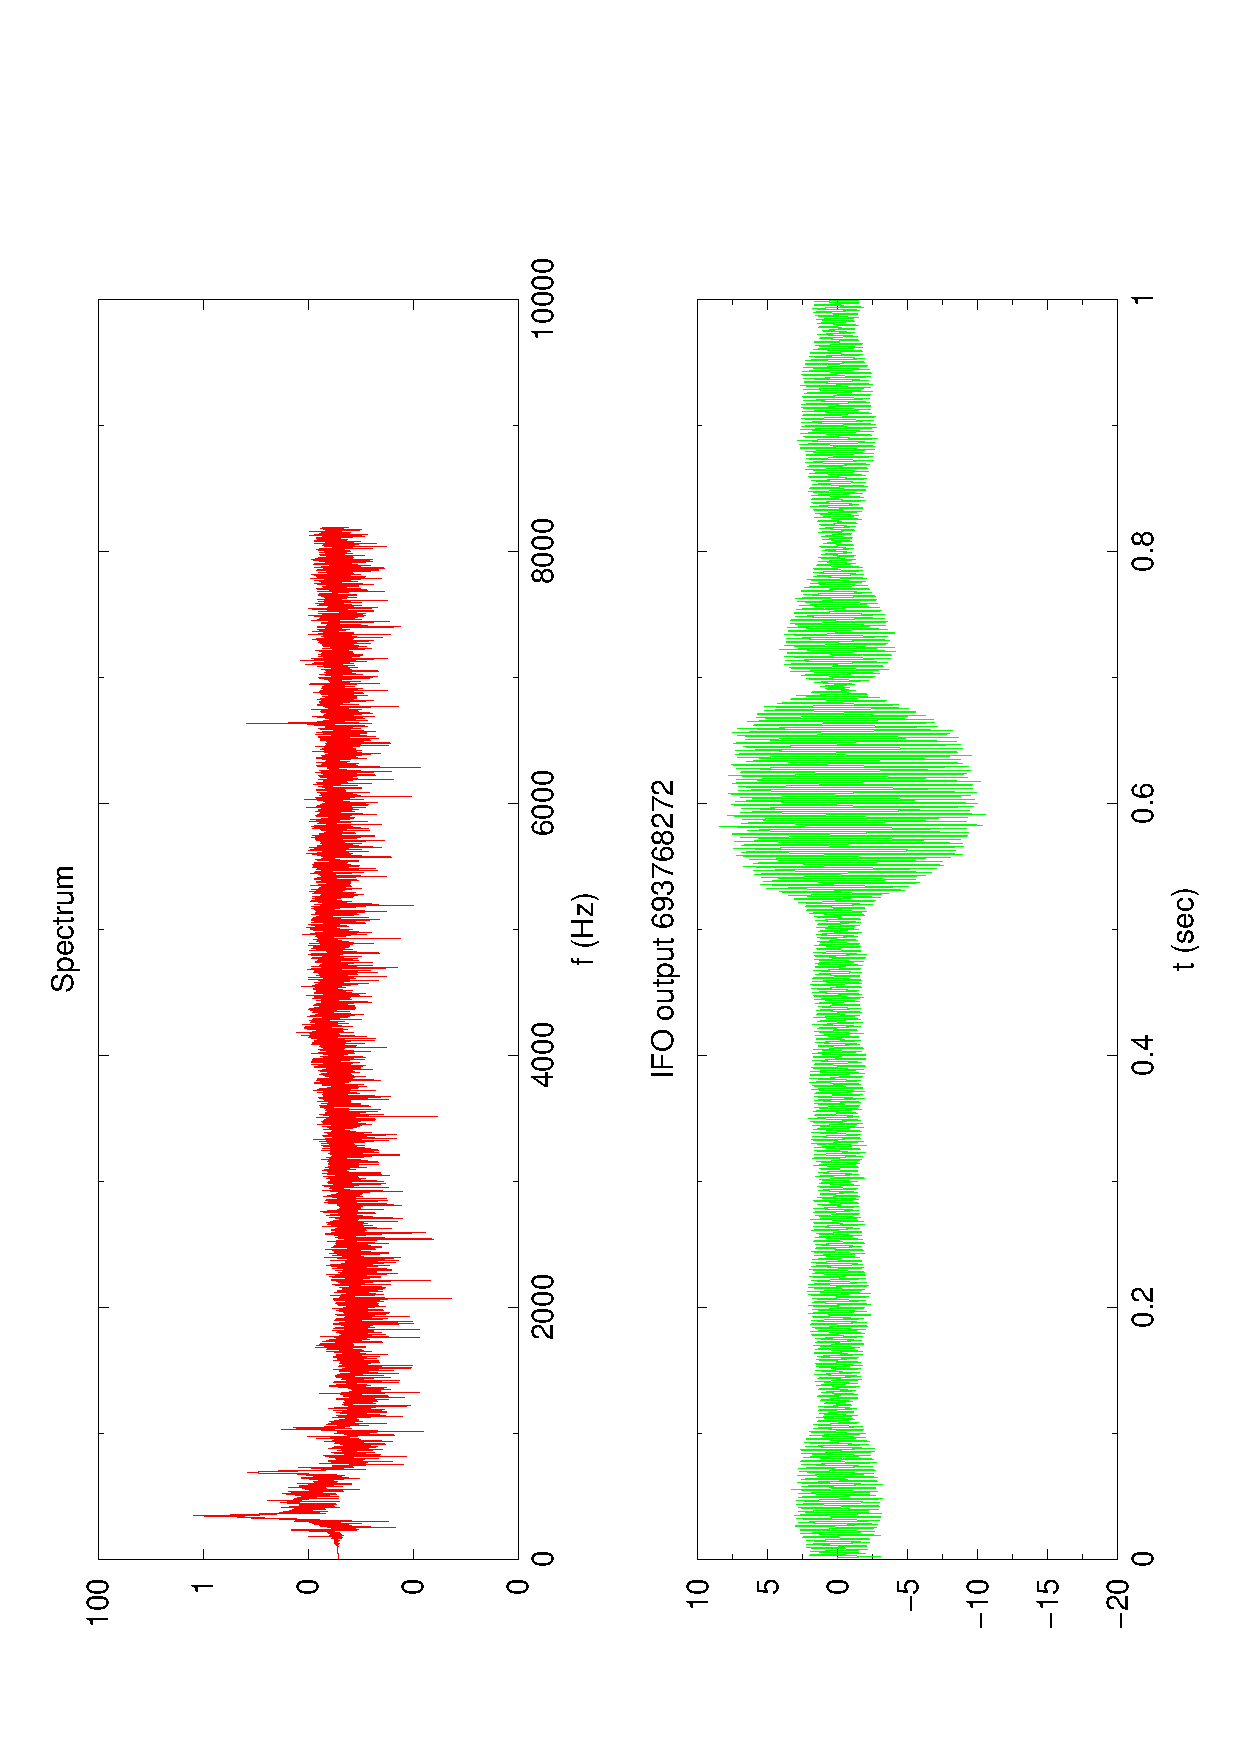
\includegraphics[angle=-90,width=400pt]{animate}
\end{center}
\end{figure}

\item[Author]
Bruce Allen and Patrick Brady

\end{entry}

\include{calibration}
\clearpage

\section{Findchirp Programs}
\label{section:findchirp}

This section of \textsc{LALApps} contains programs part of the findchirp packages
related to inspiral studies. 



\section{Program \texttt{lalapps\_inspiral}}
\label{program:lalapps-inspiral}
\idx[Program]{lalapps\_inspiral}

\begin{entry}
\item[Name]
\verb$lalapps_inspiral$ --- stand alone inspiral search code

\item[Synopsis] \prog{lalapps\_inspiral} \newline \hspace*{0.5in}
[\option{--help}] \newline \hspace*{0.5in} 
[\option{--verbose}] \newline \hspace*{0.5in} 
[\option{--version}] \newline \hspace*{0.5in}
[\option{--debug-level}~\parm{LEVEL}] \newline \hspace*{0.5in} 
[\option{--user-tag}~\parm{STRING}] \newline \hspace*{0.5in}           
[\option{--ifo-tag}~\parm{STRING}] \newline \hspace*{0.5in}
\option{--debug-level}~\parm{LEVEL}] \newline \hspace*{0.5in}
\option{--gps-start-time}~\parm{seconds} \newline \hspace*{0.5in}           
\option{--gps-start-time-ns}~\parm{nanoseconds} \newline \hspace*{0.5in}        
\option{--gps-end-time}~\parm{seconds} \newline \hspace*{0.5in}            
\option{--gps-end-time-ns}~\parm{nanoseconds} \newline \hspace*{0.5in}          
\option{--pad-data}~\parm{seconds} \newline \hspace*{0.5in}                  
[\option{--slide-time}~\parm{seconds}] \newline \hspace*{0.5in}              
[\option{--slide-time-ns}~\parm{seconds}] \newline \hspace*{0.5in}           
[\option{--glob-frame-data}] \newline \hspace*{0.5in}            
[\option{--frame-type}~\parm{tag}] \newline \hspace*{0.5in}           
\option{--frame-cache} \newline \hspace*{0.5in}                   
\option{--calibration-cache}~\parm{file} \newline \hspace*{0.5in}      
\option{--channel-name}~\parm{channel} \newline \hspace*{0.5in}           
\option{--calibrated-data}~\parm{type} \newline \hspace*{0.5in}        
[\option{--geo-high-pass-freq}~\parm{frequency}] \newline \hspace*{0.5in}      
[\option{--geo-high-pass-order}~\parm{order}] \newline \hspace*{0.5in}     
[\option{--geo-high-pass-atten}~\parm{attenuation}] \newline \hspace*{0.5in}     
[\option{--injection-file}~\parm{file}] \newline \hspace*{0.5in}       
[\option{--inject-overhead} \newline \hspace*{0.5in}             
\option{--bank-file}~\parm{file} \newline \hspace*{0.5in}             
\option{--minimal-match}~\parm{m} \newline \hspace*{0.5in}             
[\option{--start-template}~\parm{n}] \newline \hspace*{0.5in}          
[\option{--stop-template}~\parm{n}] \newline \hspace*{0.5in}           
\option{--sample-rate}~\parm{frequency} \newline \hspace*{0.5in}               
\option{--resample-filter}~\parm{type} \newline \hspace*{0.5in}        
\option{--disable-high-pass} \newline \hspace*{0.5in}             
\option{--enable-high-pass}~\parm{frequency} \newline \hspace*{0.5in}          
\option{--high-pass-order}~\parm{order} \newline \hspace*{0.5in}           
\option{--high-pass-attenuation}~\parm{attenuation} \newline \hspace*{0.5in}    
\option{--spectrum-type}~\parm{type} \newline \hspace*{0.5in}          
\option{--segment-length}~\parm{n} \newline \hspace*{0.5in}            
\option{--number-of-segments}~\parm{n} \newline \hspace*{0.5in}        
\option{--segment-overlap}~\parm{n} \newline \hspace*{0.5in}          
\option{--low-frequency-cutoff}~\parm{frequency} \newline \hspace*{0.5in}     
\option{--inverse-spec-length}~\parm{seconds} \newline \hspace*{0.5in}      
\option{--dynamic-range-exponent}~\parm{x} \newline \hspace*{0.5in}    
\option{--approximant}~\parm{approximant} \newline \hspace*{0.5in}            
\option{--chisq-bins}~\parm{number} \newline \hspace*{0.5in}                
\option{--snr-threshold}~\parm{rho-value} \newline \hspace*{0.5in}           
\option{--chisq-threshold}~\parm{chisq-value} \newline \hspace*{0.5in}          
\option{--enable-event-cluster} \newline \hspace*{0.5in}          
\option{--disable-event-cluster} \newline \hspace*{0.5in}        
\option{--enable-output} \newline \hspace*{0.5in}                
\option{--disable-output} \newline \hspace*{0.5in}                
[\option{--trig-start-time}~\parm{seconds}] \newline \hspace*{0.5in}       
[\option{--trig-end-time}~\parm{seconds}] \newline \hspace*{0.5in}        
[\option{--gaussian-noise}~\parm{var}] \newline \hspace*{0.5in}        
[\option{--random-seed}~\parm{seed}] \newline \hspace*{0.5in}          
[\option{--bank-simulation}~\parm{n}] \newline \hspace*{0.5in}      
[\option{--sim-approximant}~\parm{approximant}] \newline \hspace*{0.5in}      
[\option{--sim-minimum-mass}~\parm{mass}] \newline \hspace*{0.5in}        
[\option{--sim-maximum-mass}~\parm{mass}] \newline \hspace*{0.5in}        
[\option{--data-checkpoint}] \newline \hspace*{0.5in}             
[\option{--checkpoint-path}~\parm{path}] \newline \hspace*{0.5in} 
[\option{--output-path}~\parm{path}] \newline \hspace*{0.5in}          
[\option{--write-raw-data}] \newline \hspace*{0.5in}              
[\option{--write-filter-data}] \newline \hspace*{0.5in}           
[\option{--write-response}] \newline \hspace*{0.5in}              
[\option{--write-spectrum}] \newline \hspace*{0.5in}              
[\option{--write-snrsq}] \newline \hspace*{0.5in}                 
[\option{--write-chisq}] \newline \hspace*{0.5in}                 

\item[Description] 
\prog{lalapps\_inspiral} is a stand alone code for performing matched filtering for inspiral signals on LIGO 
or GEO data for gravitational wave signals and Monte Carlo analysis; it also has the capability of doing software signal injections on the data. 

\item[Options]\leavevmode
\begin{entry}
\item[\option{--help}] Display a brief usage summary.

\item[\option{--verbose}] print progress information

\item[\option{--debug-level}~\parm{level}] set the LAL debug level to 
LEVEL. For example: 1 :developer, 33 :production.

\item[\option{user-tag}~\parm{string}] set the process-params usertag to 
string

\item[\option{--ifo-tag}~\parm{string}] set the ifotag to string - for 
file naming

\item[\option{--gps-start-time}~\parm{seconds}] GPS second of data start 
time

\item[\option{--gps-start-time-ns}~\parm{nanoseconds}] GPS nanosecond of 
data start time

\item[\option{--gps-end-time}~\parm{seconds}] GPS second of data end 
time

\item[\option{--gps-end-time-ns}~\parm{nanoseconds}] GPS nanosecond of 
data end time

\item[\option{--pad-data}~\parm{seconds}] pad the data start and end time 
by 

\item[\option{--slide-time}~\parm{seconds}] slide data start epoch by 
seconds

\item[\option{--slide-time-ns}~\parm{seconds}] slide data start epoch by 
nanoseconds

\item[\option{--glob-frame-data}] glob *.gwf files in the pwd to obtain 
frame data

\item[\option{--frame-type}~\parm{tag}] input data is contained in frames 
of type tag

\item[\option{--frame-cache}~\parm{file}] obtain frame data from LAL 
frame cache 
 
\item[\option{--calibration-cache}~\parm{file}] obtain calibration from 
LAL frame cache 

\item[\option{--channel-name}~\parm{channel}] read data from 
interferometer channel 

\item[\option{--calibrated-data}~\parm{type}] calibrated data of type 
real-4 or real-8

\item[\option{--geo-high-pass-freq}~\parm{frequency}] high pass GEO data 
above F Hz using an IIR filter

\item[\option{--geo-high-pass-order}~\parm{order}] set the order of the 
GEO high pass filter to O

\item[\option{--geo-high-pass-atten}~\parm{attenuation}] set the
attenuation of the high pass filter to A

\item[\option{--injection-file}~\parm{file}] inject simulated inspiral 
signals from FILE

\item[\option{--inject-overhead}] inject signals directly overhead 
detector

\item[\option{--bank-file}~\parm{file}] read template bank parameters 
from FILE

\item[\option{--minimal-match}~\parm{m}] override bank minimal match with 
M (sets delta)

\item[\option{--start-template}~\parm{n}] start filtering at template 
number N in bank

\item[\option{--stop-template}~\parm{n}] stop filtering at template 
number N in bank

\item[\option{--sample-rate}~\parm{frequency}] filter data at F Hz, 
downsampling if necessary

\item[\option{--resample-filter}~\parm{type}] set resample filter to TYPE 
(ldas|butterworth)

\item[\option{--disable-high-pass}] turn off the IIR highpass filter

\item[\option{--enable-high-pass}~\parm{frequency}] high pass data above 
F Hz using an IIR filter

\item[\option{--high-pass-order}~\parm{order}] set the order of the high 
pass filter to O 

\item[\option{--high-pass-attenuation}~\parm{attenuation}] set the 
attenuation of the high pass filter to A

\item[\option{--spectrum-type}~\parm{type}] use PSD estimator TYPE 
(mean|median)

\item[\option{--segment-length}~\parm{n}] set data segment length to N 
points

\item[\option{--number-of-segments}~\parm{n}] set number of data segments 
to N

\item[\option{--segment-overlap}~\parm{n}] overlap data segments by N 
points

\item[\option{--low-frequency-cutoff}~\parm{frequency}] do not filter 
below F Hz

\item[\option{--inverse-spec-length}~\parm{seconds}] set length of 
inverse spectrum to T seconds

\item[\option{--dynamic-range-exponent}~\parm{x}] set dynamic range 
scaling to $2^X$ 

\item[\option{--approximant}~\parm{approximant}] approximant to be used. 
{TaylorF2|BCV} 

\item[\option{--chisq-bins}~\parm{number}] set number of chisq veto bins 
to P

\item[\option{--snr-threshold}~\parm{rho-value}] set signal-to-noise 
threshold to RHO

\item[\option{--chisq-threshold}~\parm{chisq-value}] threshold on $chi^2 
< X * ( p + rho^2 * delta^2 )$

\item[\option{--enable-event-cluster}] turn on maximization over chirp 
length

\item[\option{--disable-event-cluster}] turn off maximization over chirp 
length

\item[\option{--enable-output}] write the results to a LIGO LW XML file

\item[\option{--disable-output}] do not write LIGO LW XML output file

\item[\option{--trig-start-time}~\parm{gps-seconds}] only output triggers 
after GPS time SEC

\item[\option{--trig-end-time}~\parm{gps-seconds}] only output triggers 
before GPS time SEC

\item[\option{--gaussian-noise}~\parm{var}] replace data with gaussian 
noise of variance VAR

\item[\option{--random-seed}~\parm{seed}] set random number seed for
injections to SEED (urandom|integer)

\item[\option{--bank-simulation}~\parm{n}] perform N injections to test 
the template bank

\item[\option{--sim-approximant}~\parm{approximant}] set approximant of 
the injected waveform to APX

\item[\option{--sim-minimum-mass}~\parm{mass}] set minimum mass of bank 
injected signal to M

\item[\option{--sim-maximum-mass}~\parm{mass}] set maximum mass of bank
injected signal to M

\item[\option{--data-checkpoint}] checkpoint and exit after data is read 
in

\item[\option{--checkpoint-path}~\parm{path}] write checkpoint file under 
PATH

\item[\option{--output-path}] write output data to PATH

\item[\option{--write-raw-data}] write raw data to a frame file

\item[\option{--write-filter-data}] write data that is passed to filter 
to a frame

\item[\option{--write-response}] write the computed response function to 
a frame

\item[\option{--write-spectrum}] write the uncalibrated psd to a frame

\item[\option{--write-snrsq}] write the snr time series for each data 
segment

\item[\option{--write-chisq}] write the $r�2$ time series for each data 
segment


\end{entry}

\item[Example]
To run the program, type:
\begin{verbatim}
lalapps_inspiral \
--verbose \
--debug-level 33 \ 
--gps-start-time 73200096 \
--gps-end-time 732902144 \
--bank-file L1-TMPLTBANK-732900096-2048.xml \
--calibration-cache L-CAL-729273600-734367600.cache \ 
--frame-cache L1-732900096-2048.cache \
 --channel-name L1:LSC-AS_Q \
--snr-threshold 6.0 \
--chisq-threshold 5.0 \
--pad-data 8 \
--segment-length 1048576 \
--number-of-segments 15 \
--sample-rate 4096 \
--resample-filter ldas \
--enable-high-pass 100.0 \ 
--high-pass-order 8 \
--high-pass-attenuation 0.1 \ 
--spectrum-type median \
--low-frequency-cutoff 100.0 \ 
--approximant TaylorF2 \
--minimal-match 0.9 \
--segment-overlap 524288 \
--inverse-spec-length 16 \
--enable-event-cluster \
--dynamic-range-exponent 69.0 \ 
--chisq-bins 15 \
--enable-output \
--write-snr \
--write-chisq \
\end{verbatim} 





\item[Author] Duncan Brown 
\end{entry}

\documentclass{article}
\usepackage{fullpage}
\usepackage{kcannon0}

\DeclareGraphicsRule{.fig.pdf}{pdf}{.fig.pdf}{}


\newcommand\lal{\textsc{lal}}
\newcommand\lalapps{\textsc{lalapps}}
\newcommand\ligotools{\textsc{ligotools}}

\newcommand{\prog}[1]{\texttt{#1}}
\newcommand{\function}[1]{\texttt{#1}}
\newcommand{\option}[1]{\texttt{#1}}
\newcommand{\parm}[1]{$<$\textit{#1}$>$}


\newenvironment{entry}%
  {\begin{list}{}{\renewcommand{\makelabel}[1]%
    {\parbox[b]{\labelwidth}{\makebox[0pt][l]{\textbf{##1}}\\}}%
    \setlength{\labelwidth}{1em}%
    \setlength{\labelsep}{1em}%
    \setlength{\leftmargin}{2em}%
    \setlength{\topsep}{\medskipamount}%
    \setlength{\itemsep}{\medskipamount}%
    \setlength{\parsep}{\medskipamount}%
    \setlength{\listparindent}{0pt}}}
  {\end{list}}



\title{Burst Search Programs}
\author{Patrick Brady, Duncan Brown, Kipp Cannon, Saikat Ray-Majumder}
\date{2007-7-6}


\begin{document}
\maketitle

 
%%%%%%%%%%%%%%%%%%%%%%%%%%%%%%%%%%%%%%%%%%%%%%%%%%%%%%%%%%%%%%%%%%%%%
% RUNNING A PIPELINE
%%%%%%%%%%%%%%%%%%%%%%%%%%%%%%%%%%%%%%%%%%%%%%%%%%%%%%%%%%%%%%%%%%%%%
\section{Running the power code under Condor}
\label{subsection:running_power}

%
% FIXME: this section is obsolete
%

This section is under construction!


%%%%%%%%%%%%%%%%%%%%%%%%%%%%%%%%%%%%%%%%%%%%%%%%%%%%%%%%%%%%%%%%%%%%%%%%%%%%%%%
% subsection: power pipeline script
%%%%%%%%%%%%%%%%%%%%%%%%%%%%%%%%%%%%%%%%%%%%%%%%%%%%%%%%%%%%%%%%%%%%%%%%%%%%%%%
\section{Program \prog{lalapps\_power\_pipe}}
\label{program:lalapps-power-pipe}

\begin{entry}

\item[Name]
\prog{lalapps\_power\_pipe} --- builds a one/two/three interferometer excess-power
search DAG   

\item[Synopsis]
\prog{lalapps\_power\_pipe} \newline \hspace*{0.5in}
[\option{-h, --help}] \newline \hspace*{0.5in}
[\option{-v, --version}] \newline \hspace*{0.5in}
[\option{-u, --user-tag}~\parm{tag}] \newline \hspace*{0.5in}
[\option{-d, --datafind}] \newline \hspace*{0.5in}
[\option{-r, --power}] \newline \hspace*{0.5in}
[\option{-H, --ifo\_h1}] \newline \hspace*{0.5in}
[\option{-K, --ifo\_h2}] \newline \hspace*{0.5in}
[\option{-L, --ifo\_l}] \newline \hspace*{0.5in}
[\option{-c, --makeinjfiles}] \newline \hspace*{0.5in}
[\option{-j, --injections}~\parm{injection type}] \newline \hspace*{0.5in}
[\option{-m, --mdcinjections}] \newline \hspace*{0.5in}
[\option{-b, --coincidence}] \newline \hspace*{0.5in}
[\option{-t, --triplecoincidence}] \newline \hspace*{0.5in}
[\option{-s, --timeslides}] \newline \hspace*{0.5in}
[\option{-p, --playground-only}] \newline \hspace*{0.5in}
[\option{-P, --priority}~\parm{prio}] \newline \hspace*{0.5in}
\option{-f, --config-file}~\parm{file} \newline \hspace*{0.5in}
\option{-l, --log-path}~\parm{path}

\item[Description] 
\prog{lalapps\_power\_pipe} builds an excess power search DAG suitable for
running at the various LSC Data Grid sites.   The script requires a
configuration file.   An example file can be found in
\texttt{\$LALPREFIX/share/lalapps/power\_pipe.ini}.   Arguments to be
passed to the search code are supplied in this file and used the DAG
construction.  This is a standard python format configuration file.

\item[Options]\leavevmode
\begin{entry}

\item[\option{--help}] Prints the usage information

\item[\option{--user-tag} \parm{tag}]   The tag for the job.  This will
override the value set in the ini file

\item[\option{--datafind}] run LSCdataFind as part of the DAG to create the
cache files for each science segment

\item[\option{--power}] run \prog{lalapps\_power} on the data.  To run
the power jobs one has to specify the ifo or the combination of ifos.  This
can be specified by a combination of the options \option{--ifo\_h1},
 \option{--ifo\_h2} and \option{--ifo\_l}.  

\item[\option{--ifo\_h1}] run \prog{lalapps\_power} on the data from H1

\item[\option{--ifo\_h2}] run \prog{lalapps\_power} on the data from H2

\item[\option{--ifo\_l}] run \prog{lalapps\_power} on the data from L1

If one wants to run on both H1 and H2 data then the options \option{--ifo\_h1}
and \option{--ifo\_h2} have to be specified with \option{--power} and 
similarly for other combinations.  For example if one then wants to run on 
all of H1,  H2 and L1 data then all the three options,  \option{--ifo\_h1},
 \option{--ifo\_h2},  \option{--ifo\_l} have to be specified with the 
\option{--power}.

\item[\option{--makeinjfiles}] run \prog{lalapps\_binj} or 
\prog{lalapps\_bbhinj} to generate the injection files for each science
segment. These files are then used by the power jobs as the injection
parameter files.  However,  specifying this option tells the dag to 
create the injection files only.  Whether to perform the injections or not
is specified by the option \option{--injections} along with the type of 
waveform we would inject.    

\item[\option{--injections} \parm{type}] When this option is specifed 
simulated waveforms are injected to the data.  To use this option either
the injection files have to be in the directory or has to be used along with
\option{--makeinjfiles}.  The type of the injections also has to be specified 
with this option. The valid types are \texttt{burst, inspiral, burstandinspiral
and sim}.  \texttt{burst} indicates burst waveforms, \texttt{inspiral} 
indicates inspiral waveforms, \texttt{burstandinspiral} indicates both
burst and inspiral waveforms are to be injected and \texttt{sim} indicates
waveforms like warren,  kudu.

\item[\option{--mdcinjections}] run jobs with MDC injections      

\item[\option{--coincidence}] run \prog{lalapps\_burca} doing double 
coincidence analysis.  However note that to use this option either
two of the ifo options have to be used or the trigger files from two ifos 
have to be in the directory.

\item[\option{--triplecoincidence}] triple coincidence analysis is performed.  
As in double coincidence this option is to be used
either with the three ifo options or the trigger files from three ifos have
to be in the directory.

\item[\option{--timeslides}] perform the timeslide analysis. Timeslides
are currently performed only between sites, i.e. between Hanford and 
Livingstone. So to use this option either \option{--ifo\_h1} or 
\option{--ifo\_h2} or both have to be used with \option{--ifo\_l} or the 
trigger files have to be in the directory. 

\item[\option{--priority} \parm{prio}] run jobs with condor priority
\parm{prio}.

\item[\option{--config-file} \parm{file}] use configuration file
\parm{file}.

\item[\option{--log-path} \parm{path}] directory to write condor log file

\end{entry}


\item[Example]
To run the program which will do the datafind,  power nodes on the H1
and L1 data with simulated injections doing a double coincidence analysis
using the power\_pipe.ini file(which should be in the directory) type:
\begin{verbatim}
lalapps_power_pipe -f power_pipe.ini -d -r -H -L -b -c -j sim -l /people/saikat/log/
\end{verbatim}

\item[Author]
Duncan Brown, Patrick Brady and Saikat Ray-Majumder
\end{entry}


%%%%%%%%%%%%%%%%%%%%%%%%%%%%%%%%%%%%%%%%%%%%%%%%%%%%%%%%%%%%%%%%%%%%%%%%%%%%%%%
% section: power code
%%%%%%%%%%%%%%%%%%%%%%%%%%%%%%%%%%%%%%%%%%%%%%%%%%%%%%%%%%%%%%%%%%%%%%%%%%%%%%%
\section{Program \prog{lalapps\_power}}
\label{program:lalapps-power}

\begin{entry}

\item[Name]
\prog{lalapps\_power} --- performs excess power analysis on real or
simulated data.

\item[Synopsis]
\prog{lalapps\_power} \newline \hspace*{0.5in}
\option{--bandwidth}~\parm{Hz} \newline \hspace*{0.5in}
[\option{--burstinjection-file}~\parm{file name}] \newline \hspace*{0.5in}
[\option{--calibrated-data}~\parm{high pass frequency}] \newline \hspace*{0.5in}
[\option{--calibration-cache}~\parm{cache file}] \newline \hspace*{0.5in}
\option{--channel-name}~\parm{string} \newline \hspace*{0.5in}
\option{--confidence-threshold}~\parm{threshold} \newline \hspace*{0.5in}
[\option{--debug-level}~\option{info|warn|error|off}] \newline \hspace*{0.5in}
[\option{--dump-diagnostics~\parm{XML filename}}] \newline \hspace*{0.5in}
\option{--filter-corruption}~\parm{samples} \newline \hspace*{0.5in}
\option{--frame-cache}~\parm{cache file} \newline \hspace*{0.5in}
[\option{--gaussian-noise-rms}~\parm{RMS}] \newline \hspace*{0.5in}
\option{--gps-end-time}~\parm{seconds} \newline \hspace*{0.5in}
\option{--gps-start-time}~\parm{seconds} \newline \hspace*{0.5in}
[\option{--help}] \newline \hspace*{0.5in}
\option{--high-pass}~\parm{Hz} \newline \hspace*{0.5in}
[\option{--inspiralinjection-file}~\parm{file name}] \newline \hspace*{0.5in}
\option{--low-freq-cutoff}~\parm{Hz} \newline \hspace*{0.5in}
[\option{--max-event-rate}~\parm{Hz}] \newline \hspace*{0.5in}
\option{--max-tile-bandwidth}~\parm{Hz} \newline \hspace*{0.5in}
\option{--max-tile-duration}~\parm{seconds} \newline \hspace*{0.5in}
[\option{--mdc-cache}~\parm{cache file}] \newline \hspace*{0.5in}
[\option{--mdc-channel}~\parm{channel name}] \newline \hspace*{0.5in}
[\option{--output}~\parm{file name}] \newline \hspace*{0.5in}
\option{--psd-average-method}~\parm{method} \newline \hspace*{0.5in}
\option{--psd-average-points}~\parm{samples} \newline \hspace*{0.5in}
[\option{--ram-limit}~\parm{MebiBytes}] \newline \hspace*{0.5in}
\option{--resample-rate}~\parm{Hz} \newline \hspace*{0.5in}
[\option{--sim-cache}~\parm{cache file}] \newline \hspace*{0.5in}
[\option{--sim-seconds}~\parm{sec.s}] \newline \hspace*{0.5in}
[\option{--siminjection-file}~\parm{injection file}] \newline \hspace*{0.5in}
[\option{--seed}~\parm{seed}] \newline \hspace*{0.5in}
\option{--target-sample-rate}~\parm{Hz} \newline \hspace*{0.5in}
\option{--tile-stride-fraction}~\parm{fraction} \newline \hspace*{0.5in}
[\option{--enable-over-whitening}] \newline \hspace*{0.5in}
[\option{--user-tag}~\parm{comment}] \newline \hspace*{0.5in}
\option{--window-length}~\parm{samples} \newline \hspace*{0.5in}

\item[Description] 
\prog{lalapps\_power} performs an excess power analysis on real or
simulated data.  Consider searching for signals with the following
properties:
\begin{itemize}
\item Maximum signal time duration $T=2^a$ seconds where $a$ is a positive
or negative integer;  the sampling rate of the data stream is taken
assummed $\mbox{\texttt{srate}} = 2^b$ Hz.

\item The frequency band of the signal is between $f_{\mathrm{low}}$ Hz and
${f_{\mathrm{high}}}$ Hz.  Current versions of the code expect
${f_{\mathrm{high}}}-{f_{\mathrm{low}}}=2^d$ Hz where $d$ is an integer. 

\item Minimum time duration,

\item Minimum frequency bandwidth.
\end{itemize}

The input data for a search consists of LIGO/VIRGO \texttt{.gwf} frame
files.  These files can be collected together in a single directory, or in
locations described via the LAL frame cache file mechanism.  The code can
be used for Monte-Carlo simulations to determine search efficiency by
providing a list of injections to be made;  this injections list must be in
LIGO lightweight format and can be generated using the \prog{lalapps\_binj}
program described in Sec.~\ref{program:lalapps-binj}. 

The output data is written as \verb|sngl_burst| triggers in LIGO
lightweight XML files.  The files are named according to a standardized
naming convention
\begin{quote}
\{IFO\}-POWER\_\{comment\}-\{GPS Start Time\}-\{duration\}.xml
\end{quote}
For example, if a search was run on the Hanford 4km interferometer and
generated triiggers starting at 731488397 and the triggers cover 33 seconds
after that time,  then the file name would be 
\begin{quote}
H1-POWER\_test\_this\_again-731488397-33.xml
\end{quote}
where the comment was ``test\_this\_again''.  Note that the comment should
not include spaces and should use underscores instead.

\item[Options]\leavevmode
\begin{entry}
\item[\option{--bandwidth} \parm{Hz}]
Set the bandwidth in which the search is to be performed.  This must be a
power of 2.

\item[\option{--burstinjection-file} \parm{file name}]
Use \parm{file name} as a LIGO lightweight XML file containing a list of
injections to be made.   The file should contain a \verb+sim_burst+ table
which is used to set information about the types of burst injections to be
made.  This file may be constructed by hand, the \verb+lalapps_binj+
program described in Section \ref{program:lalapps-binj}.

\item[\option{--calibrated-data} \parm{high pass frequency}]
When the \option{--calibrated-data} option is supplied, input time series
data is read as IEEE double-precision samples.  Calibrated data, for
example from the GEO detector, is stored in double-precision rather than
single-precision format.

This program uses IEEE single-precision internally, so double-precision
data must be quantized prior to processing.  It is typically necessary to
remove low-frequency noise from the signal prior to quantization in order
to reduce the loss of fidelity.  \parm{high pass frequency} sets the
cut-off frequency, in Hertz, of the high-pass filter applied to the time
series prior to quantization to single-precision.

\item[\option{--calibration-cache} \parm{cache file}]
Specify the location of calibration information.  \parm{cache file} gives
the path to a LAL-format frame cache file describing locations of
\texttt{.gwf} frame files that provide the calibration data ($\alpha$ and
$\beta$ coefficients) for the analysis.  Frame cache files are explained in
the ``framedata'' package in LAL.

\item[\option{--channel-name} \parm{string}]
Set the name of the data channel to analyze to \parm{string}.  This must
match the name of one of the data channels in the input frame files.  For
example, ``\verb|H2:LSC-AS_Q|''.

\item[\option{--confidence-threshold} \parm{threshold}]
Set the confidence threshold below which events should be discarded.  The
``confidence'' of an event is \(-\ln P(\text{event} | \text{stationary
Gaussian white noise})\), so an event with a confidence of 30 has a
probability of \(\ee^{-30}\) of being found in stationary Gaussian white
noise.  LIGO strain outputs are not stationary, and so a typical,
practical, threshold is 70 or higher.

\item[\option{--debug-level} \option{info|warn|error|off}]
Sets the level of verbosity:  \option{info} = print all messages,
\option{warn} = print only warnings and errors, \option{error} = print only
errors, and \option{off} = be silent.  The default value is \option{error}.

\item[\option{--dump-diagnostics \parm{XML filename}}]
Dump diagnostic snapshots of internal time and frequency series data to a
LIGO Light Weight XML file of the given name.  The file is overwritten.

\item[\option{--filter-corruption} \parm{samples}]
The input time series data is passed through a conditioning filter prior to
analysis.  Generally, the conditioning filter should be expected to corrupt
some amount of the beginning and end of the time series due to edge
effects.  This parameter tells the code how much data, in samples, should
be ignored from the start and end of the time series.  A reasonable value
is 0.5 seconds worth of data.

\item[\option{--frame-cache} \parm{cache file}]
Obtain the locations of input \texttt{.gwf} frame files from the LAL frame
cache file \parm{cache file}.  LAL frame cache files are explained in the
``framedata'' package in LAL and can be constructed by making calls to
\prog{LSCDataFind} on some systems.  One of \option{--frame-cache}, or
\option{--gaussian-noise-rms} must be specified.

\item[\option{--gaussian-noise-rms} \parm{RMS}]
If this parameter is provided instead of \option{--frame-cache}, then
Gaussian white noise will be synthesized and used as the input data.  One
of \option{--frame-cache}, or \option{--gaussian-noise-rms} must be
specified.

\item[\option{--gps-end-time} \parm{seconds}]
Set the GPS time up to which input data should be read to \parm{seconds}.
Non-integer values are permitted, but the fractional part must not contain
more than 9 digits (accurate to nanoseconds).

\item[\option{--gps-start-time} \parm{seconds}]
Set the GPS time from which to start reading input data to \parm{seconds}.
Non-integer values are permitted, but the fractional part must not contain
more than 9 digits (accurate to nanoseconds).

\item[\option{--help}]
Display a usage message and exit.

\item[\option{--high-pass} \parm{Hz}]
The input time series is high-pass filtered as part of the input data
conditioning.  This argument sets the cut-off frequency for this filter.
In older versions of the program, this frequency has hard-coded to be
\unit{10}{\hertz} below the lower bound of the frequency band being
searched or \unit{150}{Hz}, which ever was lower.

\item[\option{--inspiralinjection-file} \parm{file name}]
Use \parm{file name} as a LIGO lightweight XML file containing a list of inspiral
injections to be made.   The file should contain a \verb+sim_inspiral+ table
which is used to set information about the types of inspiral injections to be made.
This file may be constructed by hand, the
\verb+lalapps_bbhinj+ program described in the Inspiral package   

\item[\option{--low-freq-cutoff} \parm{Hz}]
Set the lowest frequency at which to search for gravitational waves to
\parm{Hz}.  This parameter is $f_{\mathrm{low}}$ from our description of
the desired signal parameters above.

\item[\option{--max-event-rate} \parm{Hz}]
Exit with a failure if the event rate, averaged over the entire analysis
segment, exceeds this limit.  This provides a safety valve to prevent the
code from filling up disks if the threshold is set improperly.  A value of
0 (the default) disables this feature.

\item[\option{--max-tile-bandwidth} \parm{Hz}]
This specifies the maximum frequency bandwidth (\(B\)) that a tile can
have.  This also fixes the minimum time duration of the tiles, $\Delta t =
1/B $.  This must be an integer power of 2.

\item[\option{--max-tile-duration} \parm{s}]
This specifies the maximum duration that a tile can have.  This also fixes
the minimum bandwidth of the tiles.  This must be an integer power of 2.

\item[\option{--mdc-cache} \parm{cache file}]
Use \parm{cache file} as a LAL format frame cache file describing the
locations of MDC frames to be used for injections.

\item[\option{--mdc-channel} \parm{channel name}]
Use the data found in the channel \parm{channel name} in the MDC frames for
injections.

\item[\option{--output} \parm{file name}]
Set the name of the LIGO Light Weight XML file to which results will be
written.  The default is
``\parm{instrument}\_POWER\_\parm{comment}-\parm{start}-\parm{duration}.xml''.
Where \parm{instrument} is derived from the name of the channel being
analyzed, and \parm{comment} is obtained from the command line.
\parm{start} is the integar part of the GPS start time from the command
line, and \parm{duration} is the difference of the integer parts of the
GPS start and end times from the command line.

\item[\option{--psd-average-method} \parm{method}]
Set the averaging method used in determining the average power spectral
density to \parm{method}.  This can be one of ``useMean'', or
``useMedian''.

\item[\option{--psd-average-points} \parm{samples}]
Use \parm{samples} samples from the input time series to estimate the
average power spectral density of the detector's noise.  The average PSD is
used to whiten the data prior to applying the excess power statistic.  The
number of samples used for estimating the average PSD must be commensurate
with the analysis window length and analysis window spacing --- i.e.\ an
integer number of analysis windows must fit in the data used to estimate
the average PSD --- however this program will automatically round the
actual number of samples used down to the nearest integer for which this is
true.  This elliminates the need of the user to carefully determine a valid
number for this parameter, allowing him/her to instead select a number that
matches the observed length of time for which the instrument's noise is
stationary.

\item[\option{--ram-limit} \parm{MebiBytes}]
The start and stop GPS times may encompass a greater quantity of data than
can be analyzed at once due to RAM limitations.  This parameter can be used
to tell the code how much RAM, in MebiBytes, is available on the machine,
which it then uses to heursitically guess at a maximum time series length
that should be read.  The code then loops over the input data, processing
it in chunks of this size, until it has completed the analysis.  If this
parameter is not supplied, then the entire time series for the segment
identified by the GPS start and end times will be loaded into RAM.

\item[\option{--resample-rate} \parm{Hz}]
The sample frequency to which the data should be resampled prior to
analysis.  This must be a power of 2 in the range \unit{2}{\hertz} to
\unit{16386}{\hertz} inclusively.

\item[\option{--seed} \parm{seed}]
When synthesizing Gaussian white noise with \option{--gaussian-noise-rms},
this options can be optionally used to set the random number generator's
seed.

\item[\option{--target-sample-rate} \parm{Hz}]
Down-convert the input data stream to a sample rate of \parm{Hz} samples
per second prior to analysis.  This can be used to reduce the number of CPU
cycles required to analyze a given quantity of input data.  \emph{Note:}
All other parameters are given with respect to \emph{this} sample rate.
For example, the number of samples used to estimate the average PSD as
given by \option{--psd-average-points} refers to the time series following
data rate down-conversion.

\item[\option{--tile-stride-fraction} \parm{fraction}]
This parameter controls the amount by which adjacent time-frequency tiles
of the same size overlap one-another.  This numeric parameter must be \(=
2^{-n}\), where \(n \in \mathrm{Integers}\).  A reasonable value is 0.5,
which causes each tile to overlap its neighbours in time by \(\frac{1}{2}\)
its duration and in frequency by \(\frac{1}{2}\) its bandwidth.

\item[\option{--enable-over-whitening}]
Turn on over whitening.  The channel filters used to construct the
time-frequency plane will be weighted by the inverse of the noise power
spectral density, causing the pixels in the time-frequency plane to be
constructed preferentially from low-noise frequency bins.

\item[\option{--user-tag} \parm{comment}]
Set the user tag to the string \parm{comment}.  This string must not
contain spaces or dashes (``-'').  This string will appear in the name of
the file to which output information is written, and is recorded in the
various XML tables within the file.

\item[\option{--window-length} \parm{samples}]
Set the number of samples to use for an analysis window to \parm{samples}.
Only the central half of the window will be analyzed, the first quarter and
last quarter of the window are used as padding to avoid corruption at
certain stages of the analysis.  For example, if you wish the code to
analyze the data in 1 second windows, you need to set this parameter to the
number of samples corresponding to 2 seconds of data.  This parameter must
be a power of 2.

\end{entry}


\item[Example]
To run the program, type:
\begin{verbatim}
lalapps_power \
--bandwidth 2048 \
--calibrated-data 40.0 \
--channel-name "H1:LSC-STRAIN" \
--debug-level info \
--enable-over-whitening \
--filter-corruption 4096 \
--frame-cache H-754008315-754008371.cache \
--gps-end-time 754008363 \
--gps-start-time 754008323 \
--high-pass 60.0 \
--low-freq-cutoff 70.0 \
--max-event-rate 10000 \
--psd-average-method useMedian \
--psd-average-points 274432 \
--ram-limit 1024 \
--resample-rate 8192 \
--tile-stride-fraction 0.5 \
--user-tag testing \
--window-length 16384
\end{verbatim}
For this to succeed, the current directory must contain the file
\texttt{H-754008315-754008931.cache} describing the locations of the
\texttt{.gwf} frame files containing the channel \verb|H1:LSC-STRAIN|
spanning the GPS times 754008323.0 s through 754008363.0 s.

\item[Authors]
Patrick Brady, Saikat Ray-Majumder and Kipp Cannon.  
\end{entry}

\subsection{Algorithmic Implementation}


\subsubsection{Overview}

The Excess Power search method is motivated by the classical theory of
signal detection in Gaussian noise.  The method is the optimal search
strategy~\cite{Anderson:2000yy} having only knowledge of the time duration
and frequency band of the expected signal,  but having no other information
about the power distribution in advance of detection.

The algorithm amounts to projecting the data onto a basis of test
functions, each of which is a prototype for the waveforms being sought in
the data.  The projection procedure is the following.  The input time
series is passed through a comb of frequency-domain filters, generating
several output time series, one each for a number of frequency channels.
Summing the squares of the samples in any one of these channels amounts to
summing the ``energy'' in the corresponding frequency band.  Summing only
the samples from a range of times produces a number that is interpreted as
the energy in that frequency band for that period of time --- the energy in
a time-frequency tile whose bandwidth is that of the frequency channel, and
whose duration is the length of the sum.

The search is a multi-resolution search, so tiles of many different
bandwidths and durations are scanned.  For performance purposes, only a
single frequency channel decomposition is used.  ``Virtual'' wide bandwidth
channels are constructed by summing the samples from multiple channels, and
correcting for the overlap between adjacent channel filters.

Once the energy in a tile has been measured, a threshold is applied to
select the ``important'' tiles.  The quantity thresholded on is the
probability of measuring at least that much energy in a tile with that
bandwidth and that duration in Gaussian noise.  The procedure employed to
assess this probability is to first whiten and normalize the data, to
transform it into what is then assumed to be stationary white unit-variance
Gaussian noise, and then read off the probability of the observed energy
from a theoretical distribution derived from that assumption.


\subsubsection{The Whitening Procedure}

Consider a discretely-sampled time-series of \(N\) samples, \(s_j\) where
\(0 \leq j < N\) and the sample period is \(\Delta t\).  Much of the signal
processing to be described below is done in the frequency domain, so the
first step is to multiply the time series by a window function, \(w_{j}\),
tapering it to 0 at the start and end to reduce the noise arising from the
data's aperiodicity at its boundary.  The mean square of the tapering
window's samples is
\begin{equation}
\sigma_{w}^{2}
   = \frac{1}{N} \sum_{j = 0}^{N - 1} w_{j}^2.
\end{equation}
Following multiplication by the tapering window, the data is Fourier
transformed to the frequency domain.  The complex amplitude of the
frequency bin \(k\) is
\begin{equation}
\tilde{s}_{k}
   = \frac{\Delta t}{\sigma_{w}} \sum_{j = 0}^{N - 1} w_{j} s_{j} \ee^{-2
   \pi \aye j k / N},
\end{equation}
where \(0 \leq k < N\).  The frequency bins \(\lfloor N / 2 \rfloor < k <
N\) correspond to negative frequency components, and are not stored because
the input time series is real-valued and so the negative frequency
components are redundant (they are the complex conjugates of the positive
frequency components).  For the non-negative frequencies, bin \(k\)
corresponds to frequency
\begin{equation}
f_{k}
   = k \Delta f,
\end{equation}
where the bin spacing is \(\Delta f = (N \Delta t)^{-1}\).  Defining the
power spectral density as
\begin{equation}
P_{k}
   = \Delta f \mean{\magnitude{\tilde{s}_{k}}^{2} + \magnitude{\tilde{s}_{N
   - k}}^{2}}
   = 2 \Delta f \mean{\magnitude{\tilde{s}_{k}}^{2}},
\end{equation}
for \(0 \leq k < \lfloor N / 2 \rfloor\), the ``whitened'' frequency series
is
\begin{equation}
\hat{s}_{k}
   = \sqrt{\frac{2 \Delta f}{P_{k}}} \tilde{s}_{k}
\end{equation}
so that
\begin{equation}
\label{eqn3}
\mean{\magnitude{\hat{s}_{k}}^2}
   = 1.
\end{equation}
The definition of the power spectral density is such that
\begin{align}
\mean{s_{j}^{2}}
   & = \frac{1}{N^{2} \Delta t^{2}} \sum_{k = 0}^{N - 1} \sum_{k' = 0}^{N -
   1} \mean{\tilde{s}_{k} \conj{\tilde{s}}_{k'}} \ee^{2 \pi \aye j (k - k')
   / N}
   \\
   & = \frac{1}{2 N \Delta t} \sum_{k = 0}^{N - 1} P_{k},
\end{align}
when the frequency components are independent (the input time series is a
stationary process).

If the original time series is stationary Gaussian noise, this construction
makes each frequency bin's real and imaginary parts Gaussian random
variables with variances of 0.5.  The definition of the power spectral
density and of the Fourier transform shown above both match those of the
LIGO Algorithm Library, as documented in LIGO-T010095-00-Z.  Figure
\ref{fig:shistogram} shows the distribution of the real and imaginary
components of \(\hat{s}_{k}\) obtained from a sample of \(h(t)\) taken from
the LIGO L1 instrument during S4.
\begin{figure}
\begin{center}
\resizebox{5.5in}{!}{\includegraphics{figures/sk_histogram.png}}
\end{center}
\caption{The distribution of the real and imaginary components of
\(\hat{s}_{k}\) obtained from a sample of \(h(t)\) taken from the LIGO L1
instrument during S4.  The aparent bias away from the expected
normalization (actually non-Gaussianity) and the two horn features, are the
result of correlations between the power spectrum and the data.  Recall
that the power spectrum is estimated from the same data it is used to
whiten.}
\label{fig:shistogram}
\end{figure}

If the input time series is a stationary random process, then the
components of its Fourier transform are uncorrelated, and we would find
that \(\mean{\hat{s}_{k} \conj{\hat{s}}_{k'}} = \delta_{k k'}\).  However,
because we have windowed the time series (which is equivalent to convolving
its Fourier transform with that of the window), the frequency components
are now correlated.  We can compute \(\mean{\hat{s}_{k}
\conj{\hat{s}}_{k'}}\) by assuming the whitened time series consists of
independently-distributed random variables, because then the
Wiener-Khinchin theorem tells us that its two-point spectral correlation
function is the Fourier transform of its variance which we'll assume is
proportional to the square of the tapering window function.  Therefore,
\begin{equation}
\mean{\hat{s}_{k} \conj{\hat{s}}_{k'}}
   \propto \sum_{j = 0}^{N - 1} w_{j}^{2} \ee^{-2 \pi \aye j (k - k') / N}.
\end{equation}
The proportionality constant is obtained from \eqref{eqn3}, which tells us
that
\begin{equation}
\label{eqn4}
\mean{\hat{s}_{k} \conj{\hat{s}}_{k'}}
   = \frac{1}{\sigma_{w}^{2}} \sum_{j = 0}^{N - 1} w_{j}^{2} \ee^{-2 \pi
   \aye j (k - k') / N}.
\end{equation}
A comparison of this prediction to the observed two-point spectral
correlation in \(\hat{s}_{k}\) obtained from \(h(t)\) recorded at the LIGO
L1 instrument during S4 is shown in Figure \ref{fig:sksk}.
\begin{figure}
\begin{center}
\resizebox{5.5in}{!}{\includegraphics{figures/sksk.png}}
\end{center}
\caption{The two-point spectral correlation in the whitened data when a
Tukey window with 50\% flat top is used to taper the input time series.
The ``expected'' curve is what is expected in the limit of an average over
an infinite number of measurements.  Since a finite number of measurements
were made, a residual ``floor'' is expected, and it should go as
\((\text{number of measurements})^{-1/2}\).  Approximately 4 million
samples were averaged in each bin so the floor, which is
\(\mean{\hat{s}_{k} \conj{\hat{s}}_{k'}} \sim 2000^{-1}\), is consistent
with what is expected.}
\label{fig:sksk}
\end{figure}

The power spectral density is estimated using the median power at each
frequency for a number of overlapping segments.  The use of the median
avoids bias in the spectrum caused by the presence of a gravitational wave
or other large non-astrophysical transients present in any of the segments. 


\subsubsection{The Channel Filter}
\label{sec:channelfilter}

The choice of the channel filter is mostly irrelevant, except that it
correspond in some meaningful way to a particular frequency band.  We'll
denote the channel filter spanning frequencyes \(f_{1} \leq f_{k} < f_{2}\)
as \(\tilde{\Theta}_{k}(f_{1}, B)\), where the bandwidth of the filter is
\(B = f_{2} - f_{1}\).  If \(b\) is the bandwidth of the narrowest channel,
excess power achieves a multi-resolution search by computing only the
narrowest channels, and choosing
\begin{equation}
\tilde{\Theta}_{k}(f_{1}, n b)
   = \sum_{i = 0}^{n - 1} \Theta_{k}(f_{1} + i b, b),
\end{equation}
where \(B = n b\).  That is, the filters for wide band channels are chosen
to be the sums of adjacent filters from narrower bands.  The specific
choice made in excess power is to use Hann windows for the narrowest
channels.  The narrow channels are all the same width, and the Hann windows
are adjusted to be centred on their channel and extend over a range of
frequencies twice the width of the channel,
\begin{equation}
\tilde{\Theta}_{k}(f_{1}, b)
   \propto \begin{cases}
   \sin^{2} \frac{\pi}{2 b} (f_{k} - f_{1} + \frac{b}{2}), & f_{1} -
   \frac{b}{2} \leq f_{k} < f_{1} + \frac{3 b}{2} \\
   0, & \text{othewise}.
   \end{cases}
\end{equation}
In this way, when the filters for two adjacent channels are summed the
result is a Tukey window --- a window with a flat top in the middle and
\(\sin^{2}\) tapers at each end.

All windows are real-valued, so that they are phase preserving.  The
narrowest channel filters, the filters of bandwidth \(b\),  are normalized
so that
\begin{equation}
\label{eqn5}
\sum_{k = 0}^{N - 1} \sum_{k' = 0}^{N - 1} -1^{(k - k')} \mean{\hat{s}_{k}
\conj{\hat{s}}_{k'}} \conj{\tilde{\Theta}}_{k}(f_{1}, b)
\tilde{\Theta}_{k'}(f_{1}, b)
   = \frac{b}{\Delta f},
\end{equation}
where the two-point spectral correlation is given in \eqref{eqn4}.  The
reason for this choice will become clear later.  For convenience, let us
introduce the notation
\begin{equation}
\left\{ \tilde{X}, \tilde{Y} \right\}
   = \sum_{k = 0}^{N - 1} \sum_{k' = 0}^{N - 1} -1^{(k - k')}
   \mean{\hat{s}_{k} \conj{\hat{s}}_{k'}} \conj{\tilde{X}}_{k}
   \tilde{Y}_{k'},
\end{equation}
so
\begin{equation}
\left\{ \tilde{\Theta}(f_{1}, b), \tilde{\Theta}(f_{1}, b) \right\}
   = \frac{b}{\Delta f}.
\end{equation}
Notice that if the two-point spectral correlation is a Kroniker \(\delta\)
(the input data is not windowed), and the channel filter is flat,
\(\tilde{\Theta}_{k} = \tilde{\Theta}\), and spans the entire frequency
band from DC to Nyquist, \(b / \Delta f = N\), then the normalization would
lead to
\begin{equation}
\tilde{\Theta}
   = 1.
\end{equation}

In the LIGO Algorithm Library, the Fourier transforms of real-valued time
series contain only postive frequency components (the negative frequency
components being the complex conjugates of these), and so the channel
filters are also stored as only positive frequency components.  Since the
two-point spectral correlation function is usually strongly-peaked around
\(k - k' = 0\), and since the channel filters all go to zero far from the
DC and Nyquist components, in practice it is safe to sum over only the
positive frequency components, and require the sum to be
\begin{equation}
2 \sum_{k = 0}^{\lfloor N / 2 \rfloor + 1} \sum_{k' = 0}^{\lfloor N / 2
\rfloor + 1} -1^{(k - k')} \mean{\hat{s}_{k} \conj{\hat{s}}_{k'}}
\conj{\tilde{\Theta}}_{k}(f_{1}, b) \tilde{\Theta}_{k'}(f_{1}, b)
   = \frac{b}{\Delta f}.
\end{equation}
So the argument is that in practice this normalization is identical to
\eqref{eqn5}, but it is easier to implement because these are the only
components stored in memory.

For wide channels, channels formed by summing the filters from two or more
narrow channels, the ``magnitude'' of the channel filter will not be \(n b
/ \Delta f\).  For example,
\begin{equation}
\tilde{\Theta}_{k}(f_{1}, 2 b)
   = \tilde{\Theta}_{k}(f_{1}, b) + \tilde{\Theta}_{k}(f_{1} + b, b),
\end{equation}
and using the symmetry of \(\mean{\hat{s}_{k} \conj{\hat{s}}_{k'}}\) the
magnitude of this channel filter is found to be
\begin{align}
\left\{ \tilde{\Theta}(f_{1}, 2 b), \tilde{\Theta}(f_{1}, 2 b) \right\}
   & = \frac{2 b}{\Delta f} + 2 \left\{ \tilde{\Theta}(f_{1}, b),
   \tilde{\Theta}(f_{1} + b, b) \right\}.
\end{align}
The channel construction described above, with Hann windows for the
narrowest channels yielding Tukey windows for wider channels, allows us to
make the approximation that only adjacent channel filters have sufficient
overlap that their inner products are non-zero, and so the cross terms from
adjacent channels are the only ones that need to be accounted for.
Therefore, in general, a filter spanning \(n\) channels is
\begin{equation}
\tilde{\Theta}_{k}(f_{1}, n b)
   = \sum_{i = 0}^{n - 1} \tilde{\Theta}_{k}(f_{1} + i b, b),
\end{equation}
and its magnitude is
\begin{equation}
\left\{ \tilde{\Theta}(f_{1}, n b), \tilde{\Theta}(f_{1}, n b) \right\}
   = \frac{n b}{\Delta f} + 2 \sum_{i = 0}^{n - 2} \left\{
   \tilde{\Theta}(f_{1} + i b, b), \tilde{\Theta}(f_{1} + (i + 1) b, b)
   \right\}.
\end{equation}
Let us denote this magnitude as \(\mu^{2}(f_{1}, n b)\),
\begin{equation}
\label{eqn2}
\mu^{2}(f_{1}, n b)
   = \frac{n b}{\Delta f} + 2 \sum_{i = 0}^{n - 2} \sum_{k = 0}^{N - 1}
   \sum_{k' = 0}^{N - 1} -1^{(k - k')} \mean{\hat{s}_{k}
   \conj{\hat{s}}_{k'}} \tilde{\Theta}_{k}(f_{1} + i b, b)
   \conj{\tilde{\Theta}}_{k'}(f_{1} + (i + 1) b, b).
\end{equation}
When \(n = 1\), \(\mu^{2} = b / \Delta f\).

Figure \ref{fig:freqdomainfilter} illustrates the construction of a
\(\unit{16}{\hertz}\) channel filter from four \(\unit{4}{\hertz}\) channel
filters when \(\mean{\hat{s}_{k} \conj{\hat{s}}_{k'}} = \delta_{k k'}\).
\begin{figure}
\begin{center}
\includegraphics{figures/freqdomainfilter.pdf}
\end{center}
\caption{Summing narrow Hann channel filters to obtain wide-band Tukey
filters.}
\label{fig:freqdomainfilter}
\end{figure}
The \(\unit{16}{\hertz}\) channel filter has had its normalization adjusted
by the factor in \eqref{eqn2} to illustrate the relative amplitudes of the
channel filters when all are normalized to have magnitudes of 1.  This
figure also shows how the approximation that only adjacent channels have
non-zero overlap becomes exact in the limit of a two-point spectral
correlation function that is a Kroniker \(\delta\) (the ``tapering'' window
is flat, \(w_{j} = 1\)), because the third channel filter can only overlap
the first when there is mixing between \(k\).  The time-domain versions of
two sample channel filters are shown in Figure \ref{fig:timedomainfilter}.
\begin{figure}
\begin{center}
\includegraphics{figures/timedomainfilter_04hz.pdf}
\includegraphics{figures/timedomainfilter_16hz.pdf}
\end{center}
\caption{Two examples of channel filters in the time domain.}
\label{fig:timedomainfilter}
\end{figure}


\subsubsection{The Channel Time Series}

The time series for a channel is extracted by multiplying the whitened
frequency-domain input data by the channel filter, and transforming the
result back to the time domain.  The time series for the channel of
bandwidth \(b\) starting at frequency \(f_{1}\) is
\begin{equation}
\label{eqn1}
z_{j}(f_{1}, b)
   = \frac{1}{N \Delta t} \sum_{k = 0}^{N - 1} \hat{s}_{k}
   \conj{\tilde{\Theta}}_{k}(f_{1}, b) \ee^{2 \pi \aye j k / N},
\end{equation}
and the mean square is
\begin{equation}
\mean{z_{j}^{2}(f_{1}, b)}
   = \frac{1}{N^{2} \Delta t^{2}} \sum_{k = 0}^{N - 1} \sum_{k' = 0}^{N -
   1} \mean{\hat{s}_{k} \conj{\hat{s}}_{k'}}
   \conj{\tilde{\Theta}}_{k}(f_{1}, b) \tilde{\Theta}_{k'}(f_{1}, b) \ee^{2
   \pi \aye j (k - k') / N}.
\end{equation}
The mean square is sample-dependent (depends on \(j\)) because the original
time series had the window \(w_{j}\) applied to it.  We will now require
that the window be of a kind with a flat portion in the middle, so that
\begin{equation}
w_{j}
   = \begin{cases}
   1 & \text{if \(0 \leq j_{1} \leq j < j_{2} \leq N\)},
   \\
   \leq 1 & \text{otherwise}.
   \end{cases}
\end{equation}
For example, a Tukey window is suitable.  In that case, the mean square of
\(z_{j}(f_{1}, b)\) should be independent of \(j\) when \(j_{1} \leq j <
j_{2}\).  If we further require the flat portion of the window to be in the
middle, in other words require \(j_{1}\) and \(j_{2}\) to be such that
\(j_{1} \leq N / 2 < j_{2}\), then we can pick \(j = N / 2\) as
representative of the mean square of \(z_{j}(f_{1}, b)\) in the flat
portion of the window.  Therefore,
\begin{equation}
\mean{z_{j}^{2}(f_{1}, b)}
   = \frac{1}{N^{2} \Delta t^{2}} \sum_{k = 0}^{N - 1} \sum_{k' = 0}^{N -
   1} -1^{(k - k')} \mean{\hat{s}_{k} \conj{\hat{s}}_{k'}}
   \conj{\tilde{\Theta}}_{k}(f_{1}, b) \tilde{\Theta}_{k'}(f_{1}, b).
\end{equation}
From the normalization of the channel filters (the motivation for the
formulation of which is now seen), the sum is \(b / \Delta f\), and
therefore
\begin{equation}
\mean{z_{j}^{2}(f_{1}, b)}
   = \frac{1}{N^{2} \Delta t^{2}} \frac{b}{\Delta f},
\end{equation}
for \(j_{1} \leq j < j_{2}\).

The LIGO Algorithm Library's \texttt{XLALREAL4ReverseFFT()} function
computes the inverse transform omitting the factor of \(\Delta f = 1 / (N
\Delta t)\) that appears in \eqref{eqn1}.  The time series returned by this
function is
\begin{equation}
Z_{j}(f_{1}, b)
   = N \Delta t z_{j}(f_{1}, b),
\end{equation}
and the mean squares of the samples in the time series are
\begin{equation}
\mean{Z_{j}^{2}(f_{1}, b)}
   = \frac{b}{\Delta f},
\end{equation}
for \(j_{1} \leq j < j_{2}\).  For a channel spanning \(n\) narrow
channels,
\begin{align}
Z_{j}(f_{1}, n b)
   & = \sum_{k = 0}^{N - 1} \hat{s}_{k} \conj{\tilde{\Theta}}_{k}(f_{1}, n
   b) \ee^{2 \pi \aye j k / N}
   \\
   & = \sum_{k = 0}^{N - 1} \hat{s}_{k} \left( \sum_{i = 0}^{n - 1}
   \conj{\tilde{\Theta}}_{k}(f_{1} + i b, b) \right) \ee^{2 \pi \aye j k /
   N}
   \\
   & = \sum_{i = 0}^{n - 1} Z_{j}(f_{1} + i b, b),
\end{align}
and so the samples in the time series for a wide channel are obtained by
summing the samples from the appropriate narrow channel time series.  The
mean squares of the samples of a wide channel's time series are given by
the quantity in \eqref{eqn2},
\begin{equation}
\mean{Z_{j}^{2}(f_{1}, n b)}
   = \mu^{2}(f_{1}, n b).
\end{equation}

Figure \ref{fig:Zhistogram} shows the distribution of \(Z_{j}(f_{1}, B)\)
observed in the same data used to measure the \(\hat{s}_{k}\) distribution
in Figure \ref{fig:shistogram}.
\begin{figure}
\begin{center}
\resizebox{5.5in}{!}{\includegraphics{figures/Z_histogram.png}}
\end{center}
\caption{The distribution of \(Z_{j}(f_{1}, B) / \sqrt{\mu^{2}(f_{1}, B)}\)
observed in data derived from a sample of \(h(t)\) taken from the LIGO L1
instrument during S4.  This distribution is measured from all samples used
to form time-frequency tiles.}
\label{fig:Zhistogram}
\end{figure}
This distribution appears more Gaussian than does the distribution of the
real and imaginary components of the whitened frequency series, and
generally exhibits better agreement with its expected behaviour.
Presumably this is a result of the central limit theorem:  the real and
imaginary components of the whitened frequency series may not be Gaussian,
but they do have unit variance, and since the time-domain samples of
\(Z_{j}\) are computed from many thousands of frequency bins, they end up
being unit variance Gaussian random variables.


\subsubsection{Excess Power (Energy)}


Having projected the whitened input time series onto a comb of frequency
channels, including channels with a variety of widths, we now procede to
measure the signal energy in a variety of time-frequency tiles.  For this,
we need to know that the number of degrees of freedom in a tile of
bandwidth \(B\) and duration \(T\) is
\begin{equation}
d
   = 2 B T.
\end{equation}
This can be understood as follows.  A real-valued signal with a bandwidth
of \(B\) can be represented without loss of information as a discrete
real-valued time series with a sample rate equal to the Nyquist frequency
\(2 B\) (the time series may be a heterodyned version of the signal).
Therefore, \(2 B T\) real-valued samples are sufficient to encode all the
information contained in a signal of bandwidth \(B\) and duration \(T\).
We require the number of degrees of freedom to be an integer not less than
2.

We define the whitened energy contained in the tile spanning the
frequencies \(f_{1} \leq f < f_{1} + B\) and the times \(t_{1} \leq t <
t_{1} + T\) as
\begin{equation}
\label{eqn6}
E
   = \frac{1}{\mu^{2}(f_{1}, B)} \sum_{i = 0}^{d - 1} Z_{j_{1} + (i +
   \frac{1}{2}) \Delta j}^{2}(f_{1}, B),
\end{equation}
where \(j_{1} = t_{1} / \Delta t\) is the time series index corresponding
to the start of the tile, and \(\Delta j = T / (d \Delta t)\) is the number
of time series samples separating pixels in the time-frequency tile.

When the input time series is stationary Gaussian noise, \(E\) is the sum
of the squares of \(d\) Gaussian random variables each of whose mean is 0
and whose mean square is 1 (the factor of \(\mu^{2}\) normalizes them).
Therefore, \(E\) should be a \(\chi^{2}\)-distributed random variable of
\(d\) degrees of freedom.  Having measured an \(E\) for a tile, we can
calculate the probability that a tile would be found with at least that
\(E\) in stationary Gaussian noise, and threshold on this probability.  We
discard all tiles except those for which this probability is close to 0.
The tiling results in a large number of tiles being tested in every second
of data, and so a practical threshold is \(P(\geq E) \sim 10^{-7}\),
yielding an event rate of \(\unit{\order(\text{few})}{\hertz}\).  Figure
\ref{fig:ehistogram} shows a histogram of whitened tile energies observed
in the data used to generate Figures \ref{fig:shistogram} and
\ref{fig:Zhistogram}.
\begin{figure}
\begin{center}
\resizebox{5.5in}{!}{\includegraphics{figures/tiles_histogram.png}}
\resizebox{3.5in}{!}{\includegraphics{figures/tiles_histogram_adjusted.png}}
\end{center}
\caption{The distribution of tile energies observed in a sample of \(h(t)\)
data collected from LIGO's L1 instrument during S4, the same data used to
obtain Figure \ref{fig:Zhistogram}.  The curves, in left-to-right order,
correspond to tiles with \(d = 2\), 4, 8, 16, 32, 64, and 128 degrees of
freedom.  The means appear to agree well with the expected values, but the
variances are little higher than expected.  This is consistent with the
tiles possessing fewer degrees of freedom than believed, which is
demonstrated in the smaller image where the energies and number of degrees
of freedom have been multiplied by 0.65, and the agreement has improved.
This is likely the result of the overlap of the channel responses in the
time domain.}
\label{fig:ehistogram}
\end{figure}

When a tile is identified as being unusual, the event is recorded in the
output file, and several properties of the event are measured and recorded.
One property is the ``confidence'', defined as
\begin{equation}
\text{confidence}
   = -\ln P(\geq E),
\end{equation}
the negative of the natural logarithm of the probability of observing a
tile with a whitened energy of \(E\) or greater in stationary Gaussian
noise.  This probability is typically close to 0, so the natural logarithm
is a large negative number, and the confidence a large positive number.
Larger ``confidence'' means a tile less like one would find in stationary
Gaussian noise.  A second quantity recorded for each event is the
signal-to-noise ratio (SNR).  The ``excess power'' (really excess energy),
of an event is
\begin{equation}
\text{excess power}
   = E - d.
\end{equation}
The expectation value of the whitened energy is \(\mean{E} = d\), so \(E -
d\) is the amount of whitened energy in the time-frequency tile beyond what
was expected --- the ``signal''.  Since the expected whitened energy is
\(d\), the SNR is
\begin{equation}
\rho
   = \frac{E - d}{d}.
\end{equation}


\subsubsection{Estimating \(h_{\text{rss}}\)}

The final quantity recorded for each event is the root-sum-squared strain,
or \(h_{\text{rss}}\).  We want the \(h_{\text{rss}}\) associated with a
particular time-frequency tile, and to do this we would like to have the
strain time series for the channel from which the time-frequency tile has
been constructed, \(h_{j}(f_{1}, B)\).  Unfortunately, we don't have this
information because we don't know what of the data is noise and what is
gravitational wave strain.  However, if we assume that the strain time
series and the noise time series are independent of one another, then the
mean square of data time series is the sum of the mean squares of the
strain and gravitational wave time series,
\begin{equation}
\mean{s_{j}^{2}(f_{1}, B)}
   = \mean{h_{j}^{2}(f_{1}, B)} + \mean{n_{j}^{2}(f_{1}, B)}.
\end{equation}
This is true on average, but we can use it to estimate the sum-of-squares
of \(h\) by summing the squares of \(s\) and subtracing the estimate of the
sum-of-squares of \(n\) derived from the measured power spectral density.
Essentially, we measure the ``energy'' in a time-frequency tile, and
subtract the mean noise energy to leave us with the gravitational wave
strain energy.  Therefore,
\begin{align}
\sum_{d} h_{j}^{2}(f_{1}, B)
   & = \left( \sum_{d} s_{j}^{2}(f_{1}, B) \right) - d
   \mean{n_{j}^{2}(f_{1}, B)}
   \\
   & = \left( \sum_{d} s_{j}^{2}(f_{1}, B) \right) - d
   \mean{s_{j}^{2}(f_{1}, B)}.
\end{align}
In this last line the notation has gotten a little confusing.  There is the
actual sum of squares of the data, and there is the expected sum of
squares.  We are using the (measured) mean square of the data in place of
the mean square of the noise on the assumption that it is noise that
dominates this quantity.  Also, \(\sum_{d}\) indicates the sum of \(d\)
time samples whose indices are the same as was used in \eqref{eqn6}.

The unwhitened time series corresponding to a single frequency channel is
the inverse Fourier transform of the unwhitened frequency series input data
multiplied by the corresponding channel filter,
\begin{align}
s_{j}(f_{1}, b)
   & = \frac{1}{N \Delta t} \sum_{k = 0}^{N - 1} \tilde{s}_{k}
   \conj{\tilde{\Theta}}_{k}(f_{1}, b) \ee^{2 \pi \aye j k / N}
   \\
   & = \frac{1}{N \Delta t \sqrt{2 \Delta f}} \sum_{k = 0}^{N - 1}
   \sqrt{P_{k}} \hat{s}_{k} \conj{\tilde{\Theta}}_{k}(f_{1}, b) \ee^{2 \pi
   \aye j k / N}
   \\
\label{eqn7}
   & = \frac{1}{\sqrt{2 N \Delta t}} \sum_{k = 0}^{N - 1} \sqrt{P_{k}}
   \hat{s}_{k} \conj{\tilde{\Theta}}_{k}(f_{1}, b) \ee^{2 \pi \aye j k /
   N}.
\end{align}
For a wide channel, \(\tilde{\Theta}_{k}(f_{1}, n b)\), we find just as for
\(Z_{j}(f_{1}, n b)\), that
\begin{equation}
s_{j}(f_{1}, n b)
   = \sum_{i = 0}^{n - 1} s_{j}(f_{1} + i b, b).
\end{equation}
The mean square of the unwhitened time series for a single channel is
\begin{equation}
\mean{s_{j}^{2}(f_{1}, b)}
   = \frac{1}{2 N \Delta t} \sum_{k = 0}^{N - 1} \sum_{k' = 0}^{N - 1}
   \sqrt{P_{k} P_{k'}} \mean{\hat{s}_{k} \conj{\hat{s}}_{k'}}
   \conj{\tilde{\Theta}}_{k}(f_{1}, b) \tilde{\Theta}_{k'}(f_{1}, b)
   \ee^{2 \pi \aye j (k - k') / N}.
\end{equation}
Making the same assumption as before, that the time series' mean square is
independent of the sample index \(j\) in the flat part of the input
tapering window, we can set \(j = N / 2\) inside the sum to leave us with
\begin{equation}
\mean{s_{j}^{2}(f_{1}, b)}
   = \frac{1}{2 N \Delta t} \sum_{k = 0}^{N - 1} \sum_{k' = 0}^{N - 1}
   -1^{(k - k')} \sqrt{P_{k} P_{k'}} \mean{\hat{s}_{k} \conj{\hat{s}}_{k'}}
   \conj{\tilde{\Theta}}_{k}(f_{1}, b) \tilde{\Theta}_{k'}(f_{1}, b).
\end{equation}
The double sum is a spectral density weighted version of the inner product
defined earlier for channel filters.  Introducing the notation
\begin{equation}
\left\{ X, Y; P \right\}
   = \sum_{k = 0}^{N - 1} \sum_{k' = 0}^{N - 1} -1^{(k - k')} \sqrt{P_{k}
   P_{k'}} \mean{\hat{s}_{k} \conj{\hat{s}}_{k'}} \conj{X}_{k} Y_{k},
\end{equation}
we can write the mean square as
\begin{equation}
\mean{s_{j}^{2}(f_{1}, b)}
   = \frac{1}{2 N \Delta t} \left\{ \tilde{\Theta}(f_{1}, b),
   \tilde{\Theta}(f_{1}, b); P \right\}.
\end{equation}
If we again make the assumption that only adjacent channels have any
significant non-zero overlap, then the mean square of the samples in an
unwhitened wide channel is
\begin{equation}
\mean{s_{j}^{2}(f_{1}, n b)}
   = \sum_{i = 0}^{n - 1} \mean{s_{j}^{2}(f_{1} + i b, b)} + \frac{1}{N
   \Delta t} \sum_{i = 0}^{n - 2} \left\{ \tilde{\Theta}(f_{1} + i b, b),
   \tilde{\Theta}(f_{1} + (i + 1) b, b) ; P \right\}.
\end{equation}

We need the \(s_{j}(f_{1}, n b)\) time series in order to compute the
unwhitened sum-of-squares for a particular tile, but constructing this time
series explicitly with the likes of \eqref{eqn7} incurs a factor of 2 cost
in both time and memory.  An approximation that works well in practice is
to assume that single channels of bandwidth \(b\) are sufficiently narrow
that the power spectral density is approximately constant in each one.
This allows \(P_{k}\) in \eqref{eqn7} to be replaced with some sort of
average and factored out of the sum to leave
\begin{equation}
s_{j}(f_{1}, b)
   \propto Z_{j}(f_{1}, b).
\end{equation}
The constant of proportionality is obtained from the known mean squares of
\(s_{j}(f_{1}, b)\) and \(Z_{j}(f_{1}, b)\), both of which are computed
(almost) without approximation.  Therefore,
\begin{equation}
s_{j}(f_{1}, b)
   \approx \sqrt{\frac{\Delta f}{b}} \sqrt{\mean{s_{j}^{2}(f_{1}, b)}}
   Z_{j}(f_{1}, b).
\end{equation}
We compute \(s_{j}(f_{1}, n b)\) for a wide channel by summing samples
across narrow channels,
\begin{equation}
s_{j}(f_{1}, n b)
   = \sum_{i = 0}^{n -1} s_{j}(f_{1} + i b, b) \propto \sqrt{\frac{\Delta
   f}{b}} \sum_{i = 0}^{n -1} \sqrt{\mean{s_{j}^{2}(f_{1} + i b, b)}}
   Z_{j}(f_{1} + i b, b),
\end{equation}
and again we solve for the proportionality constant from the ratio of the
mean squares of the left- and right-hand sides.  The mean square of the
left-hand side is given above, and that of the right-hand side is
\begin{multline}
\mean{\left( \sqrt{\frac{\Delta f}{b}} \sum_{i = 0}^{n -1}
\sqrt{\mean{s_{j}^{2}(f_{1} + i b, b)}} Z_{j}(f_{1} + i b, b) \right)^{2}}
   = \sum_{i = 0}^{n -1} \mean{s_{j}^{2}(f_{1} + i b, b)} \\+ \frac{2
   \Delta f}{b} \sum_{i = 0}^{n - 2} \sqrt{\mean{s_{j}^{2}(f_{1} + i b, b)}
   \mean{s_{j}^{2}(f_{1} + (i + 1) b, b)}} \left\{ \tilde{\Theta}(f_{1} + i
   b, b), \tilde{\Theta}(f_{1} + (i + 1) b, b) \right\}.
\end{multline}
Denoting the ratio as
\begin{equation}
\Upsilon^{2}(f_{1}, n b)
   = \mean{s_{j}^{2}(f_{1}, n b)} \mean{\left( \sum_{i = 0}^{n -1}
   \sqrt{\mean{s_{j}^{2}(f_{1} + i b, b)}} Z_{j}(f_{1} + i b, b)
   \right)^{2}}^{-1},
\end{equation}
the approximate unwhitened time series is
\begin{equation}
s_{j}(f_{1}, n b)
   \approx \sqrt{\Upsilon^{2}(f_{1}, n b)} \sqrt{\frac{\Delta f}{b}}
   \sum_{i = 0}^{n -1} \sqrt{\mean{s_{j}^{2}(f_{1}, b)}} Z_{j}(f_{1}, b).
\end{equation}
Figure \ref{fig:sjhistogram} shows a comparison of the distribution
observed in the samples of the approximate unwhitened time series
\(s_{j}(f_{1}, n b)\) values, for all bandwidths, as derived from the same
sample of \(h(t)\) recorded at the LIGO Livingston L1 instrument during S4
that has been used for the other plots.
\begin{figure}
\begin{center}
\resizebox{5.5in}{!}{\includegraphics{figures/h_histogram.png}}
\end{center}
\caption{The distribution of samples observed in the approximate unwhitened
time series (of varying bandwidths) normalized to the expected root mean
square value.}
\label{fig:sjhistogram}
\end{figure}

Finally,
\begin{equation}
\sum_{j} h_{j}^{2}(f_{1}, n b) \Delta t
   = \sum_{j} s_{j}^{2}(f_{1}, n b) \Delta t - d \mean{s_{j}^{2}(f_{1}, n
   b)} \Delta t,
\end{equation}
so,
\begin{equation}
h_{\text{rss}}
   = \sqrt{\sum_{j} s_{j}^{2}(f_{1}, n b) \Delta t - d
   \mean{s_{j}^{2}(f_{1}, n b)} \Delta t}.
\end{equation}
A example of the results can be see in Figures \ref{fig:h_rec_vs_inj}.
\begin{figure}
\begin{center}
\resizebox{3.75in}{!}{\includegraphics{figures/plotbinj_L1_4.png}}
\resizebox{3.75in}{!}{\includegraphics{figures/plotbinj_L1_5.png}}
\end{center}
\caption{Scatter plots of recovered vs.\ injected
\(h_{\text{rss}}^{\text{det}}\) for an all-sky population of \(Q = 8.89\)
sine-Gaussian linearly-polarized waveforms.  In both plots colour indicates
the frequency at which the event was recovered.  The top plot is recovered
vs.\ injected \(h_{\text{rss}}^{\text{det}}\), the bottom plot shows the
recovered-to-injected ratio vs.\ frequency at which the event was
injected.}
\label{fig:h_rec_vs_inj}
\end{figure}


\subsubsection{Over-Whitening}

Section \ref{sec:channelfilter} began with the comment that the choice of
channel filter is mostly irrelevant, so long as there is some sense in
which it corresponds to a particular frequency band.  In the derivations
that followed, the approximation was made that only adjacent channel
filters have any appreciable overlap.  A particular choice of channel
filter was described, but other choices are possible.  One improvement that
can be made is to identify lines in the spectral density, and add notches
to the channel filters to remove them.  Often these spectral line features
are the result of noise processes in the instrument or its environment.
For example, suspension wire resonances, harmonics of the
\(\unit{60}{\hertz}\) power line frequency, and optic resonances are all
prominently visible in the spectrum of LIGO interfermeter.  The effect of
adding notches at these frequencies is to cause the search to measure the
energy in the time-frequency tiles preferentially from those frequency
bands less contaminated by these noise sources.

A simple way of deweighting contaminated frequency bands is to divide the
channel filters by some power of the power spectral density,
\begin{equation}
\tilde{\Theta}_{k}'(f_{1}, B)
   \propto P_{k}^{-a} \tilde{\Theta}_{k}(f_{1}, B).
\end{equation}
The modified channel filters are normalized as before.  When \(a =
\frac{1}{2}\), that is the nominal channel filters are divided by the
square root of the power spectral density, the procedure is called ``over
whitening''.  There are, aparently, theoretical reasons to make this
choice.  Over-whitening is found to significantly improve the ability of
the excess power search to reject noise, and so the actual channel filters
used by the search are not only the Hann windows described above but also
contain one inverse power of the square root of the power spectral density.


\subsection{Time Domain Segmentation}

The excess power analysis code does not process the input data as a
continuous time series;  rather the time series is split into a sequence of
discrete ``analysis windows'', which are each analyzed individually.  To
account for the possibility of a burst event stradling the boundary between
two analysis windows, successive windows are staggered in such a way that
they overlap one another in time.  In this way, a burst event occuring on
the boundary of one window will (typically) be centred in the next.

Because edge effects at various stages of the analysis can corrupt the
beginning and end of the analysis window, the actual quantity of data
extracted from the input time series to form a window is twice the amount
that is analyzed.  Only results from the central half of the window are
retained, with the first and last quarters of each window being discarded.
The arrangement is shown in the following diagram.
\begin{center}
\begin{picture}(0,0)%
\includegraphics{figures/power/windows.fig.pdf}%
\end{picture}%
\setlength{\unitlength}{4144sp}%
%
\begingroup\makeatletter\ifx\SetFigFont\undefined%
\gdef\SetFigFont#1#2#3#4#5{%
  \reset@font\fontsize{#1}{#2pt}%
  \fontfamily{#3}\fontseries{#4}\fontshape{#5}%
  \selectfont}%
\fi\endgroup%
\begin{picture}(3194,1329)(-21,-253)
\put( 46,929){\makebox(0,0)[lb]{\smash{{\SetFigFont{10}{12.0}{\familydefault}{\mddefault}{\updefault}0}}}}
\put(1846,929){\makebox(0,0)[lb]{\smash{{\SetFigFont{10}{12.0}{\familydefault}{\mddefault}{\updefault}32768}}}}
\put(3151,434){\makebox(0,0)[lb]{\smash{{\SetFigFont{10}{12.0}{\familydefault}{\mddefault}{\updefault}\(\cdots\)}}}}
\end{picture}%

\end{center}
Here we see a discrete time series (represented by the bottom-most
horizontal line) that contains 57344 samples.  It has been divided into a
sequence of four analysis windows, each containing 32768 samples.  A fifth,
greyed-out, analysis window is shown to indicate where the next window in
the sequence would start.  In the analysis of each window, the first and
last 8192 samples (first and last quarter) are discarded as indicated by
the crossed-out sections in each window.  In this particular example, each
window is shifted 8192 samples (also equal to one quarter of the window
length) from the start of the previous window.  This choice of window
length and window shift causes the sections of each window that are
actually searched for events (the sections that are not crossed out) to
overlap their neighbours by half of their own width.  This is the typical
mode of operation for the search code.  Notice that the first and last
quarter window length of the complete time series (the cross-out sections
in the bottom line) are \emph{not} analyzed, as they are discarded from the
only analysis windows in which they appear.

The excess power code whitens the input time series using an estimate of
the instrument's noise power spectral density (PSD).  The estimated noise
PSD is computed by averaging the PSDs from a number of successive analysis
windows.  The noise PSD is not estimated by averaging over the entire time
series in order to allow the code to track the (possibly) changing
character of the instrument's noise.  For convenience, the user is
permitted to enter the number of samples that should be used to estimate
the PSD.  The number of samples entered should correspond to the time for
which the instrument's noise can be approximated as stationary for the
purpose of the excess power analysis.  Since, however, the actual
estimation procedure involves averaging over an integer number of analysis
windows, it is necessary for the number of samples selected to correspond
to the boundary of an analysis window.  For convenience,
\prog{lalapps\_power} will automatically round the value entered down to
the nearest analysis window boundary.

The LAL function \function{EPSearch()} performs the parts of the analysis
described above.  It is given a time series that it divides into analysis
windows, which it uses to estimate the noise PSD.  Using the estimated
noise PSD, it whitens each analysis window and then searches them for burst
events.  Only the analysis windows within the data used to estimate the
noise PSD are whitened using that estimate.  Once those windows have been
searched for burst events, \function{EPSearch()} returns to the calling
procedure which then extracts a new time series from the input data and the
process repeats.  The parameter provided via the command line option
\option{--psd-average-points} sets the length of the time series that is
passed to \function{EPSearch()}.

As successive time series are passed to \function{EPSearch()}, in order for
the first analysis window to correctly overlap the last window from the
previous time series --- i.e.\ to ensure the same overlap between analysis
windows in neighbouring time series as exists between neighbouring windows
within a series --- it is necessary for the latter time series to begin
$(\mbox{\parm{window length}} - \mbox{\parm{window shift}})$ samples before
the end of the former series.  The arrangement is shown in the following
figure.
\begin{center}
\begin{picture}(0,0)%
\includegraphics{figures/power/psds.fig.pdf}%
\end{picture}%
\setlength{\unitlength}{4144sp}%
%
\begingroup\makeatletter\ifx\SetFigFont\undefined%
\gdef\SetFigFont#1#2#3#4#5{%
  \reset@font\fontsize{#1}{#2pt}%
  \fontfamily{#3}\fontseries{#4}\fontshape{#5}%
  \selectfont}%
\fi\endgroup%
\begin{picture}(5364,1032)(-59,197)
\put(-44,1109){\makebox(0,0)[lb]{\smash{{\SetFigFont{10}{12.0}{\familydefault}{\mddefault}{\updefault}0}}}}
\put(1756,1109){\makebox(0,0)[lb]{\smash{{\SetFigFont{10}{12.0}{\familydefault}{\mddefault}{\updefault}32768}}}}
\put(3106,1109){\makebox(0,0)[lb]{\smash{{\SetFigFont{10}{12.0}{\familydefault}{\mddefault}{\updefault}57344}}}}
\put(4906,1109){\makebox(0,0)[lb]{\smash{{\SetFigFont{10}{12.0}{\familydefault}{\mddefault}{\updefault}90112}}}}
\end{picture}%

\end{center}
Here we see two of the time series from the first diagram above, each of
which is to be passed to \function{EPSearch()} for analysis.  To see why
the overlap between these two time series must be chosen as it is, refer to
the first diagram above to see where the greyed-out fifth analysis window
was to be placed.  That is where the first analysis window in the second
time series here will be placed.

Prior to looping over the data one noise PSD estimation length at a time,
the data is passed through a conditioning filter.  To account for edge
effects in the filter, an amount of data set by the command line option
\option{--filter-corruption} is dropped from the analysis at both the
begining and end of the time series.  The arrangement is shown in the
following diagram.
\begin{center}
\begin{picture}(0,0)%
\includegraphics{figures/power/conditioning.fig.pdf}%
\end{picture}%
\setlength{\unitlength}{4144sp}%
%
\begingroup\makeatletter\ifx\SetFigFont\undefined%
\gdef\SetFigFont#1#2#3#4#5{%
  \reset@font\fontsize{#1}{#2pt}%
  \fontfamily{#3}\fontseries{#4}\fontshape{#5}%
  \selectfont}%
\fi\endgroup%
\begin{picture}(6341,1527)(-509,-298)
\put(-494,1109){\makebox(0,0)[lb]{\smash{{\SetFigFont{10}{12.0}{\familydefault}{\mddefault}{\updefault}0}}}}
\put(-44,1109){\makebox(0,0)[lb]{\smash{{\SetFigFont{10}{12.0}{\familydefault}{\mddefault}{\updefault}8192}}}}
\put(1756,1109){\makebox(0,0)[lb]{\smash{{\SetFigFont{10}{12.0}{\familydefault}{\mddefault}{\updefault}40960}}}}
\put(3106,1109){\makebox(0,0)[lb]{\smash{{\SetFigFont{10}{12.0}{\familydefault}{\mddefault}{\updefault}65536}}}}
\put(4906,1109){\makebox(0,0)[lb]{\smash{{\SetFigFont{10}{12.0}{\familydefault}{\mddefault}{\updefault}98304}}}}
\put(5356,1109){\makebox(0,0)[lb]{\smash{{\SetFigFont{10}{12.0}{\familydefault}{\mddefault}{\updefault}106496}}}}
\end{picture}%

\end{center}
The bottom-most line in this diagram represents the time series as read
into memory from disk.  In this example we have read 106496 samples into
memory, and after passing it through the conditioning filter 8192 samples
are dropped from the beginning and end of the series.  The remaining data
is then passed to \function{EPSearch()} 57344 samples at a time --- just as
was done in the earlier examples --- with appropriate overlaps.  In this
example, it happens that an integer number of overlaping noise PSD
intervals fits into the data that survives the conditioning.  In general
this will not be the case.  If the last noise PSD interval would extend
beyond the end of the time series, it is moved to an earlier time so that
its end is aligned with the end of the available data.

If more data needs to be analyzed than will fit in RAM at one time, we must
read it into memory and analyze it in pieces.  In doing this, we again want
the analysis windows in neighbouring read cycles to overlap one another in
the same manner that neighbouring analysis windows within a single noise
PSD interval overlap one another.  This will be assured if, in the diagram
above, the start of the next data to be read from disk is arranged so that
the first noise PSD interval to be analyzed within it starts at the correct
location relative to the last PSD interval analyzed from the previous read
cycle.  Consideration of the diagram above reveals that in order to meet
this condition, the next data to be read into memory should start $(2
\times \mbox{\parm{filter corruption}} + \mbox{\parm{window length}} -
\mbox{\parm{window shift}})$ samples prior to the end of the previous data
to have been read.

\subsection{Performance on Gaussian data}
\label{section:Gaussian}

In this section we will describe the performance of Excess Power algorithm  
on Gaussian data.  Instead of reading in real data from frame files we
filled in the time series with Gaussian noise generated by the LAL function
\textsc{LALNormalDeviate}.  This data is first high passed using a
Butterworth filter (Section~\ref{section:Butterworth}) and an average
spectrum is estimated.  Figure~\ref{fig:gaussianspectrum} shows the average
spectrum which was calculated using $548864$ sample points ($\sim 33.5$
secs) of the high passed data.  This average spectrum is then used to
whiten and normalise the data.   Figure ~\ref{fig:gaussianfreqseries} shows
such a whitened and normalised frequency series of two seconds of data
(normalisation and whitening will be described in other sections).
\begin{figure}
\begin{center}
\resizebox{.9\linewidth}{!}{\includegraphics{figures/averagespec_psd}}
\caption{Average Spectrum}
\label{fig:gaussianspectrum}
\end{center}
\end{figure}

\begin{figure}
\begin{center}
\resizebox{.9\linewidth}{!}{\includegraphics{figures/freqseries_psd}}
\caption{Frequency series}
\label{fig:gaussianfreqseries}
\end{center}
\end{figure}
 
Our search method relies heavily on the fact that in Gaussian noise, 
 the power in a given tile is $\chi^2$-distributed with 
$2 V$ degrees of freedom where $V$ is the time-frequency volume of the 
tile (\ref{chapter:powertools}).  Hence to check if our measurements 
actually follow the right distribution we did the following:
\begin{itemize}
\item Selected a tile with degrees of freedom $dof_{\tau} = 2$ and $dof_{\tau} = 4$
\item Printed out the power in the tile from for each iteration.
\item Plotted the power distribution for these tiles and compared that to
the plot of the theoretical $\chi^2$ distributed data with the
corresponding degrees of freedom. 
\end{itemize}


\subsection{Butterworth Filter used in Excess Power Search}
\label{section:Butterworth}

The LIGO data is dominated by noise at low frequencies. We 
therefore apply a Butterworth high pass filter to get rid off these 
low frequency noise components. Here we report on a set of tests 
that were performed to check the performance of the high pass filter.

Of primary interest to us is the impulse response and frequency response 
of the filter. Figure~\ref{fig:checkbuttertimeseries} shows the 
time series containing a $\delta$ function before and after the 
application of the high pass filter:
\begin{figure}
\begin{center}
\resizebox{.9\linewidth}{!}{\includegraphics{figures/checkbuttertimeseries}}
\resizebox{.9\linewidth}{!}{\includegraphics{figures/butter894comptimeseries}}
\caption{Top panel: Time series before Butterworth and 
Bottom 2 panels: Time series after Butterworth} \label{fig:checkbuttertimeseries}
\end{center}
\end{figure}
The impulse response in Figure~\ref{fig:checkbuttertimeseries} shows  
time domain ringing produced by the filter. Maximum amplitude of 
the ringing is upto about $1.5$\% of the original time series amplitude.
However ringing in the side lobes die down to almost zero within about
20 milliseconds on both sides of the $\delta$ function. This ringing may
affect the timing resolution in real search, but we are yet
to quantify that effect.  

The Butterworth filter is created using the LAL routine,
\texttt{LALButterworthREAL4TimeSeries()} which uses the following 
parameters to specify the filter:
\begin{itemize}
  \item the low frequency cut off, f2. 
  \item The attenuation, a2. It gives a measure of power
    that is allowed to pass at f2.
  \item The filter order, nMax.
\end{itemize}

The frequency response of the filter is shown in Figure~\ref{fig:butterworthtest4} 
where the chosen parameters were $f2 = 120Hz$, $a2 = 0.1$ and $nMax = 4$.
\begin{figure}
\centering
\resizebox{.9\linewidth}{!}{\includegraphics{figures/butterworthtest4}}
\resizebox{.9\linewidth}{!}{\includegraphics{figures/testattenuation4}}
\caption{Frequency response of the high pass filter} \label{fig:butterworthtest4} 
\end{figure}
The red dotted line shows the spectrum which was measured without
the high pass filter while the blue line shows the spectrum after the data was 
high passed. From Figure~\ref{fig:butterworthtest4} 
it is evident that most of the frequency content below 100 Hz is being
blocked as desired. However this choice of parameters leeds to the 
undesirable feature that the signal power is suppressed all the way upto
$210$ Hz.                                         . 

The Excess Power code is configured to search for bursts above some 
minimal frequency, flow. It is therefore desirable to have little
or no attenuation above that frequency. The choice of Butterworth filter 
parameters that appear to achieve that are: 
\begin{itemize}
\item cutoff frequency,$f2 = flow - 10 Hz$
\item attenuatoin, $a2 = 0.9$
\item order, $Nmax = 8$
\end{itemize}
The frequency response of such a filter with $f2 = 120 Hz$ is shown in
Figure~\ref{fig:testattenuation8_9} 
\begin{figure}
\centering
\resizebox{.9\linewidth}{!}{\includegraphics{figures/testattenuation8_9}}
\resizebox{.9\linewidth}{!}{\includegraphics{figures/testattenuation8_9zoomed}}
\caption{Comparison of the spectra: Filter order 8 and attenuation 0.9}
\label{fig:testattenuation8_9}
\end{figure}


\subsection{Clustering in Excess Power Search}
\label{section:clustering}

%
% FIXME: this section is obsolete
%

The excess power search is a multi-resolution analysis of the
time-frequency structure of the input time series.  A burst trigger is
identified if the probability of obtaining the excess power in a
time-frequency tile from Gaussian noise is smaller than some threshold
$\alpha$.   For large bursts in the data stream, many tiles can be
identified as triggers with different sizes and aspect ratios.   Hence when
the search over a particular segment is complete,   triggers have to be
clustered. 

The triggers are identified by a number of characteristic features like
start time,  peak time,  central frequency,  bandwidth,  excess power (the
excess compared to the power expected in Gaussian noise for the
corresponding time fequency volume)  and a confidence assosciated with this
measurement.  To do the clustering we first compare the peak times of the
triggers.  If the peak times are within an allowed range,  i.e. if
$|peaktime(trigger 1) - peaktime(trigger 2)| < dt$ where $dt$ is some
seconds,  we check whether the triggers  overlap in frequency.  If they
overlap,  we cluster them into one single trigger whose start time and
bandwidth are so chosen that they cover the time-frequency area which
includes the areas of the individual triggers.  The peak time of the
clustered trigger is equal to the peak time of that trigger which has more
excess power between the two.  Then we repeat the comparison but now
between the clustered trigger and another trigger.  If the peak times again
lie within the specified range and the frequencies overlap,  we modify,
otherwise we keep them as distinct triggers.  We repeat these steps until
there are no more distinct triggers which satisfy our criterion for
clustering.  The execess power of the cluster is the maximum of the
triggers involved in that particular cluster.

Top panel in Figure~\ref{fig:checkcluster}  shows a set of triggers before
clustering,  middle panel shows a set of clustered triggers when $dt$ was
chosen to be $10  nanosecs$ and the bottom panel shows the cluster when
$dt$ was $10  secs$. In the bottom panel there is only $1$ clustered
trigger and if one looks at the top panel this is expected because all the
peak  times of the triggers(before clustering)  lie within $10  secs$ of
each other.
\begin{figure}
\centering
\resizebox{.9\linewidth}{!}{\includegraphics{figures/checkclustering_dt10nsec10sec}}
\caption{Clustering in Excess Power}
\label{fig:checkcluster}
\end{figure}

To understand this better let us look at the triggers themselves:

\vspace{0.1 in}

\begin{tabular}{||l|l|l|l|l|l|l|lr||} \hline
no. & start time(sec) & peak time(sec) & duration(sec) & central freq(Hz) & bandwidth(Hz) & snr \\ \hline
1 &729501161.0  & 729501161.25  & 0.5     & 170  & 8   & 66.121277 \\ \hline
2 &729501161.125  & 729501161.28125  & 0.3125  & 186  & 48  & 123.3495 \\ \hline
3 &729501161.0625  & 729501161.28125  & 0.4375  & 186  & 48  & 120.2974 \\ \hline
4 &729501161.125 &729501161.28125 &0.3125 &178 &32 &82.274979 \\ \hline
5 &729501161.25 &729501161.3125 &0.125 &186 &48 &72.011459  \\ \hline
6 &729501161.25 &729501161.34375 &0.1875 &186 &48 & 92.914597 \\ \hline
7 &729501161.3125 &729501161.375 &0.125 & 186 &48 & 74.42984 \\ \hline
\end{tabular}

\vspace{0.1 in} 

The table above contains the set of triggers before clustering while   
the table below contains the $5$ clustered events when $dt$ 
was $10 nanosec$.

\vspace{0.1 in}

\begin{tabular}{||l|l|l|l|l|l|l|lr||} \hline
no. & start time(sec) & peak time(sec) & duration(sec) & central freq(Hz) & bandwidth(Hz) & snr \\ \hline
1 &729501161.0 &729501161.25 &0.5 &170 &8 & 66.121277 \\ \hline
2 &729501161.0625 &729501161.28125 &0.4375 &186 &48 &123.3495 \\ \hline
3 &729501161.25 &729501161.34375 &0.1875 &186 &48 &92.914597 \\ \hline
4 &729501161.25 &729501161.3125 &0.125 &186 &48 &72.011459 \\ \hline
5 &729501161.3125 &729501161.375 &0.125 &186 &48 &74.42984 \\ \hline 
\end{tabular}

\vspace{0.1 in}

Thus from this set of clustered triggers it is quite clear what we have been 
discussing till now.


\subsection{Tuning the excess power pipeline}
\label{section:tuning}

The excess power search identifies time-frequency tiles as events when the 
probability of getting power in the tile from Gaussian noise alone
is below some particular threshold.  The search assumes no particular 
information about the gravitational wave signals other than the time
frequency ranges to search for,  so once those ranges are chosen the main 
tool to tune the pipeline is by tweaking the threshold.  The other parameter 
to test in the tuning procedure is the coincidence window.  Thus to 
summarize the parameters to tune in the excess power search are:
\begin{itemize}
\item maximum duration(seconds) of the tiles
\item maximum bandwidth of the tiles
\item probability thresholds on the individual instruments
\item the coincidence window
\end{itemize}
In the following sections we will go over the tuning of the different 
parameters in more details.

\subsubsection{Tuning the size of the tiles}
\label{section:tunetilesize}

The size(duration and bandwidth) of the tiles are largely guided by the
time-frequency content of the gravitational waves one is searching for.
  Here,  we describe the tuning procedure where we were concentrating 
on the search of the merger phase preceded by an inspiral phase.  As
mentioned before the physical parameters describing the merger phase
of a binary black hole coalescence are very poorly understood till
today.  However there are some rough estimates available in the literature 
which we will briefly describe here.  These will provide us a guideline
in choosing the parameters of our search pipeline. [FH:Flannagan and Hughes]

The process of coalescence can be roughly divided into three phases:
\begin{itemize}
\item Inspiral phase
\item Merger phase
\item Ringdown phase
\end{itemize}
The inspiral phase can be modelled accurately enough to use the match
filtering techniques to search for the waveforms, however for massive
black holes when there are not enough cycles left in the inspiral phase 
we have to rely on the merger phase for the detection of the coalescence.
According to the estimates of FH, binary black hole systems with total
mass $M \leq 30M_{\odot}$ are best searched for via their inspiral waves
while systems with $M > 30M_{\odot}$ must be searched via their
merger waves and/or their well understood ringdown waves.  


FH has estimated a conservative value for the merger frequency given
by 
\begin{equation}
f_{merge} = \frac{0.02}{M} \\
          = 205 Hz (\frac{20M_{\odot}}{M})
\label{eq:fmerge}
\end{equation}.
This is conservative in the sense that one can reasonably be sure that
numerically generated templates will not be needed before $f = f_{merger}$.
Now LIGO noise floor restricts the lowest frequency that can be searched 
for and in $S4$ this is $\approx 50 Hz$. Using \eqref{eq:fmerge} we 
then get that a binary system of maximum mass $\approx 80M_{\odot}$ 
can be searched for in $S4$.  However for a $80 M_{\odot}$ binary the 
number of cycles in the inspiral phase will be very small and since we
are interested in the coincidence of the mergers with the inspirals we
would like to restrict our search to a bit lower total mass.  Thus the 
mass range of the binary black holes that we decide to look at for the 
IB search is given by 
\begin{equation}
30 M_{\odot} < M \leq 70 M_{\odot}. 
\label{eq:massrange}
\end{equation}
Given this mass range let us now see what can we estimate about the 
expected frequency and duration of the merger signals. From 
\eqref{eq:fmerge} we get the approximte range of the merger frequencies:
\begin{equation}
58 Hz < f_{merge} \leq 140 Hz
\label{eq:frange}
\end{equation}
Now according to FH the high frequency shut off for the mergers are
roughly given by 
\begin{equation}
f_{qnr} = 1320 Hz (\frac{20M_{\odot}}{M})
\label{eq:fqnr}
\end{equation}
Thus if the assumed bandwidth of the merger signal is 
$\Delta f = f_{qnr} - f_{merge}$,  then for our mass range of 
interest we may expect the bandwidth to be of the order of few
hundred Hertz.  

The effective duration for the signals has also been roughly estimated
by FH to be:
\begin{equation}
50 M < T < 10 M
\label{eq:timerange}
\end{equation}
depending on the total spin of the binary system. If we consider
a coalescence where both the inspiraling black holes are nearly
maximally spinning, with their spins and the orbital angular momentum
nearly alligned then the merger may be expected to be long,  while
for non-spinning black holes the merger will be rather quick.  Thus 
given our mass range of interest (\eqref{eq:massrange}) the 
time duration of the expected signals whould be somewhere in the 
range:
\begin{equation}
17.2 ms < T < 1.5 ms
\label{eq:trange}
\end{equation} 
  
So given these estimates about the bandwidth and the duration of the 
signals of our main interest we choose the following parameters in our
search pipeline:
\begin{itemize}
\item Low frequency cutoff: $50 Hz$
\item Bandwidth: $1024 Hz$
\item Maximum duration of a tile: $125 ms$; we have set the duration 
a few times longer than the maximum duration in \eqref{eq:trange}
because of the uncertainty in the estimations related to the nature 
of the merger signals.
\item Maximum bandwidth of a tile: $128 Hz$; we have the bandwidth 
smaller than the estimated bandwidths for the merger signals since
because of the LIGO noise curve the prominent contribution to the 
power from the merger phase will be for a few hundred Hertz.
\end{itemize}
The last two parameters set the maximum duration and bandwith of 
a single tile in the search,  which does not preclude us from searching
for longer or broader signals since we can always sum up the power
from multiple tiles triggered by the particular signal. 
    
\subsubsection{Deciding on the probability thresholds}
\label{section:tunethreshold}
We saw in Sec~\ref{section:tunetilesize} that the sizes of the tiles
are mainly guided by the rough expectations about the signals that 
we are interested in.  However, the threshold on the probability
of power in a tile is guided by the optimisation between the false 
rate and efficiency to a set of Monte Carlo simulations.  The idea
we usually follow is to choose a threshold which lowers the false rate 
maintaining the efficiency at an acceptable value.

To get a rough idea about the region where we start loosing significant 
amount of efficiency without an appreciable effect in lowering the false 
rate we estimate the efficiencies and the false rates for a number of 
thresholds. We have used $Q9$ Sine-Gaussian waveforms at $235 Hz $ to
perform the tuning and the confidence thresholds are
$\{-30.0, -35.0, -40.0, -45.0, -50.0, -55.0, -60.0, -65.0, -70.0, -80.0, 
-90.0, -100.0, -150.0, -200.0\}$. How the efficiency and the false rate 
depend on the thresholds are shown in Fig~\ref{fig:dt125df128tune}: 
\begin{figure}
\begin{center}
\resizebox{.9\linewidth}{!}{\includegraphics{figures/H1_L1_dt125_df128}}
\caption{Efficiency vs. False rate for different |thresholds|}
\label{fig:dt125df128tune}
\end{center}
\end{figure}
The circles on the curves show the values corresponding to different 
thresholds.  The maximum false rate and the best efficiency are obtained 
for the lowest |threshold|(30.0),  then as the |threshold| is increased
the false rate decreases while the efficiency gets worse. Around the 
|thresholds| of $50.0 - 60.0$ one may notice that for a very small 
decrease in false rate the efficiency gets a whole lot worse.  This gives 
us a rough idea that we should choose $ |threshold| < 60.0$.  However
one should be aware of the fact that tuning must be specific to the 
pipeline being run.  In our pipeline we have a coincidence step which
involves the burst triggers and the inspiral triggers and we are not
quite sure how many of the false triggers will survive that step. We
also plan to use the Hanford 2Km instrument in a coherent follow up at
the end of the pipeline which will also hopefully get rid off many of the
false triggers. However we would like to  
have a good estimate of the background distribution of triggers and so 
have a few surviviors at the end of the pipeline.  Keeping that 
in mind we decided to choose a looser threshold on the confidence 
probabilities. The thresholds we chose are 
\begin{itemize}
\item Threshold on H1: -38.0
\item Threshold on L1: -38.0; The instrument in Livingstone was less 
sensitive than the one in Hanford for the first half of the run but 
for the second half both the instruments had equal sensitivity.  So
we decided to have the same thresholds on both the instruments.
\end{itemize}      
These thresholds were so chosen so that the false rate after 
coincidence between H1 and L1 triggers is $\approx 2 mHz$ while 
the $ h_{rss}$ is $\approx 1.12e-21$.

\subsubsection{Choosing the coincidence window(W)}
\label{section:tunewindow}
The coincidence window(W) is given in milliseconds(ms).  When we 
have a trigger and want to find if there are triggers in the 
other instrument which are 
coincident with that we first pick the triggers which are within
$+/- W ms$ of the peak time of that trigger.  Once we find such a 
trigger we compare the time duration and frequency bandwidths and
if they overlap we mark them as coincident triggers. Ideally if a trigger 
is caused by a real gravitational wave signal then we expect that the
signal will trigger in the other instrument within $\approx +/- 10 ms$
since the light travel time between the two sites is that. But in the 
real analysis we may at times have to set longer windows because of 
errors creeping in from different sources like the timing inaccuracies 
of the search algorithm, errors in calibrations, etc..  In this step 
we choose the coincidence window for our pipeline.

We decided to choose the right window by doing a number of experiments
in the sense that we estimated the false rates and efficiencies
for a number of window sizes: $\{400 ms, 300ms, 200ms, 150 ms, 130ms,
110ms, 90ms, 70ms, 50ms, 30ms, 15ms\} $.  Fig~\ref{fig:tuneburcawindow}
shows the results of that experiment:   
\begin{figure}
\begin{center}
\resizebox{.9\linewidth}{!}{\includegraphics{figures/tune_burca_window}}
\caption{Efficiency vs. False rate for different coincidence windows}
\label{fig:tuneburcawindow}
\end{center}
\end{figure} 
From the Fig~\ref{fig:tuneburcawindow} we then see that the coincidence
window has no effect in the efficicency and some minimal effects on
the false rates. This implies that our time-frequency overlap criterion
in the coincidence step has made the window length a somewhat less 
important parameter for the coincidence. Allowing a margin of error 
from sources like calibration we therefore choose the window size to be
\begin{itemize}
\item Coincidence Window: 30 ms
\end{itemize}

Here we present a set of results from S4 using the parameters tuned
as decribed in the previous sections:
\begin{itemize}
\item Fig~\ref{fig:eventsvstimelag} shows the number of false events 
at each time lag.
\item Fig~\ref{fig:sg235q9eff} shows the efficiency of the pipeline to 
$Q9$ SineGaussians at $235 Hz$. The $h_{rss}$ 50 p.c. is at $1.12e-21$.
\item Fig~\ref{fig:eobeff} shows the efficiency of the pipeline to 
EOB waveforms. The $50 p.c.$ efficiency is at $66.5 Mpc$ effective distance.   
\end{itemize}.
\begin{figure}
\begin{center}
\resizebox{.9\linewidth}{!}{\includegraphics{figures/eventsvstimelag_20050829_1}}
\caption{No. of false triggers at different time lags}
\label{fig:eventsvstimelag}
\end{center}
\end{figure}

\begin{figure}
\begin{center}
\resizebox{.9\linewidth}{!}{\includegraphics{figures/H1L1_eff_sg235q9_20050829_2.pdf}}
\caption{Efficiency to Q9 SineGausians at 235 Hz}
\label{fig:sg235q9eff}
\end{center}
\end{figure}

\begin{figure}
\begin{center}
\resizebox{.9\linewidth}{!}{\includegraphics{figures/H1L1_eff_eob_20050829_3.pdf}}
\caption{Efficiency to EOB waveforms}
\label{fig:eobeff}
\end{center}
\end{figure}


%%%%%%%%%%%%%%%%%%%%%%%%%%%%%%%%%%%%%%%%%%%%%%%%%%%%%%%%%%%%%%%%%%%%%
% BINJ:  injection generation code
%%%%%%%%%%%%%%%%%%%%%%%%%%%%%%%%%%%%%%%%%%%%%%%%%%%%%%%%%%%%%%%%%%%%%
\section{Program \prog{lalapps\_binj}}
\label{program:lalapps-binj}

\begin{entry}
\item[Name]
\prog{lalapps\_binj} --- produces burst injection data files.

\item[Synopsis]
\prog{lalapps\_binj} \newline \hspace*{0.5in}
[\option{--help}] \newline \hspace*{0.5in}
\option{--gps-start-time}~\parm{tstart} \newline \hspace*{0.5in}
\option{--gps-end-time}~\parm{tend} \newline \hspace*{0.5in}
[\option{--time-step}~\parm{tstep}] \newline \hspace*{0.5in}
[\option{--seed}~\parm{seed}] \newline \hspace*{0.5in}
[\option{--waveform}~\parm{wave}] \newline \hspace*{0.5in}
[\option{--population}~\parm{name}] \newline \hspace*{0.5in}
[\option{--freq-dist}~\parm{name}] \newline \hspace*{0.5in}
[\option{--flow}~\parm{flow}] \newline \hspace*{0.5in}
[\option{--fhigh}~\parm{fhigh}] \newline \hspace*{0.5in}
[\option{--deltaf}~\parm{deltaf}] \newline \hspace*{0.5in}
[\option{--quality}~\parm{quality}] \newline \hspace*{0.5in}
[\option{--tau}~\parm{tau}] \newline \hspace*{0.5in}
[\option{--strain-dist}~\parm{name}] \newline \hspace*{0.5in}
[\option{--strain-scale-min}~\parm{value}] \newline \hspace*{0.5in}
[\option{--strain-scale-max}~\parm{value}] \newline \hspace*{0.5in}
[\option{--max-distance}~\parm{max-distance}] \newline \hspace*{0.5in}
[\option{--min-distance}~\parm{min-distance}] \newline \hspace*{0.5in}
[\option{--simwaveform-duration}~\parm{simwaveform-duration}] \newline \hspace*{0.5in}
[\option{--simwaveform-min-number}~\parm{simwaveform-min-number}] \newline \hspace*{0.5in}
[\option{--simwaveform-max-number}~\parm{simwaveform-max-number}] \newline \hspace*{0.5in}
[\option{--usertag}~\parm{tag}]

\item[Description] 
\prog{lalapps\_binj} generates a number of burst parameters suitable for
using in a Monte Carlo injection to test the efficiency of a burst search.
The various parameters (detailed below) are specified on the command line
or can be randomly chosen in a manner appropriate for an burst upper limit
search.

\prog{lalapps\_binj} produces an injection set following one of two sky
disitributions:  a set of injections from point sources
uniformly-distributed over the sky with uniformly-distributed linear
polarizations, or a set of injections located directly above each
observatory with optimally-oriented linear polarizations.  Which set is
produced is selected by the \option{--population} option.

Injections are produced with various strains, and one of several strain
distributions can be selected with the \option{--strain-dist} parameter.
Some strain distributions require a ``min'' and or a ``max'' parameter, for
example in the case of logarithmically-distributed \(h_{\mathrm{rss}}\) one
needs to specify the smallest and largest values of \(\log_{10}
h_{\mathrm{rss}}\).  These parameters are set using the
\option{--strain-scale-min} and \option{--strain-scale-max} command line
arguments.  The following table lists the strain distributions, and the
meaning of the ``min'' and ``max'' parameters for each.
\begin{center}\begin{tabular}{p{3cm}ccc}
\hline\hline
Description & \option{--strain-dist} & \option{--strain-scale-min} &
\option{--strain-scale-max} \\
\hline
Constant \(h_{\mathrm{peak}}\) & \texttt{consthpeak} & \(h_{\mathrm{peak}}\) & n/a \\
Constant \(h_{\mathrm{rss}}\) & \texttt{consthrss} & \(h_{\mathrm{rss}}\) & n/a \\
Randomly select one of several preset values of \(h_{\mathrm{peak}}\) & \texttt{hpeakpresets} & n/a & n/a \\
Uniformly-distributed \(\log_{10} h_{\mathrm{peak}}\) & \texttt{loghpeak} & \(\min \log_{10} h_{\mathrm{peak}}\) & \(\max \log_{10} h_{\mathrm{peak}}\) \\
Uniformly-distributed \(\log_{10} h_{\mathrm{rss}}\) & \texttt{loghrss} & \(\min \log_{10} h_{\mathrm{rss}}\) & \(\max \log_{10} h_{\mathrm{rss}}\) \\
Uniformly-distributed \(\log_{10} (h_{\mathrm{rss}} \Delta t)\) & \texttt{loghrss-t} & \(\min \log_{10} (h_{\mathrm{rss}} \Delta t)\) & \(\max \log_{10} (h_{\mathrm{rss}} \Delta t)\) \\
\hline\hline
\end{tabular}\end{center}

One of several frequency distributions can be chosen.  If the waveform is
set to \texttt{StringCusp}, then a frequency distribution appropriate for
that source is selected.  Otherwise the user can choose an arithmetic
frequency progression, a geometric frequency progression, or a
logarithmically-uniform random frequency distribution.

The output of this program  is  a  list  of  the  injected events, starting
at  the specified start time, ending at the specified end time, and
containing one set  of burst parameters every specified time step.  The
output is written to a file name in the standard burst pipeline format:
\begin{center}
\begin{verbatim}
        HL-INJECTIONS_USERTAG_SEED-GPSSTART-DURATION.xml
\end{verbatim}
\end{center}
where \verb$USERTAG$ is \parm{tag} as specfied on the command line,
\verb$SEED$ is the  value  of  the random number seed chosen and
\verb$GPSSTART$ and \verb$DURATION$ describes the GPS time interval that
the file covers. The file is in the standard LIGO lightweight XML format
containing a \texttt{sim\_burst} table that describes the injections.  This
table is described in the LAL \texttt{tools} package under
\texttt{LIGOMetadataTables.h} header.  

If a \option{--user-tag} is not specified on the command line, the
\texttt{\_USERTAG} part of the filename will be omitted.

\item[Options]\leavevmode
\begin{entry}
\item[\option{--help}] Print a help message.

\item[\option{--gps-start-time} \parm{tstart}]
Required.  Start time of the injection data to be created.

\item[\option{--gps-end-time} \parm{tend}]
Required.  End time of the injection data to be created.

\item[\option{--time-step} \parm{tstep}]
Optional. Sets the time step interval between injections. The injections
will occour at \parm{tstep}$/\pi$ second intervals. Defaults to $2630/\pi$.

\item[\option{--seed} \parm{seed}]
Optional. Seed the random number generator with the integer \parm{seed}.
Defaults to $1$.

\item[\option{--population} \parm{name}]
The population of injections to synthesize.  Select one of:
\begin{itemize}
\item \texttt{uniform\_sky}
\item \texttt{zenith}
\end{itemize}
The default is \texttt{uniform\_sky}, which produces a set of point-source
injections uniformly distributed over the sky with uniformly distributed
linear polarization.  \texttt{zenith} produces a set of injections incident
from directly above each observatory and optimially-oriented for each
(think of this as a burst in the form of an inwardly-directed spherical
shell centred on the geocenter, with optimal polarization at each
observatory).

\item[\option{--freq-dist} \parm{name}]
Optional.  If not doing string injections (by setting
\option{--waveform=StringCusp}), use this to select a frequency
distribution.  Allowed values are \option{monoarithmetic} for a
monotonically increasing arithmetic progression, \option{monogeometric} for
a monotonically increasing geometric progression, or \option{randgeometric}
for a sequence of logarithmically-distributed random frequencies.
\emph{Note}:  the \option{randgeometric} sequence is a variant of the
\option{monogeometric} sequence with each injection displaced from the
nominal frequency by a random amount.  To avoid biasing the noise estimate
by having two injections occur at nearly the same frequency, a larger
\option{--fratio} should be used with this sequence.

\item[\option{--flow} \parm{flow}]
Optional.  The code can generate injections at multiple frequencies.  This
option sets the first frequency used in that case.  Default value is 150
Hz.

\item[\option{--fhigh} \parm{fhigh}]
Optional.  Only generate injections with frequencies below \parm{fhigh}.
Default value is 1000 Hz.

\item[\option{--deltaf} \parm{deltaf}]
Optional.  The linear spacing between frequencies used to make
injections.  Default value is 0 Hz.

\item[\option{--waveform} \parm{wave}]
Optional.  Default is \texttt{SineGaussian}.   The string \parm{wave} will
be written into the \texttt{waveform} column of the \texttt{sim\_burst}
table output. This is used by the burst code to determine which type of
waveforms it should inject into the data.  Types implemented in LAL inject
package are:
\begin{description}
\item[\texttt{SineGaussian}]  Inject a sine-Gaussian waveform defined by
\begin{eqnarray}
A_+(t) &=& h_0 \exp[ - (t-t_0)^2/ \tau^2 ] \sin[ 2 \pi f_0 (t-t_0)] \\
A_\times(t) &=& 0
\end{eqnarray}

\item[\texttt{CosGaussian}]  Inject a cos-Gaussian waveform defined by
\begin{eqnarray}
A_+(t) &=& h_0 \exp[ - (t-t_0)^2/ \tau^2 ] \cos[ 2 \pi f_0 (t-t_0)] \\
A_\times(t) &=& 0
\end{eqnarray}
\end{description}

\item[\option{--tau} \parm{tau}]
Optional.  The decay-time $\tau$ for sine-gaussian,  gaussian,  ringdown
and ring-up waveforms.

\item[\option{--quality} \parm{quality}]
Optional.  The quality factor for sine-gaussian,  gaussian,  ringdown and
ring-up waveforms.    This option overrides the decay-time \parm{tau} and
recalculates the duration for each waveform using the formula
$$ 
\tau = \frac{\textsc{quality} }{ \sqrt{2} \pi f_0 }
$$
where $f_0$ is the frequency of the injection.

\item[\option{--strain-dist} \parm{name}]
Required.  Select the strain amplitude distribution.  See the table in the
Description section above for more information.

\item[\option{--strain-scale-min} \parm{value}]
Optional.  Used to set the minimum of the distribution selected with
\option{--strain-scale}.  The meaning of the value set with this parameter
depends on the distribution chosen.

\item[\option{--strain-scale-max} \parm{value}]
Optional.  Used to set the maximum of the distribution selected with
\option{--strain-scale}.  The meaning of the value set with this parameter
depends on the distribution chosen.

\item[\option{--user-tag} \parm{string}]
Optional. Set the user tag for this job to be \parm{string}. May also be
specified on the command line as \option{-userTag} for LIGO database
compatibility.

\item[\option{--max-distance} \parm{distance}]
Optional.  This is used when one wants to inject simulated Inspiral$+$Burst$+$Ringdown 
waveforms.  This specifies the maximum distance in Kpc that a source can be placed at.
This should be used with the \option{--min-distance}.

\item[\option{--min-distance} \parm{distance}]
Optional.  This is used when one wants to inject simulated Inspiral$+$Burst$+$Ringdown 
waveforms.  This specifies the minimum distance in Kpc that a source can be placed at.
This should be used with the \option{--max-distance}.

\item[\option{--d-distr} \parm{distribution number}] 
Optional.  This is used when the maximum and minimum distribution options are used.
 This should be an integer number and depending on the number different distance
distributions can be used while placing the sources.  

\item[\option{--simwaveform-duration} \parm{simwaveform-duration}]
Optional.  This specifies the duration in seconds of the frames containing the simulated 
waveforms.

\item[\option{--simwaveform-min-number} \parm{simwaveform-min-number}] 
Optional.  This specifies the minimum number of the simulated waveforms to be injected.

\item[\option{--simwaveform-max-number} \parm{simwaveform-max-number}] 
Optional.  This specifies the maximum number of the simulated waveforms to be injected.  
\end{entry}

\item[Example]
\begin{verbatim}
lalapps_binj \
--gps-start-time 794063160 \
--gps-end-time 794063610.5 \
--time-step 200 \
--flow 70.0 \
--fhigh 2118.0 \
--fratio 1.17629327749 \
--quality 8.89 \
--strain-dist consthpeak
--strain-scale-min 6.0e-20 \
--seed 45
\end{verbatim}

\item[Author] 
Jolien Creighton, Patrick Brady, Duncan Brown, Saikat Ray-Majumder, Kipp
Cannon
\end{entry}

\end{document}

\section{Program \prog{lalapps\_stochastic}}
\label{program:lalapps-stochastic}
\idx[Program]{lalapps\_stochastic}

\begin{entry}
\item[Name]
\prog{lalapps\_stochastic} --- standalone stochastic analysis code.

\item[Synopsis]
\prog{lalapps\_stochastic} \newline \hspace*{0.5in}
[\option{--help}] \newline \hspace*{0.5in}
[\option{--version}] \newline \hspace*{0.5in}
[\option{--verbose}] \newline \hspace*{0.5in}
[\option{--debug-level}~\parm{N}] \newline \hspace*{0.5in}
[\option{--user-tag}~\parm{STRING}] \newline \hspace*{0.5in}
[\option{--comment}~\parm{STRING}] \newline \hspace*{0.5in}
[\option{--output-dir}~\parm{DIR}] \newline \hspace*{0.5in}
[\option{--cc-spectra}] \newline \hspace*{0.5in}
\option{--gps-start-time}~\parm{N} \newline \hspace*{0.5in}
\option{--gps-end-time}~\parm{N} \newline \hspace*{0.5in}
\option{--interval-duration}~\parm{N} \newline \hspace*{0.5in}
\option{--segment-duration}~\parm{N} \newline \hspace*{0.5in}
\option{--resample-rate}~\parm{N} \newline \hspace*{0.5in}
\option{--f-min}~\parm{N} \newline \hspace*{0.5in}
\option{--f-max}~\parm{N} \newline \hspace*{0.5in}
\option{--ifo-one}~\parm{IFO} \newline \hspace*{0.5in}
\option{--ifo-two}~\parm{IFO} \newline \hspace*{0.5in}
\option{--channel-one}~\parm{CHANNEL} \newline \hspace*{0.5in}
\option{--channel-two}~\parm{CHANNEL} \newline \hspace*{0.5in}
\option{--frame-cache-one}~\parm{FILE} \newline \hspace*{0.5in}
\option{--frame-cache-two}~\parm{FILE} \newline \hspace*{0.5in}
\option{--calibration-cache-one}~\parm{FILE} \newline \hspace*{0.5in}
\option{--calibration-cache-two}~\parm{FILE} \newline \hspace*{0.5in}
\option{--calibration-offset}~\parm{N} \newline \hspace*{0.5in}
[\option{--apply-mask}~\parm{N} \newline \hspace*{0.5in}
\option{--mask-bin}~\parm{N}] \newline \hspace*{0.5in}
[\option{--overlap-hann} \newline \hspace*{0.5in}
\option{--hann-duration}~\parm{N}] \newline \hspace*{0.5in}
[\option{--high-pass-filter} \newline \hspace*{0.5in}
\option{--hpf-frequency}~\parm{N} \newline \hspace*{0.5in}
\option{--hpf-attenuation}~\parm{N} \newline \hspace*{0.5in}
\option{--hpf-order}~\parm{N}] \newline \hspace*{0.5in}
\option{--recentre} \newline \hspace*{0.5in}
\option{--middle-segment} \newline \hspace*{0.5in}
[\option{--geo-hpf-frequency}~\parm{N} \newline \hspace*{0.5in}
\option{--geo-hpf-attenuation}~\parm{N} \newline \hspace*{0.5in}
\option{--geo-hpf-order}~\parm{N}] \newline \hspace*{0.5in}
[\option{--alpha}~\parm{N}] \newline \hspace*{0.5in}
[\option{--f-ref}~\parm{N}] \newline \hspace*{0.5in}
[\option{--omega0}~\parm{N}]

\item[Description]
\prog{lalapps\_stochastic} runs the standalone stochastic analysis code.

\item[Options]\leavevmode
\begin{entry}
\item[\option{--help}]
Display usage information and exit.

\item[\option{--version}]
Display version information and exit.

\item[\option{--verbose}]
Enable the output of informational messages.

\item[\option{--debug-level}~\parm{N}]
Sets the LAL debug level to \parm{N}. The default value is
\texttt{LALMSGLVL2}, displaying error and warning messages. A useful
setting is 65 which turns off memory padding, but keeps memory tracking
and error messages. If you want to turn off memory tracking completly,
then use 33.

\item[\option{--user-tag}~\parm{STRING}]
Set the user tag to the string \parm{STRING}. This string must not
contain spaces or dashes (``-''). This string will appear in the name of
the file to which output information is written, and is recorded in the
various XML tables within the file.

\item[\option{--comment}~\parm{STRING}]
Set the process table comment to \parm{STRING}

\item[\option{--output-dir}~\parm{DIR}]
Set the output directory for search results to \parm{DIR}

\item[\option{--cc-spectra}]
Save out cross correlation spectra as frame files.

\item[\option{--gps-start-time}~\parm{N}]
Sets the GPS time from which data should be read to \parm{N}

\item[\option{--gps-end-time}~\parm{N}]
Sets the GPS time to which data should be read to \parm{N}

\item[\option{--interval-duration}~\parm{N}]
Sets the interval duration to \parm{N}

\item[\option{--segment-duration}~\parm{N}]
Sets the segment duration to \parm{N}

\item[\option{--resample-rate}~\parm{N}]
Down-convert the input data stream to a sample rate of \parm{N} samples
per second prior to analysis.  This can be used to reduce the number of CPU
cycles required to analyze a given quantity of input data.

\item[\option{--f-min}~\parm{N}]
Sets the minimum frequency of the search band to \parm{N}

\item[\option{--f-max}~\parm{N}]
Sets the maximum frequency of the search band to \parm{N}

\item[\option{--ifo-one}~\parm{IFO}]
Sets the IFO for the first stream to be \parm{IFO}, currently supported
IFO's are H1, H2, L1 and G1

\item[\option{--ifo-two}~\parm{IFO}]
Sets the IFO for the second stream to be \parm{IFO}, currently supported
IFO's are H1, H2, L1 and G1

\item[\option{--channel-one}~\parm{CHANNEL}]
Sets the channel for the first stream to be \parm{CHANNEL}

\item[\option{--channel-two}~\parm{CHANNEL}]
Sets the channel for the second stream to be \parm{CHANNEL}

\item[\option{--frame-cache-one}~\parm{FILE}]
Obtain the locations of input \texttt{.gwf} frame files from the LAL frame
cache file \parm{FILE} for the first detector.  LAL frame cache files
are explained in the ``framedata'' package in LAL and can be constructed
by making calls to \prog{LSCdataFind} on some systems.

\item[\option{--frame-cache-two}~\parm{FILE}]
Obtain the locations of input \texttt{.gwf} frame files from the LAL frame
cache file \parm{FILE} for the second detector.  LAL frame cache files
are explained in the ``framedata'' package in LAL and can be constructed
by making calls to \prog{LSCdataFind} on some systems.

\item[\option{--calibration-cache-one}~\parm{FILE}]
Specify the location of calibration information for the first detector.
\parm{FILE} gives the path to a LAL-format frame cache file describing
locations of \texttt{.gwf} frame files that provide the calibration data
($\alpha$ and $\beta$ coefficients) for the analysis.  Frame cache files
are explained in the ``framedata'' package in LAL.

\item[\option{--calibration-cache-two}~\parm{FILE}]
Specify the location of calibration information for the second detector.
\parm{FILE} gives the path to a LAL-format frame cache file describing
locations of \texttt{.gwf} frame files that provide the calibration data
($\alpha$ and $\beta$ coefficients) for the analysis.  Frame cache files
are explained in the ``framedata'' package in LAL.

\item[\option{--calibration-offset}~\parm{N}]
Sets the calibration offset to \parm{N}

\item[\option{--apply-mask}]
Apply frequency masking

\item[\option{--mask-bin}~\parm{N}]
Set the number of bins to mask per frequency to \parm{N}

\item[\option{--overlap-hann}]
Use overlapping Hann windows for data segments

\item[\option{--hann-duration}~\parm{N}]
Set the Hann duration of the data segment window to \parm{N}, 0 for
Rectangular windowing, 1 for Tukey windowing and 60 for Hann windowing

\item[\option{--high-pass-filter}]
Apply a high pass filter to the input data

\item[\option{--hpf-frequency}~\parm{N}]
Set the knee frequency of the high pass filter to \parm{N}

\item[\option{--hpf-attenuation}~\parm{N}]
Set the attenuation coefficent for the high pass filter to \parm{N}

\item[\option{--hpf-order}~\parm{N}]
Sets the high pass filter order to \parm{N}

\item[\option{--recentre}]
Centre the data

\item[\option{--middle-segment}]
Include the middle segment in the power spectra estimation

\item[\option{--geo-hpf-frequency}~\parm{N}]
Set the knee frequency for the GEO high pass filter to \parm{N}

\item[\option{--geo-hpf-attenuation}~\parm{N}]
Set the attenuation coefficient for the GEO high pass filter to \parm{N}

\item[\option{--geo-hpf-order}~\parm{N}]
Set the GEO high pass filter order to \parm{N}

\item[\option{--alpha}~\parm{N}]
Exponent for $\Omega_{\mathrm{GW}}$ for construction of the optimal
filter.

\item[\option{--f-ref}~\parm{N}]
Reference frequency for $\Omega_{\mathrm{GW}}$ for the construction of
the optimal filter.

\item[\option{--omega0}~\parm{N}]
Reference $\Omega_0$ for $\Omega_{\mathrm{GW}}$ for the construction of
the optimal filter.
\end{entry}

\item[Example]
\prog{lalapps\_stochastic} is generally run as part of a DAG, as created
by \prog{lalapps\_stochastic\_pipe} or
\prog{lalapps\_stochastic\_bayes}, however an example usage can be seen
below.

\begin{verbatim}
> lalapps_stochastic --debug-level 33 --verbose \
>   --gps-start-time 752242398 --gps-end-time 752242758 \
>   --interval-duration 180 --segment-duration 60 \
>   --resample-rate 1024 --f-min 50 --f-max 250 --ifo-one H1 \
>   --ifo-two H2 --channel-one LSC-AS_Q --channel-two LSC-AS_Q \
>   --frame-cache-one H1.cache --frame-cache-two H2.cache \
>   --calibration-cache-one H1-CAL-V02-751651244-757699245.cache \
>   --calibration-cache-two H2-CAL-V02-751651244-757699245.cache \
>   --calibration-offset 0 --hann-duration 1 --cc-spectra
\end{verbatim}

\item[Author] 
Adam Mercer, Tania Regimbau
\end{entry}

\chapter{Ringdown Search Programs}
\label{chapter:ringdown}

\section{Program \texttt{lalapps\_ring}}
\label{program:lalapps-ring}
\idx[Program]{lalapps\_ring}

\begin{entry}

\item[Name]
\verb$lalapps_ring$ --- filters data through a bank of ringdown filters.

\item[Synopsis]
\verb$lalapps_ring$ [\verb$-h$] [\verb$-V$] [\verb$-v$]
  [\verb$-d$ \textit{dbglvl}] [\verb$-i$ \textit{infile}]
  [\verb$-o$ \textit{outfile}] [\verb$-k$] [\verb$-s$]
  [\verb$-f$ \textit{framefile}] [\verb$-r$ \textit{respfile}]
  [\verb$-c$ \textit{channel}] [\verb$-n$ \textit{numpoints}]
  [\verb$-t$ \textit{starttime}] [\verb$-b$ \textit{b0}[,\textit{b1}]]
  [\verb$--$ \textit{filterparams}]

\item[Description]
\verb$lalapps_ring$ uses matched filtering to search for ringdown waveforms in
gravitational wave data.

\item[Options]\leavevmode
\begin{entry}
\item[\texttt{-h}]
Print a help message.
\item[\texttt{-V}]
Print the version information.
\item[\texttt{-v}]
Verbose output.
\item[\texttt{-d} \textit{dbglvl}]
Set LAL debug level to \textit{dbglvl}.
\item[\texttt{-i} \textit{infile}]
Read  filter  parameters  from  input  file \textit{infile} [stdin].
\item[\texttt{-o} \textit{outfile}]
Write the output to file \textit{outfile} [stdout].
\item[\texttt{-k}]
Keep filtering results (for use with option \texttt{-s}).
\item[\texttt{-s}]
Save  intermediate  filtering  results  as .dat and snr- files.
\item[\texttt{-f} \textit{framefile}]
Read channel data from \textit{framefile} [$\ast$.gwf].
\item[\texttt{-r} \textit{respfile}]
Read   response   function   data   from  \textit{respfile} [response.asc].
\item[\texttt{-c} \textit{channel}]
Use channel \textit{channel} data [H1:LSC-AS\_Q].
\item[\texttt{-n} \textit{numpoints}]
Use \textit{numpoints} points of data [65536].
\item[\texttt{-t} \textit{starttime}]
Use  data  starting at GPS time \textit{starttime} [start of frame data].
\item[\texttt{-b} \textit{b0},\textit{b1}]
Filter only template numbers \textit{b0} to \textit{b1} in bank [0,end of bank].
\item[\texttt{--} \textit{filterparams}]
Specify filter parameters as command line arguments \textit{filterparams}
(see below for filter parameters).
\end{entry}

\item[Filter parameters]\leavevmode
The filter parameters can be specified either on the  command  line  as
arguments  following the \texttt{--} option or in a resource file that is input
using the \texttt{-i} option  (or  from stdin).  As a resource file, each
option-value pair should have their own line.
\begin{entry}
\item[\texttt{-segsz} \textit{npts}]
Set the size of segments analyzed to \textit{npts} points.
\item[\texttt{-speclen} \textit{len}]
Set the size of inverse spectrum truncation to \textit{len} points [0].
\item[\texttt{-flow} \textit{flow}]
Set the low frequency cutoff to \textit{flow} Hz.
\item[\texttt{-fmin} \textit{fmin}]
Set the minimum frequency for the bank to \textit{fmin} Hz.
\item[\texttt{-fmax} \textit{fmax}]
Set the maximum frequency for the bank to \textit{fmax} Hz.
\item[\texttt{-qmin} \textit{qmin}]
Set the minimum quality for the bank to \textit{qmin}.
\item[\texttt{-qmax} \textit{qmax}]
Set the maximum quality for the bank to \textit{qmax}.
\item[\texttt{-maxmm} \textit{maxmm}]
Set  the  maximum  allowed mismatch for the bank to \textit{maxmm}.
\item[\texttt{-thresh} \textit{thresh}]
Set the ringdown event signal-to-noise ratio threshold to \textit{thresh}.
\item[\texttt{-scale} \textit{scale}]
Scale the response function by a dynamic range factor of \textit{scale} [1].
\end{entry}

\item[Debug levels]
The LAL debug level can be specified as an integer or as a string of flags:
\begin{entry}
\item[\texttt{NDEBUG}]
No debugging information is printed and memory debugging code is disabled.
\item[\texttt{ERROR}]
Error messages are printed.
\item[\texttt{WARNING}]
Warning messages are printed.
\item[\texttt{INFO}]
Information messages are printed.
\item[\texttt{TRACE}]
Function call tracing messages are printed.
\item[\texttt{MEMINFO}]
Memory  allocation  information messages are printed.
\item[\texttt{MEMDBG}]
Debugging of memory allocation routines is enabled but no messages are printed.
\end{entry}
The following composite levels are available:
\begin{entry}
\item[\texttt{MSGLVL1}]
Equivalent to \verb$ERROR$
\item[\texttt{MSGLVL2}]
Equivalent to \verb$ERROR | WARNING$
\item[\texttt{MSGLVL3}]
Equivalent to \verb$ERROR | WARNING | INFO$
\item[\texttt{ALLDBG}]
All debugging messages are printed.
\end{entry}

For example, the command
\begin{indented}
\verb$lalapps_ring -d "ERROR | INFO"$ ...
\end{indented}
will set the debug level so that error and information messages are printed.

\item[Environment]\leavevmode

\begin{entry}
\item[\texttt{LAL\_DEBUG\_LEVEL}]
Default LAL debug level to use.
\end{entry}

\item[Author]
Jolien Creighton

\end{entry}


\backmatter

\nocite{*}
\bibliography{lalapps}

\printindex

\end{document}
